\only<beamer>{\titleframe}

\begin{frame}{Overview}
	\tableofcontents
\end{frame}

\sectionframe{Background of my Masters Thesis}
\section{Background}

\begin{frame}{Continuous Model}
	\vspace{-1em}
	\begin{columns}
		\begin{column}{.4 \textwidth}
			\begin{itemize}
				\item DC/AC power converter
				\item Variable switching
			\end{itemize}
		\end{column}
		\begin{column}{.6 \textwidth}
			\begin{figure}
				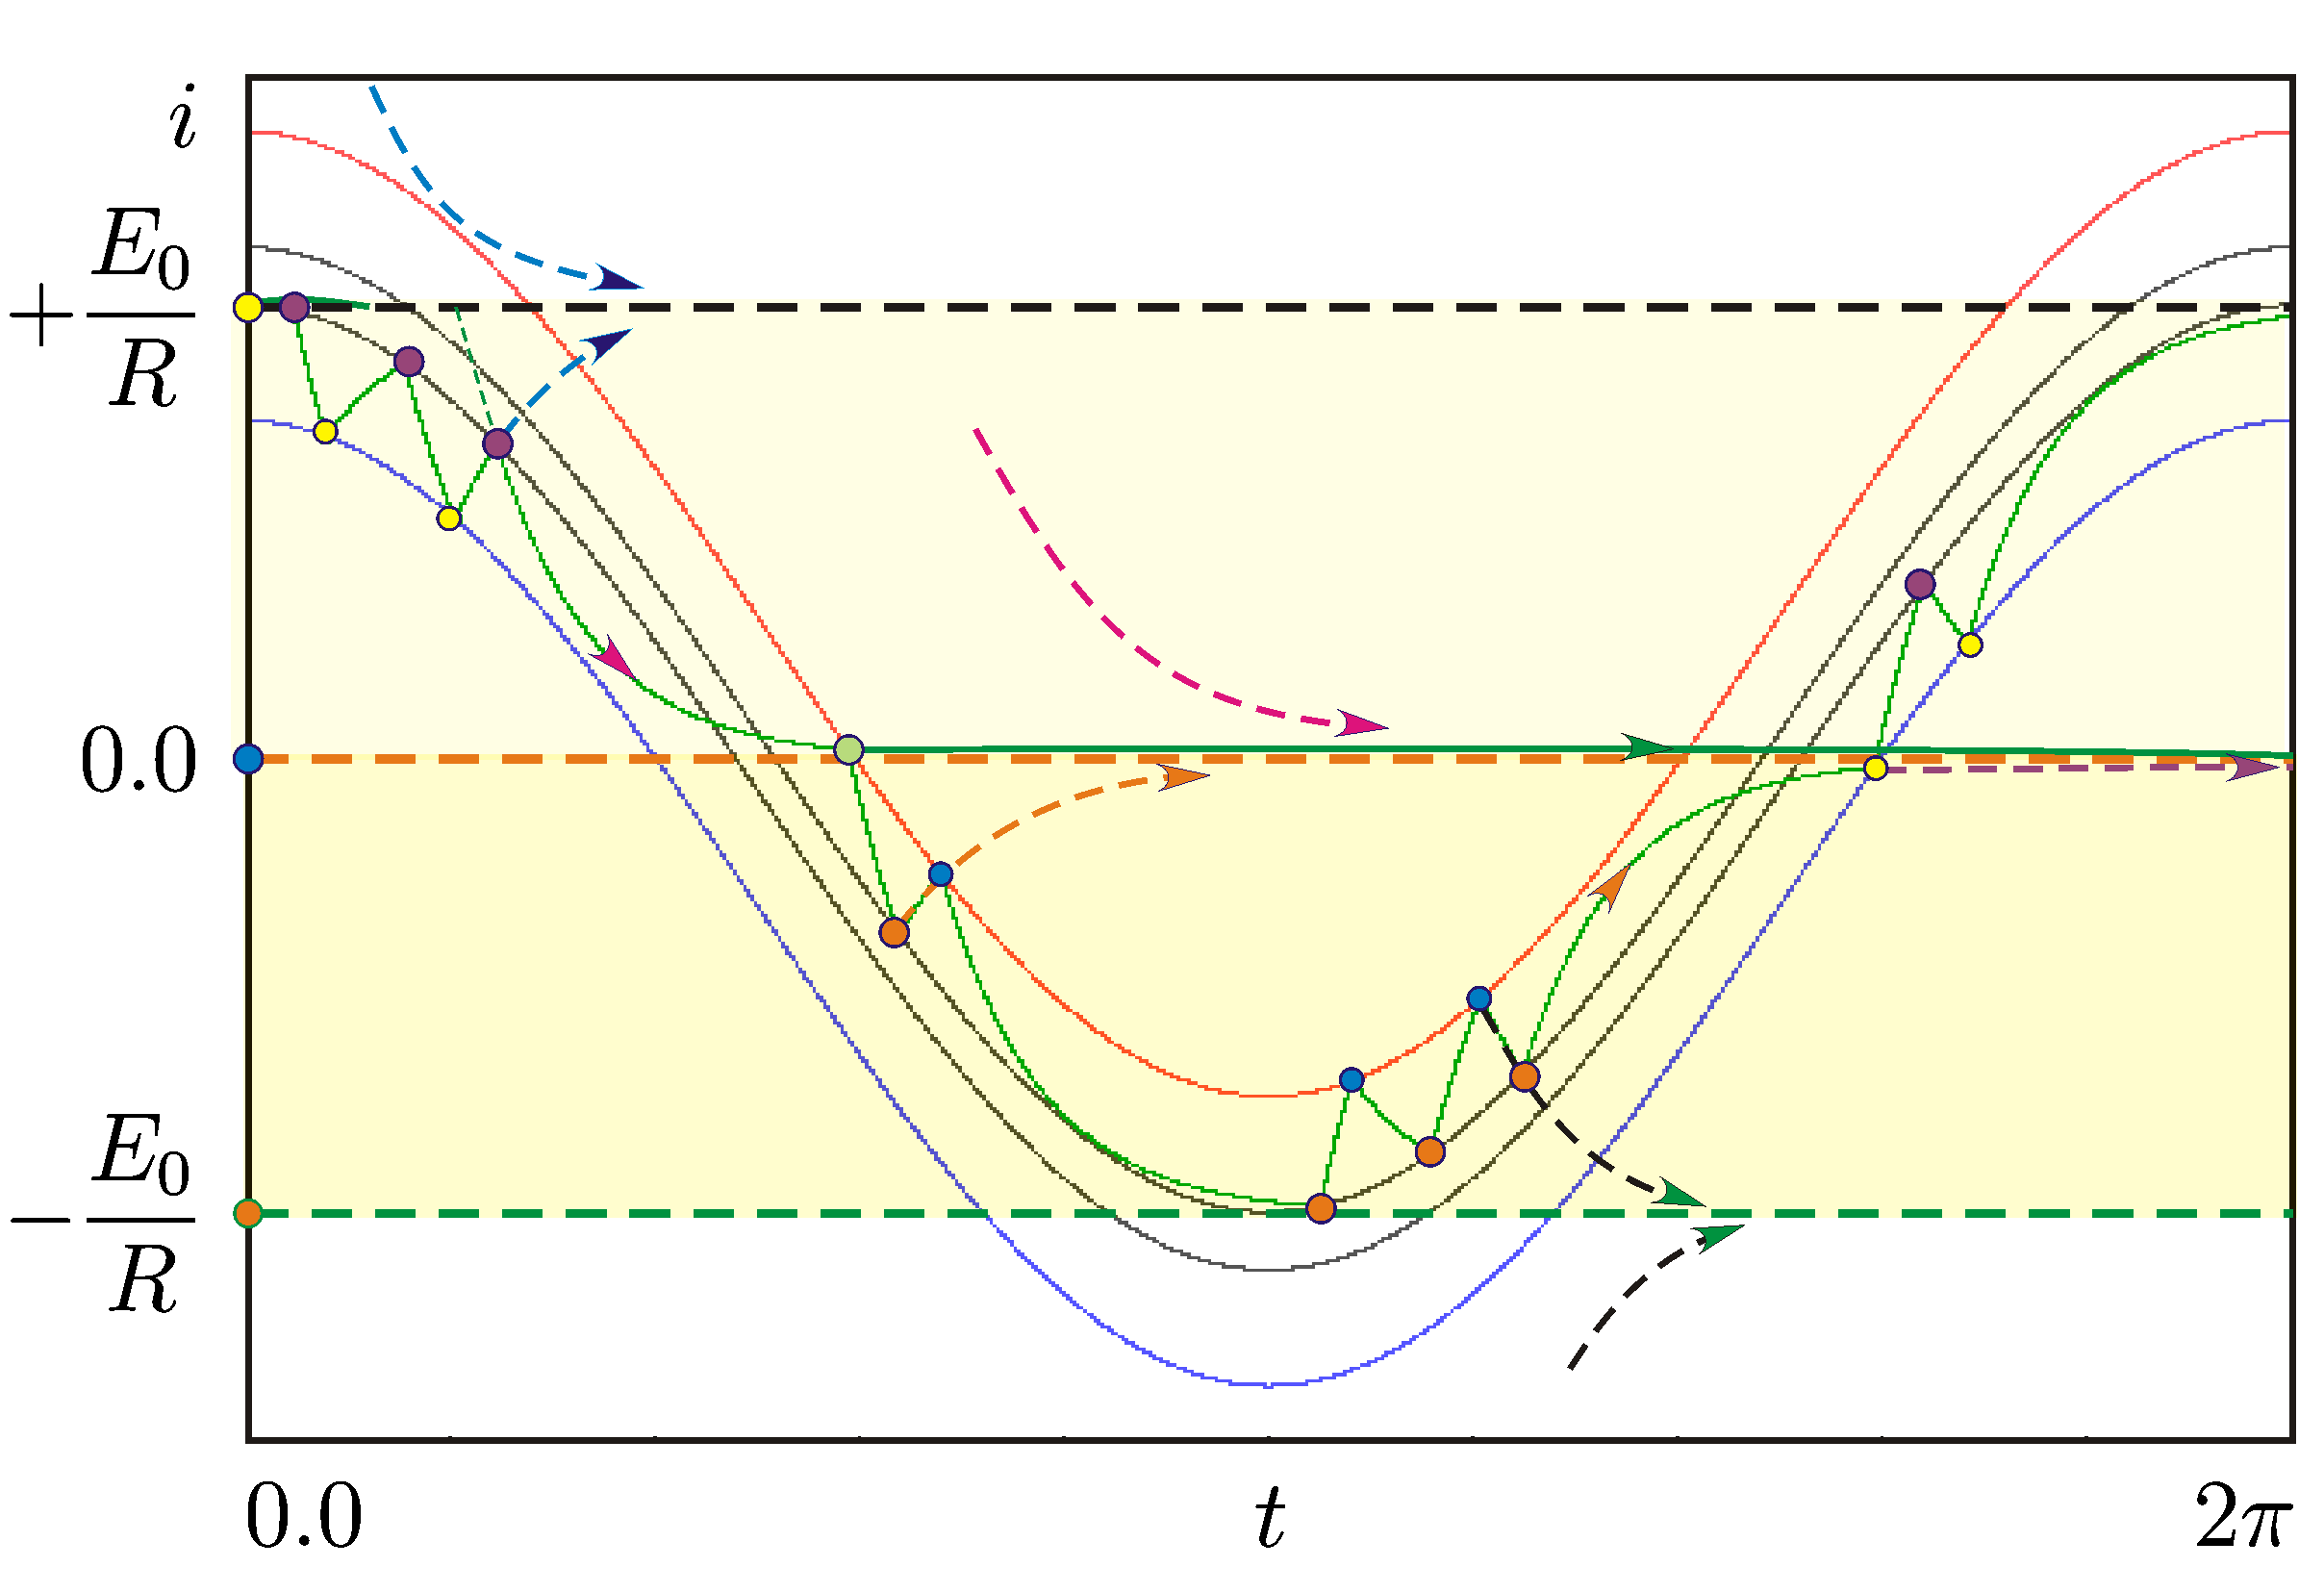
\includegraphics[width=0.8 \textwidth]{Figs/continuous_model.png}
			\end{figure}

			\flushright{[Zhusubaliyev]}
		\end{column}
	\end{columns}
\end{frame}

\begin{frame}{Discrete Model}
	\only<1>{
		\vspace{-2em}
		\begin{align*}
			\theta_{n+1} & =  F(\theta_n) \mod 2 \pi
			\\
			F(\theta)    & = \begin{cases}
				                 F_1(\theta) & \text{if } q \cdot \cos(\theta) > 0 \\
				                 F_2(\theta) & \text{if } q \cdot \cos(\theta) < 0
			                 \end{cases}
			\\
			F_1(\theta)  & = \begin{cases}
				                 \theta + z^{+} + z_{1}^{+}     & \text{if } z^{+} < z_{0}^{+} \\
				                 \theta + z_{0}^{+} + z_{2}^{+} & \text{if } z^{+} > z_{0}^{+}
			                 \end{cases}
			\\
			F_2(\theta)  & = \begin{cases}
				                 \theta + z^{-} + z_{1}^{-}     & \text{if } z^{-} < z_{0}^{-} \\
				                 \theta + z_{0}^{-} + z_{2}^{-} & \text{if } z^{-} > z_{0}^{-}
			                 \end{cases}
		\end{align*}

		\vspace{1em}
		Values of $ z^{+}, z_{1}^{+}, z_{0}^{+}, z_{2}^{+}, z^{-}, z_{1}^{-}, z_{0}^{-}, \text{ and } z_{2}^{-}$?
	}
	\only<2>{
		\vspace{-3em}
		\begin{align*}
			(q \cdot \cos(\theta) - \chi_{c}) \cdot e^{\lambda \cdot z^{+}}
			 & = q \cdot \cos(\theta + z^{+}) - \chi_{0}                  \\
			(q \cdot \cos(\theta + z^{+}) - \chi_{0} - 1) \cdot e^{\lambda \cdot z_{1}^{+}} + 1
			 & = q \cdot  \cos(\theta + z^{+} + z_{1}^{+}) - \chi_{c}     \\
			(q \cdot \cos(\theta) - \chi_{c}) \cdot e^{\lambda \cdot z_{0}^{+}}
			 & = q \cdot \cos(\theta + z_{0}^{+}) + \chi_{0}              \\
			(q \cdot \cos(\theta + z_{0}^{+} + z_{2}^{+}) + \chi_{0} + 1) \cdot e^{\lambda \cdot z_{2}^{+}} - 1
			 & = q \cdot  \cos(\theta + z_{0}^{+} + z_{2}^{+}) + \chi_{c} \\[1em]
			(q \cdot \cos(\theta) + \chi_{c}) \cdot e^{\lambda \cdot z^{-}}
			 & = q \cdot \cos(\theta + z^{-}) + \chi_{0}                  \\
			(q \cdot \cos(\theta + z^{-}) + \chi_{0} + 1) \cdot e^{\lambda \cdot z_{1}^{-}} - 1
			 & = q \cdot  \cos(\theta + z^{-} + z_{1}^{-}) + \chi_{c}     \\
			(q \cdot \cos(\theta) + \chi_{c}) \cdot e^{\lambda \cdot z_{0}^{-}}
			 & = q \cdot \cos(\theta + z_{0}^{-}) - \chi_{0}              \\
			(q \cdot \cos(\theta + z_{0}^{-} + z_{2}^{-}) - \chi_{0} - 1) \cdot e^{\lambda \cdot z_{2}^{-}} + 1
			 & = q \cdot  \cos(\theta + z_{0}^{-} + z_{2}^{-}) - \chi_{c} \\
		\end{align*}
		\vspace{-3em}
		\begin{flushright}
			Smallest positive solutions
			\hfill
			[Akyuz, Avrutin]
		\end{flushright}
	}
\end{frame}

\begin{frame}{Unusual Bifurcation Structure}
	\only<1>{
		\begin{figure}
			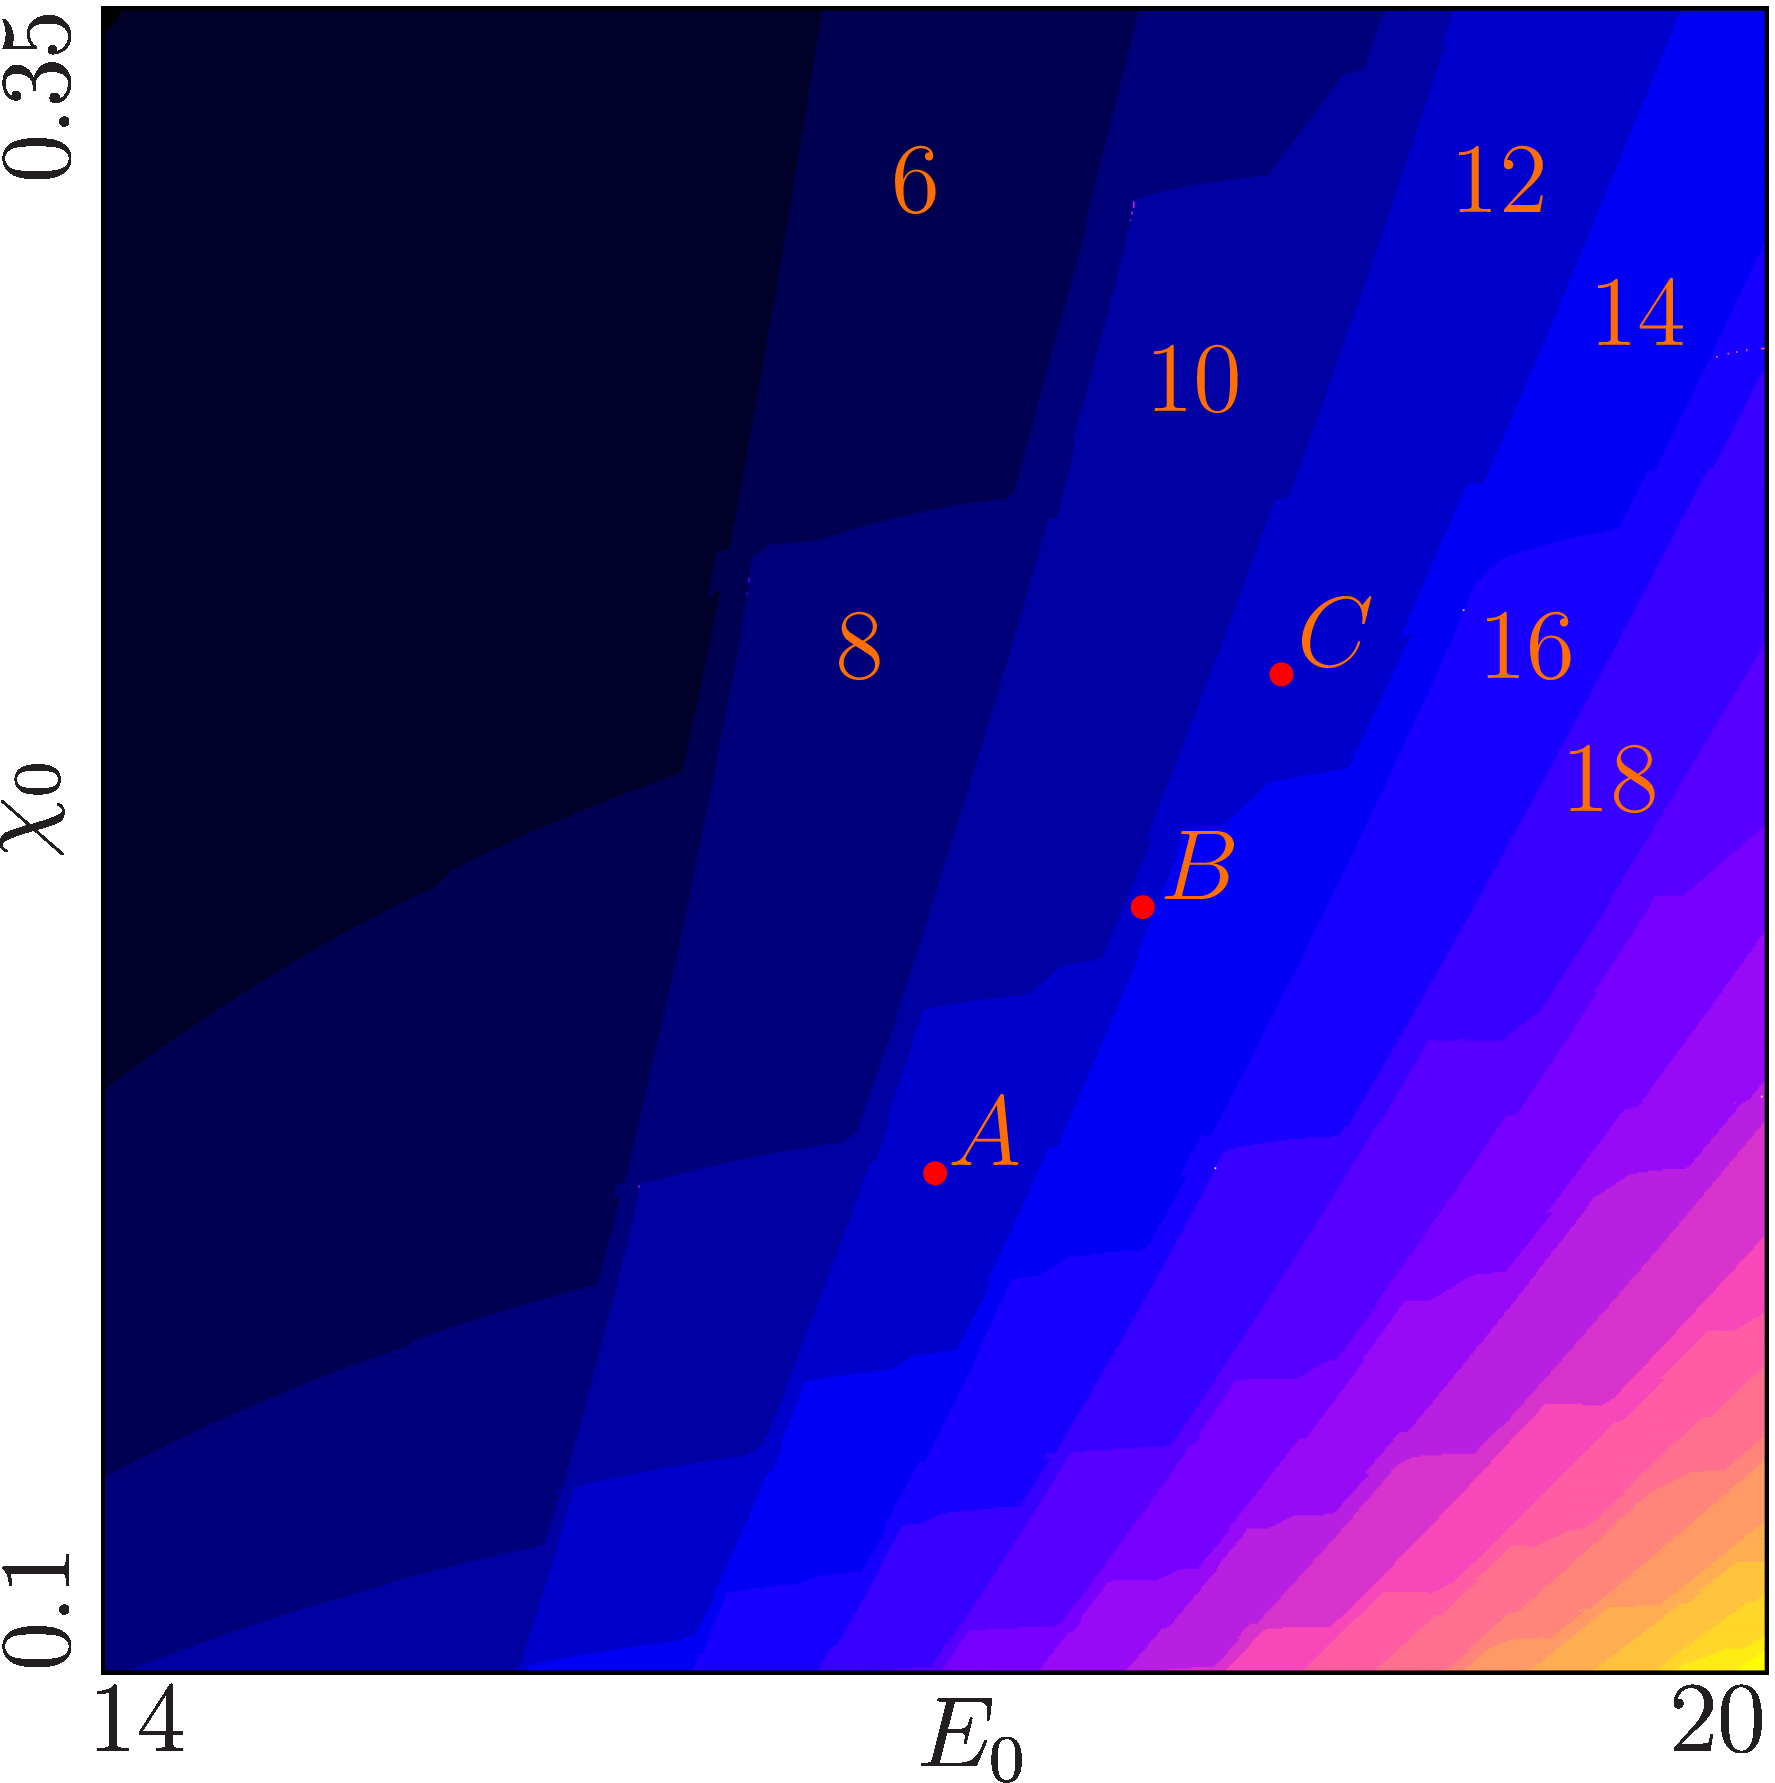
\includegraphics[width=0.45 \textwidth]{Figs/og_model_period.png}
		\end{figure}
	}
	\only<2>{
		\begin{figure}
			\stackunder[5pt]{
				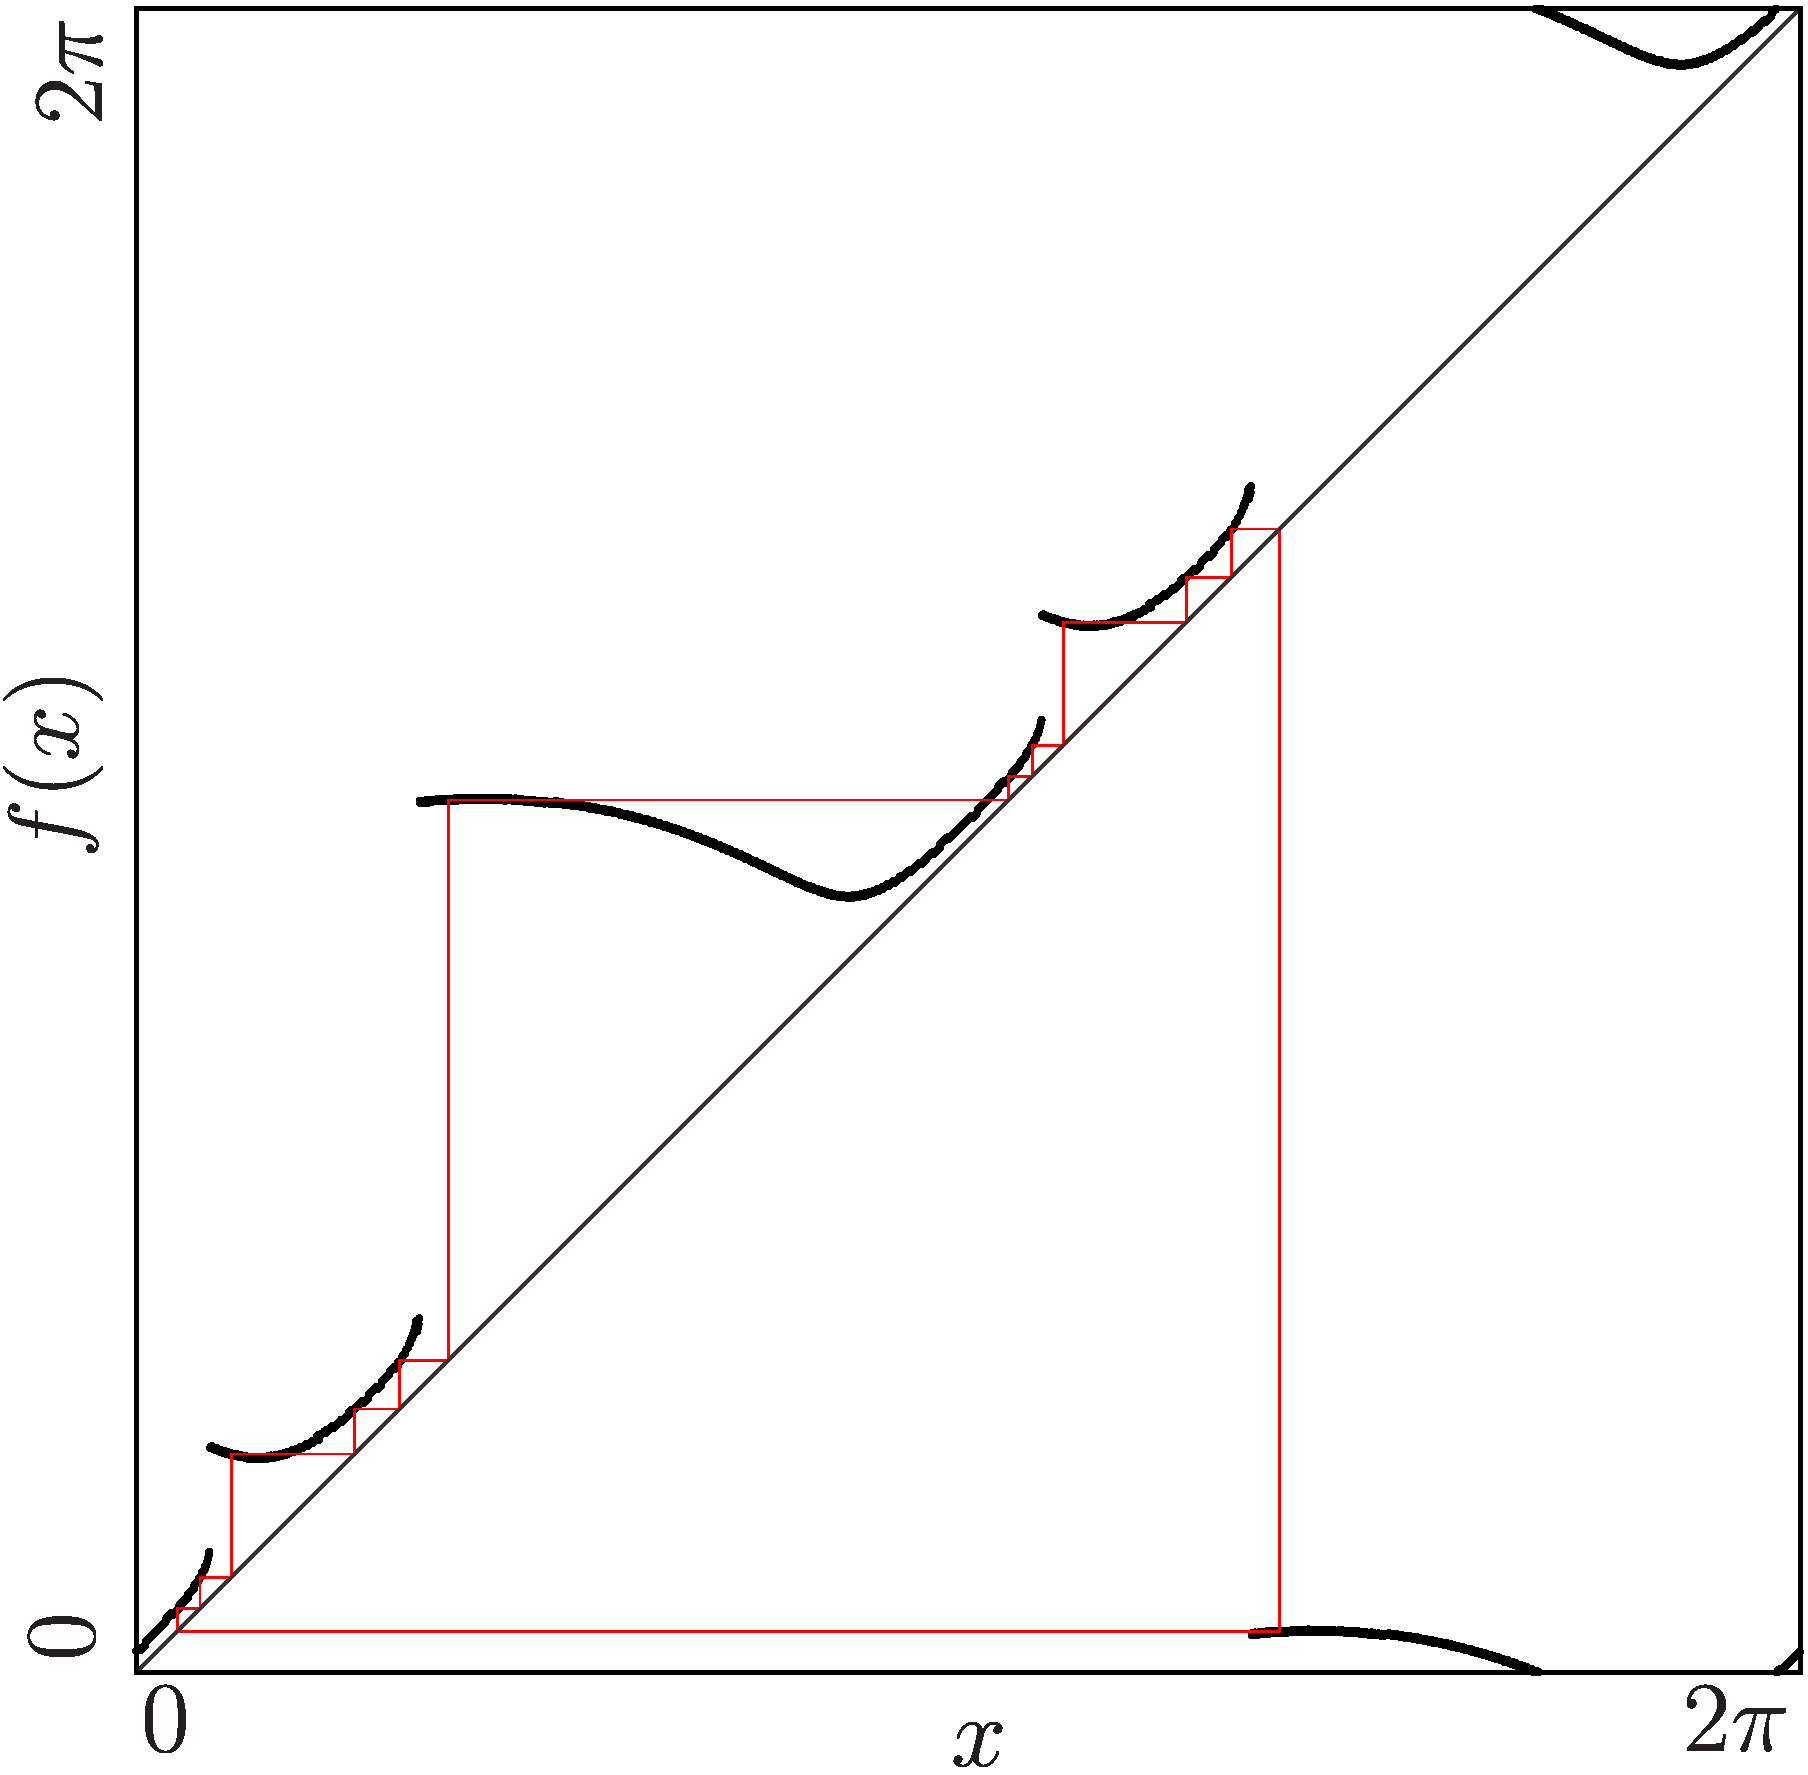
\includegraphics[width=0.3 \textwidth]{Figs/og_model_cycle_a.png}
			}{$\A^3\B^3\C^3\D^3$}
			\stackunder[5pt]{
				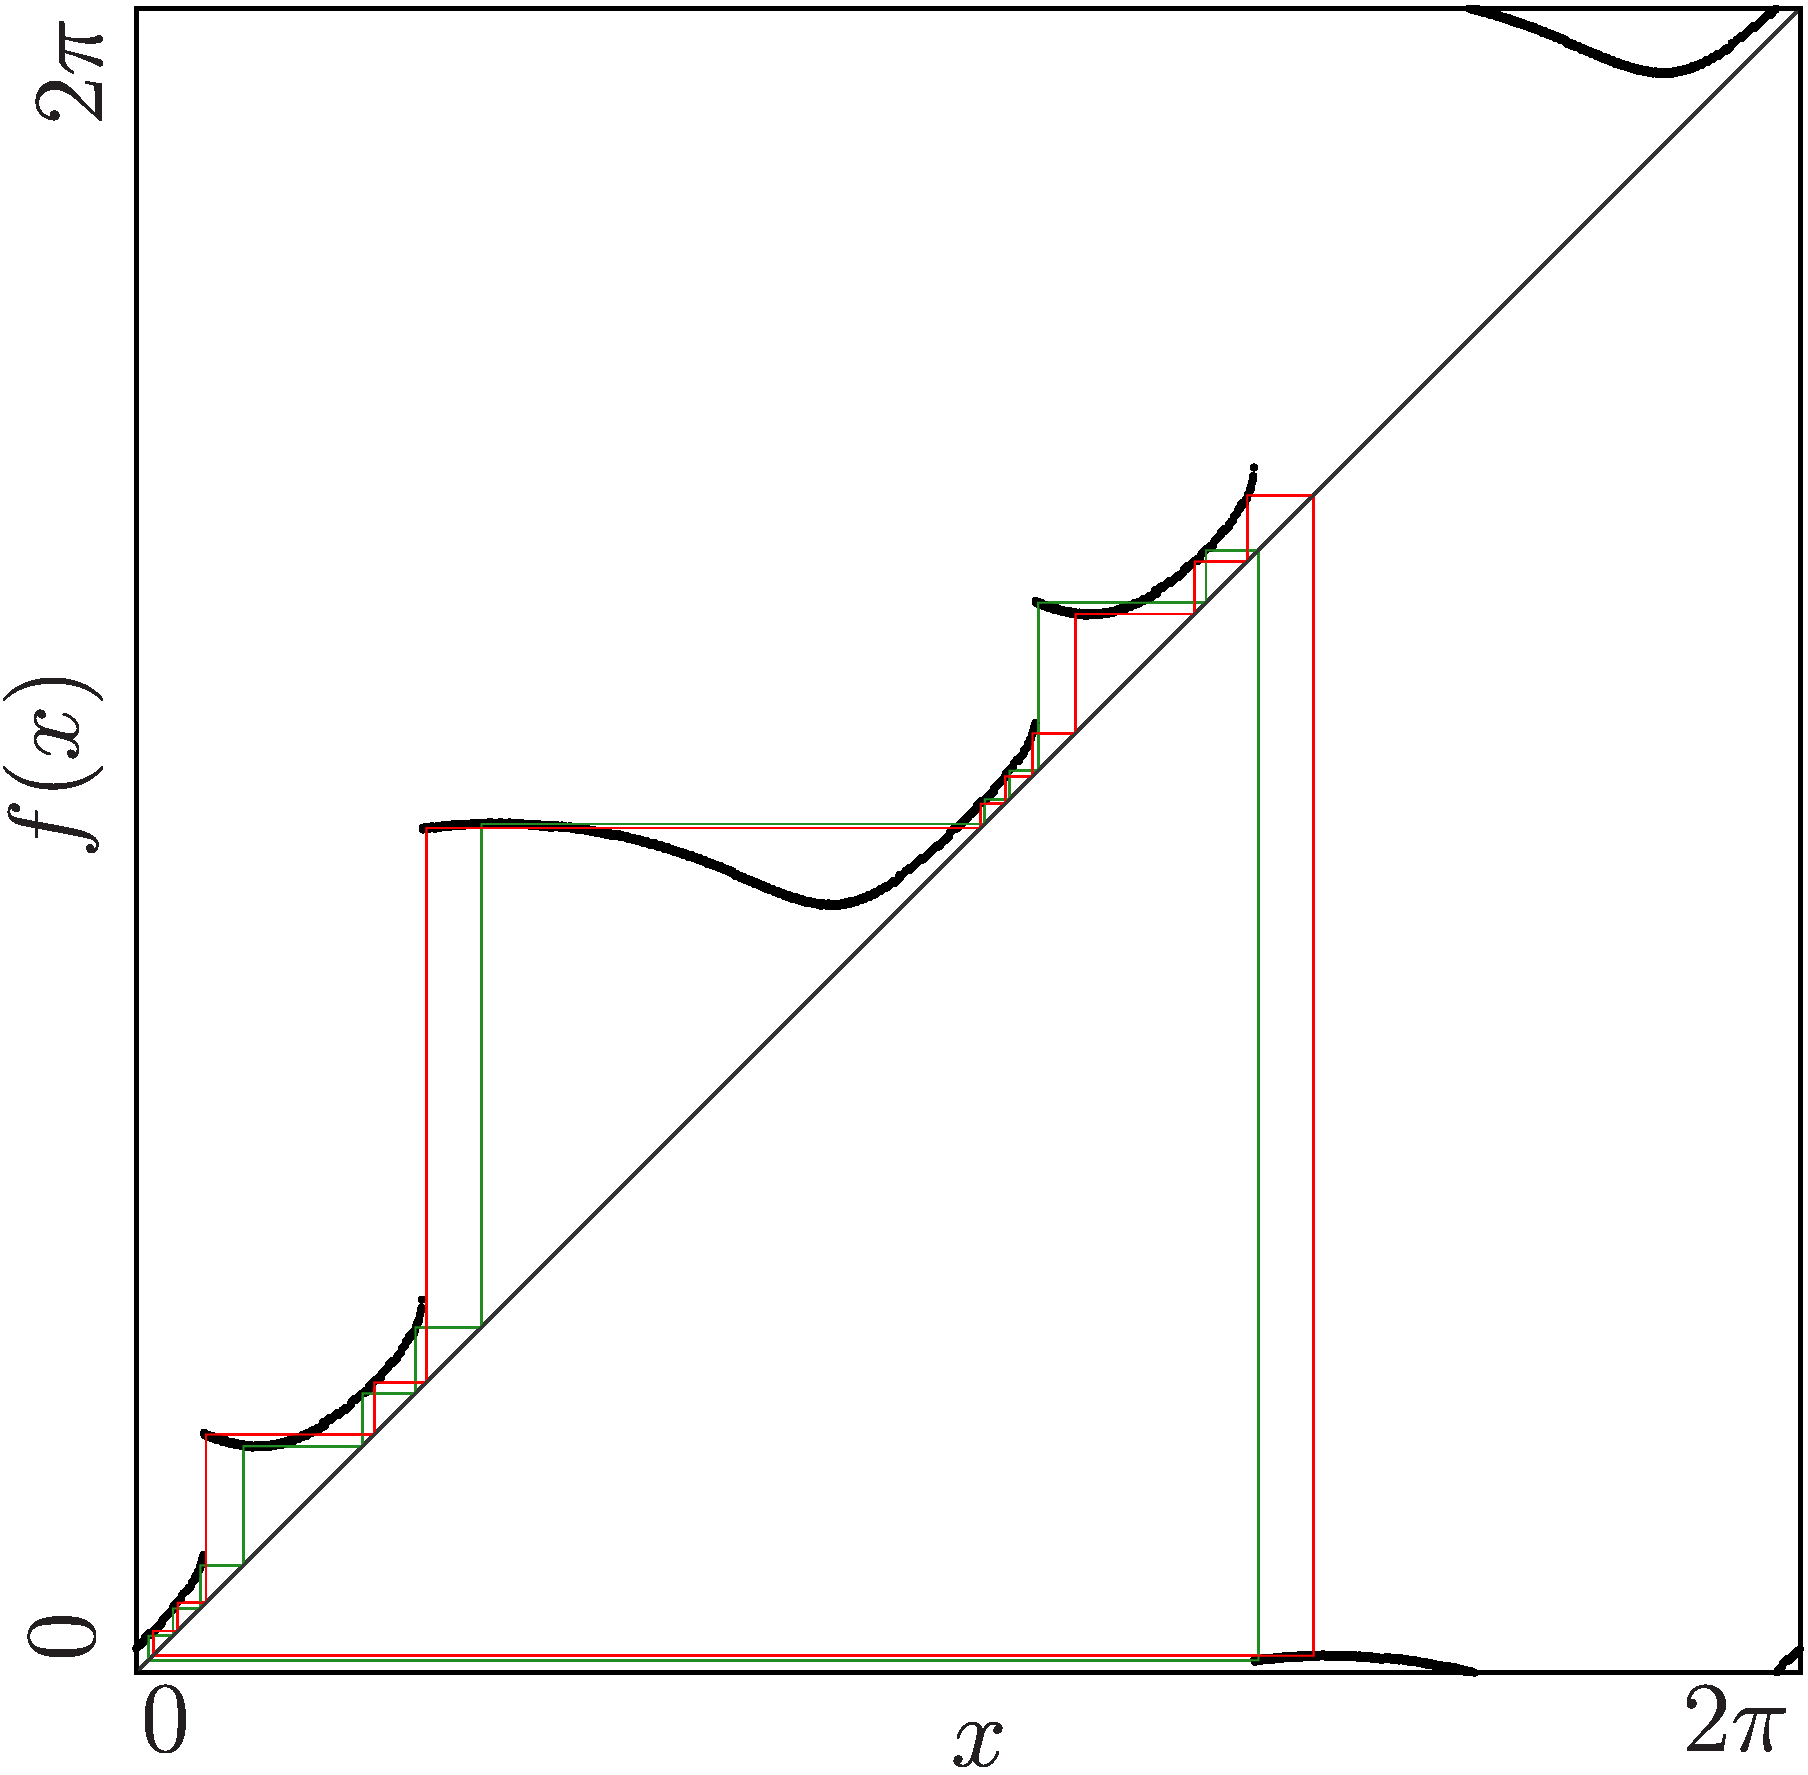
\includegraphics[width=0.3 \textwidth]{Figs/og_model_cycle_b.png}
			}{$\A^3\B^3\C^2\D^4,\:\A^2\B^4\C^3\D^3$}
			\stackunder[5pt]{
				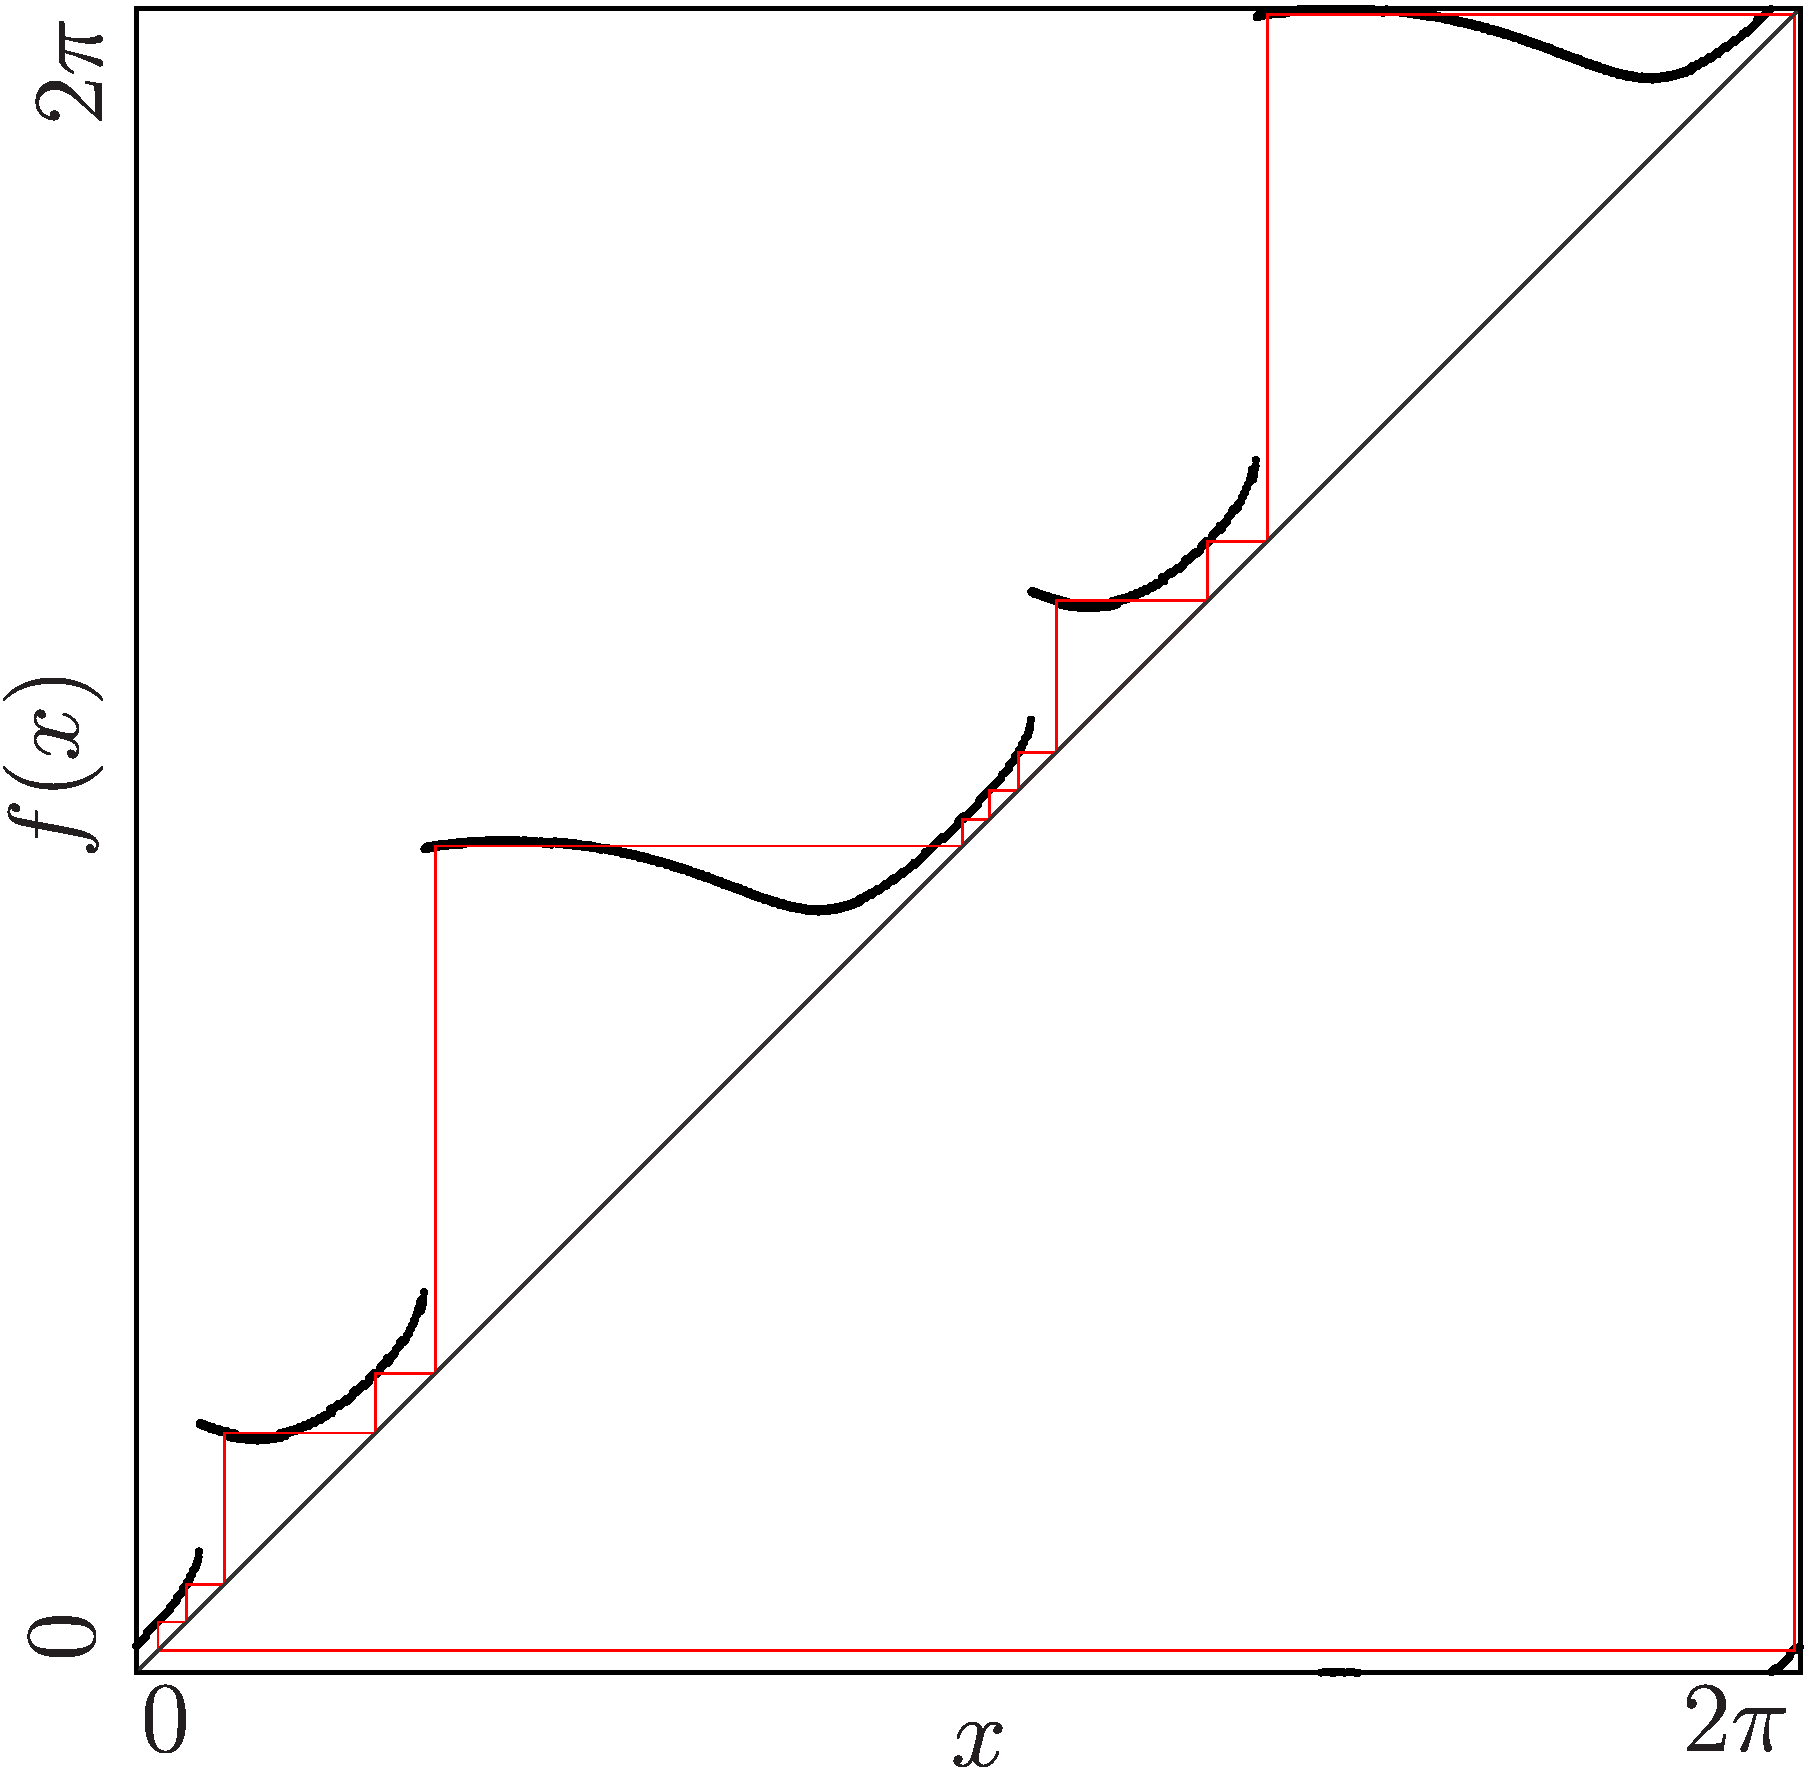
\includegraphics[width=0.3 \textwidth]{Figs/og_model_cycle_c.png}
			}{$\A^2\B^4\C^2\D^4$}
		\end{figure}

		\vspace{1em}
		Symmetry $F(\theta + \pi) = F(\theta) + \pi \mod 2\pi$ \hfill [Akyuz] %\cite{akyuz2022}
	}
\end{frame}

%%% Local Variables:
%%% mode: latex
%%% TeX-master: "../Vortrag_Frauenhofer_Weik"
%%% End:

\sectionframe{Results of my Masters Thesis}
\section{Masters Thesis}

\begin{frame}{Archetypal Model}
	\only<1>{
		\begin{figure}
			\stackunder[5pt]{
				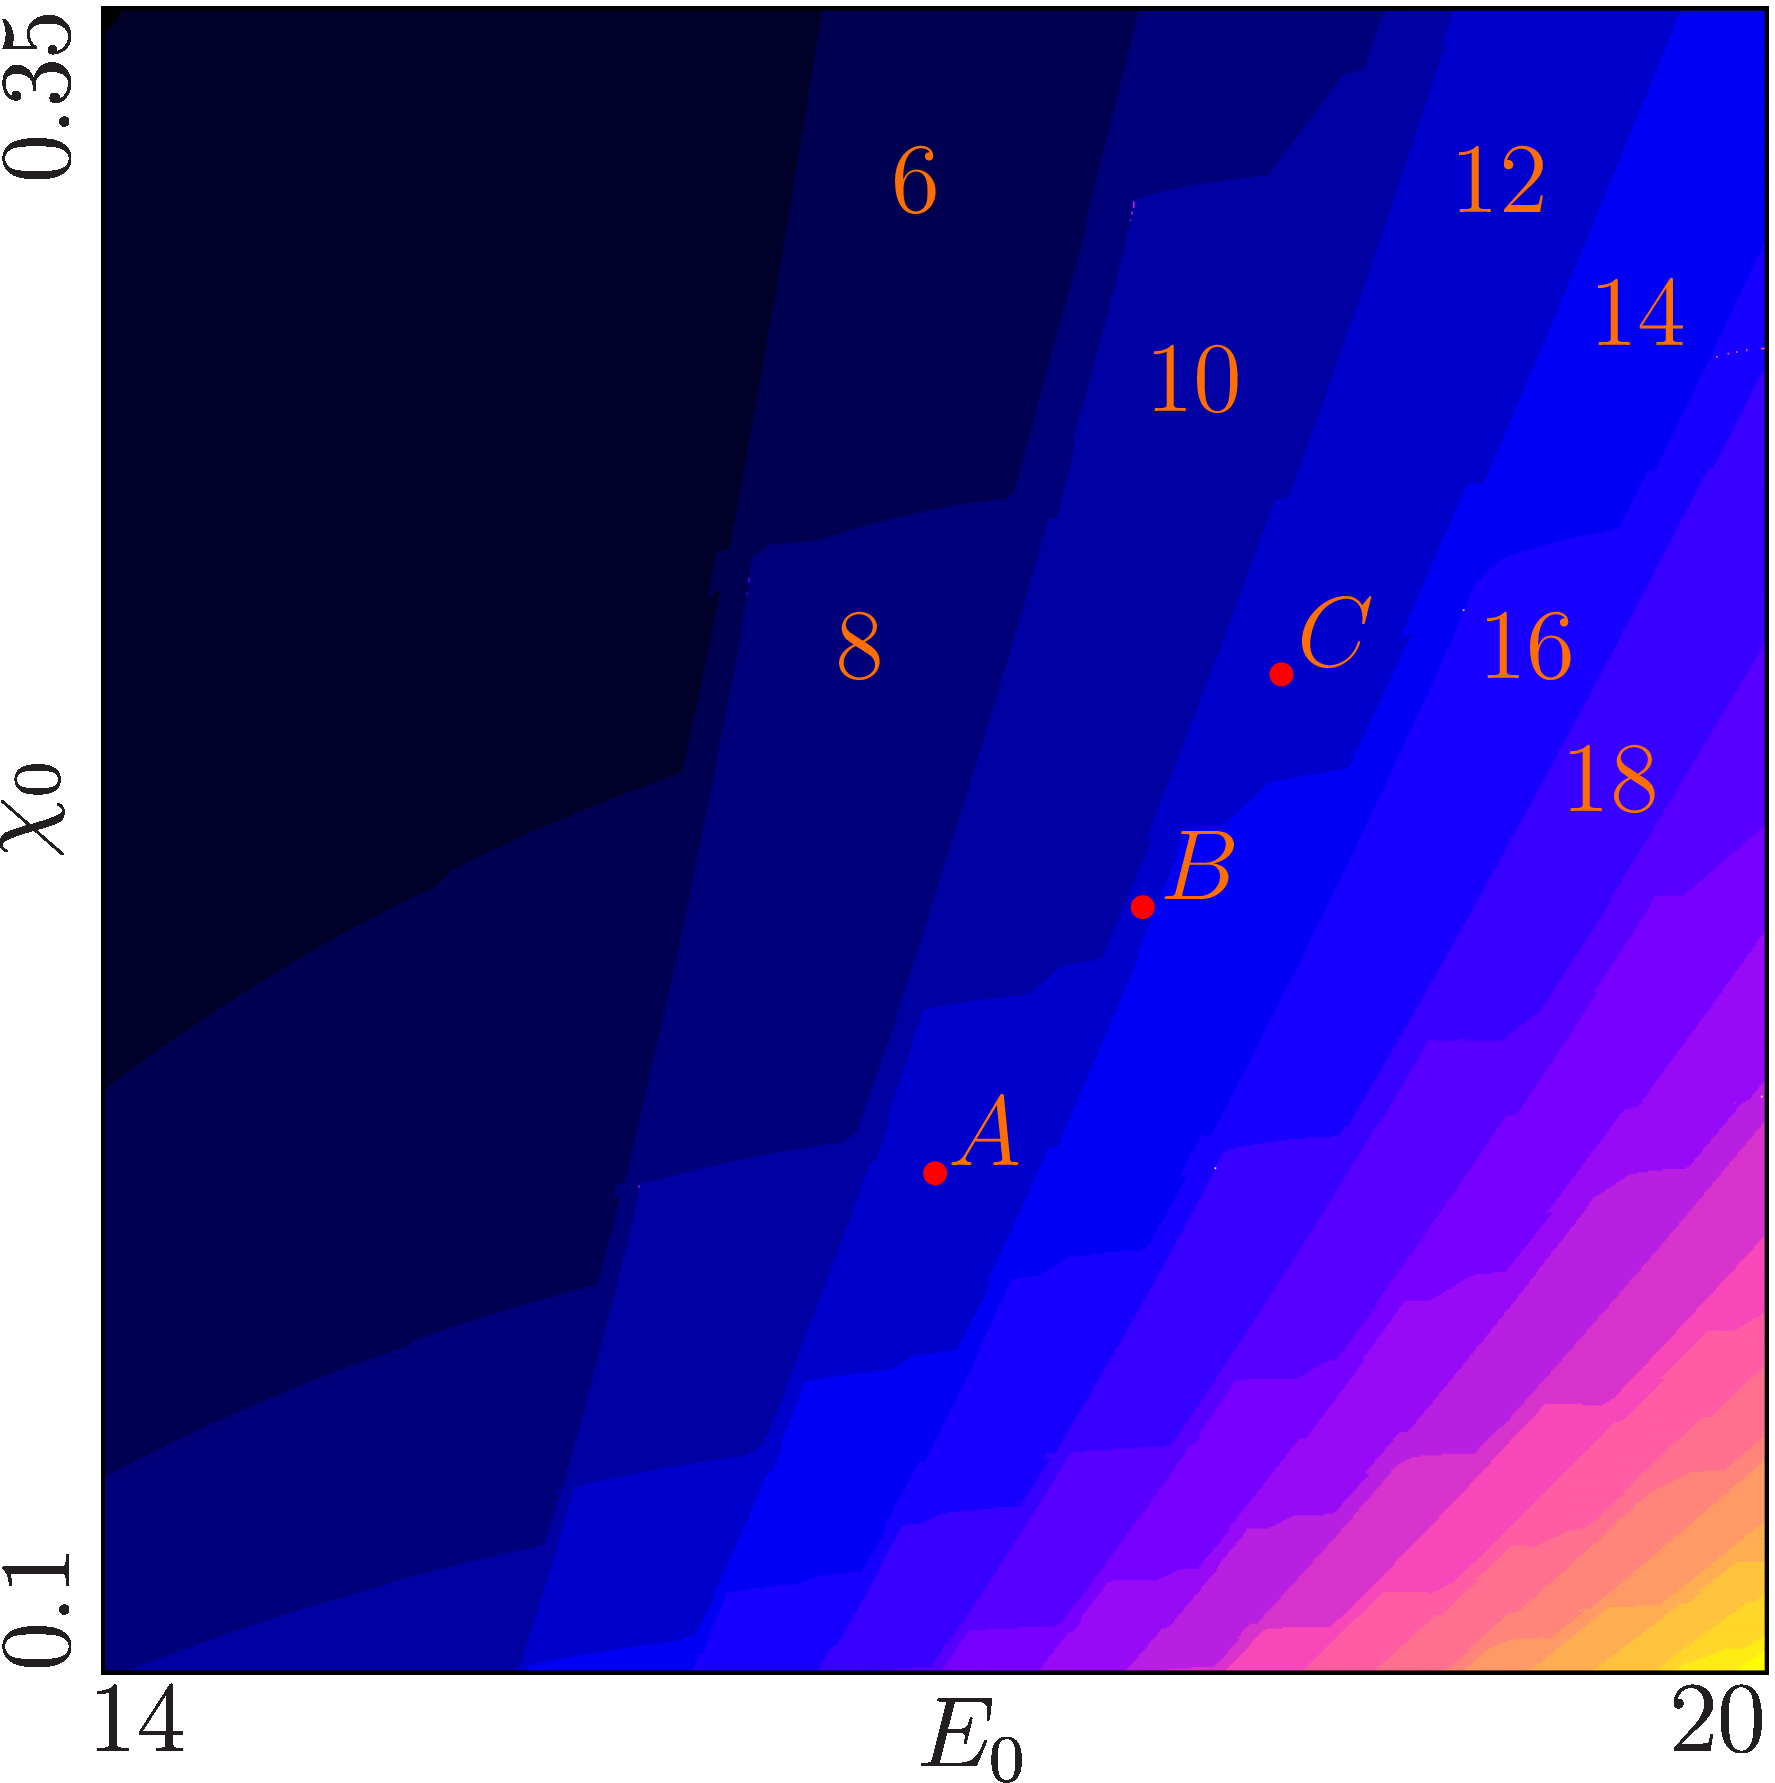
\includegraphics[width=0.4 \textwidth]{Figs/og_model_period.png}
			}{Original model}
			\qquad
			\stackunder[5pt]{
				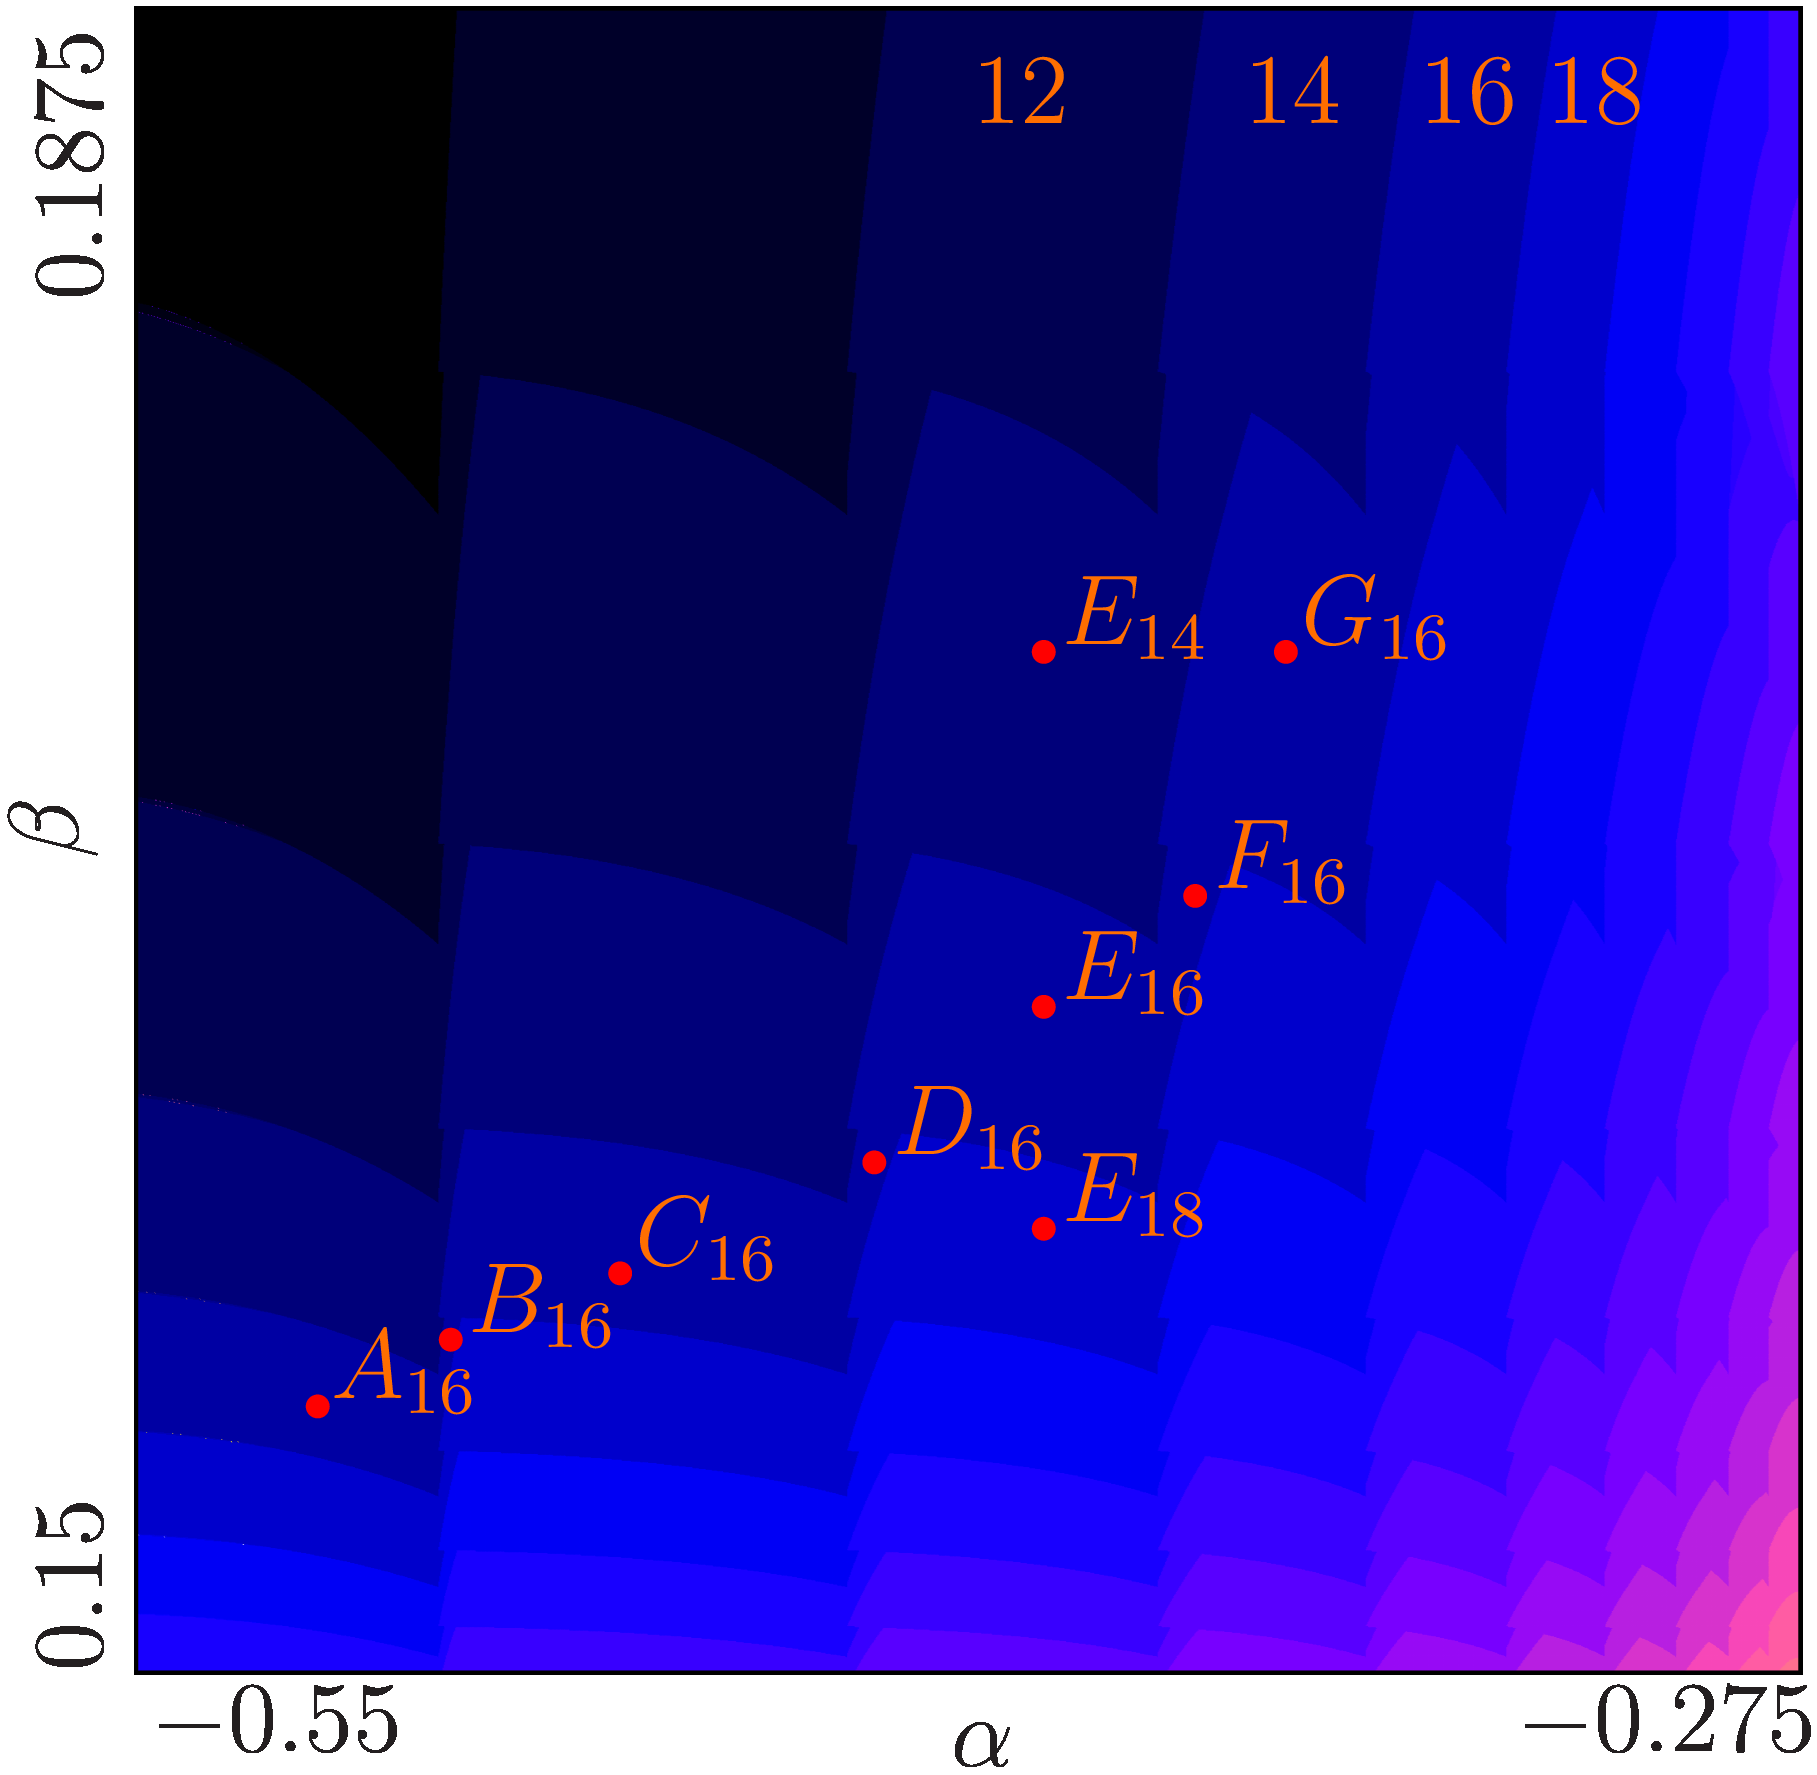
\includegraphics[width=0.41 \textwidth]{Figs/archetypal_model_period.png}
			}{Archetypal model}
		\end{figure}
	}
	\only<2>{
		\begin{figure}
			\centering
			\stackunder[5pt]{
				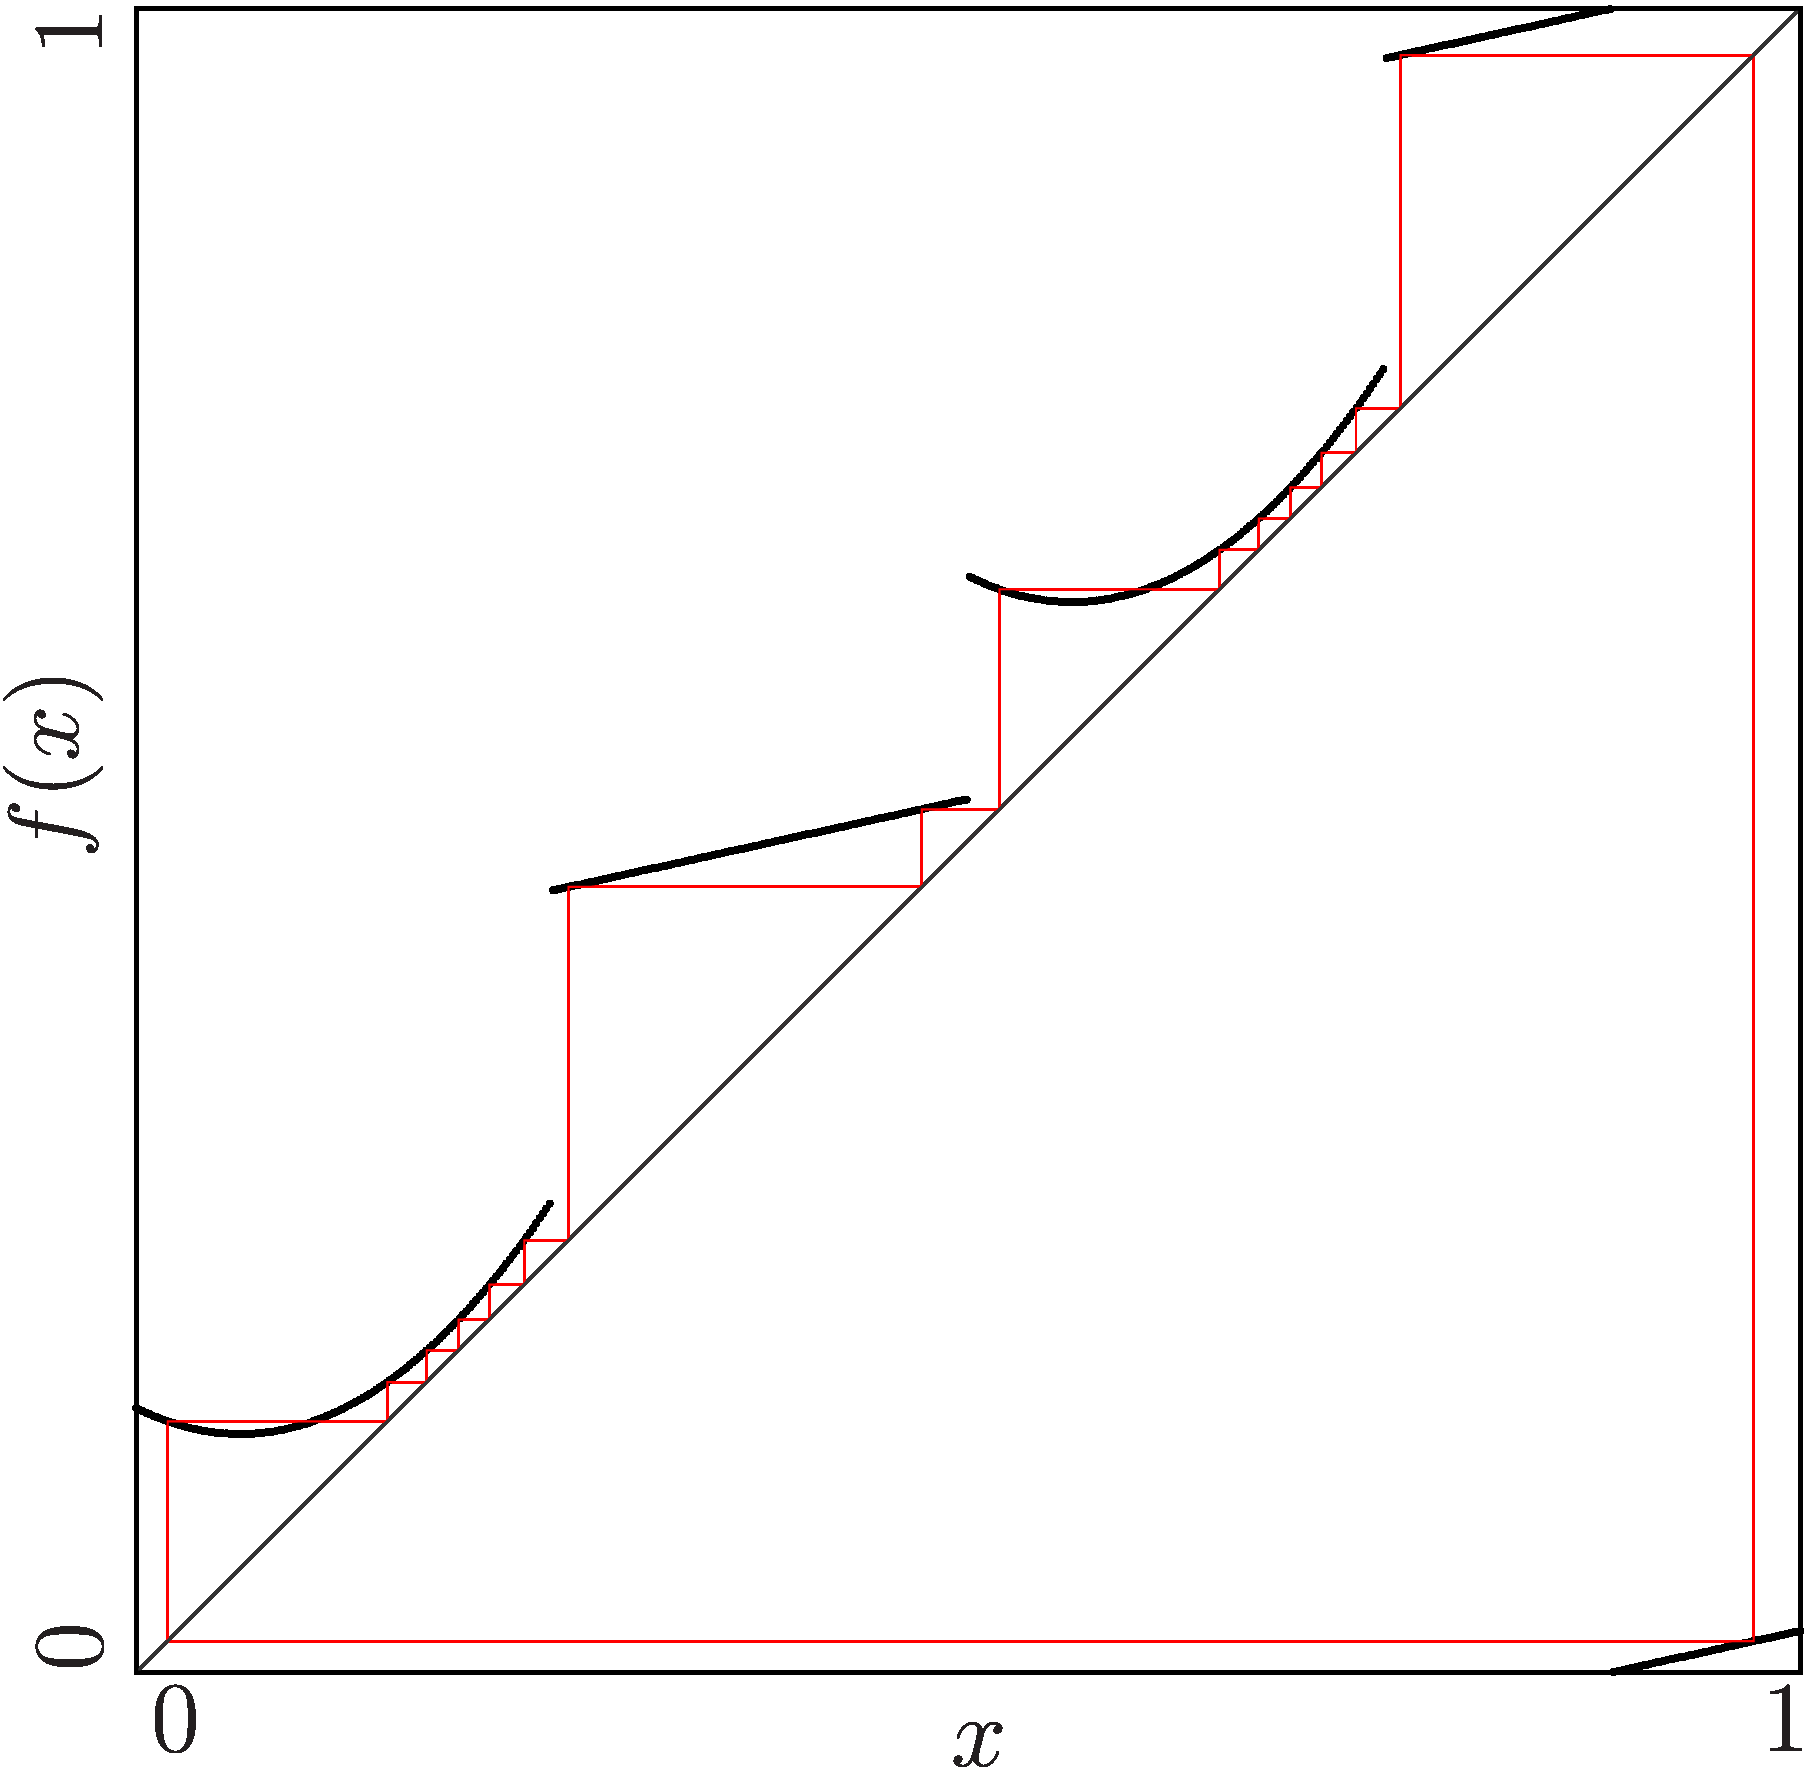
\includegraphics[width=0.3 \textwidth]{Figs/archetypal_model_cycle_c16.png}
			}{$C_{16}:\:\Cycle{\A^6\B^2\C^6\D^2}$}
			\stackunder[5pt]{
				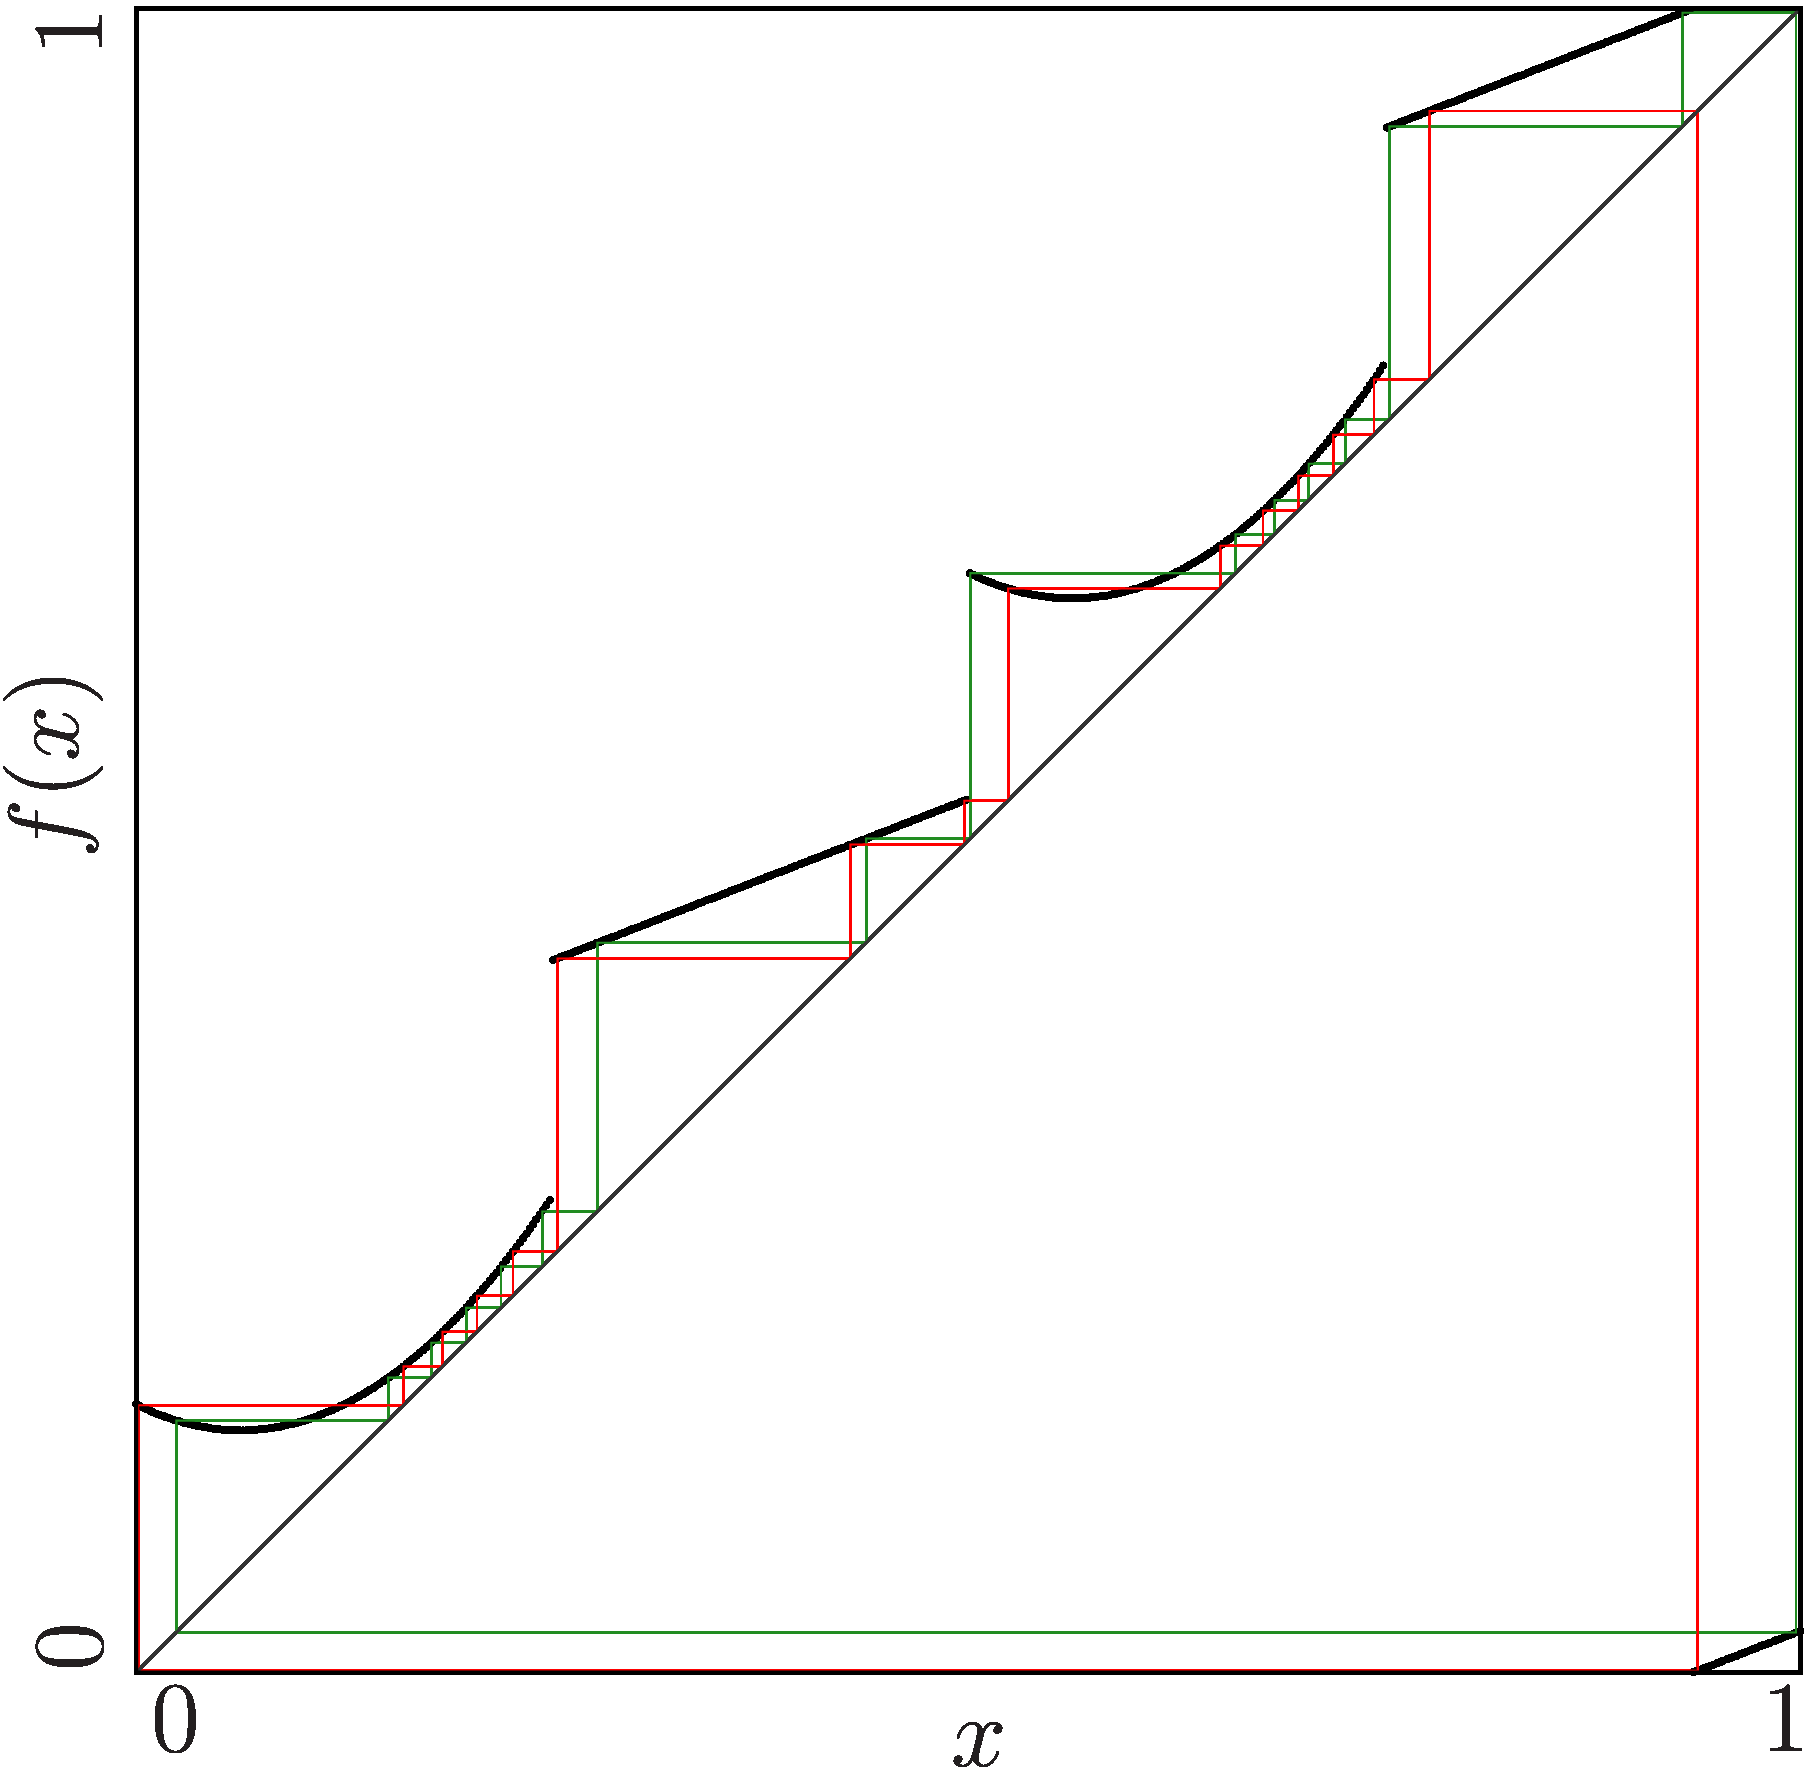
\includegraphics[width=0.3 \textwidth]{Figs/archetypal_model_cycle_d16.png}
			}{$D_{16}:\:\Cycle{\A^6\B^2\C^5\D^3},\Cycle{\A^5\B^3\C^6\D^2}$}
			\stackunder[5pt]{
				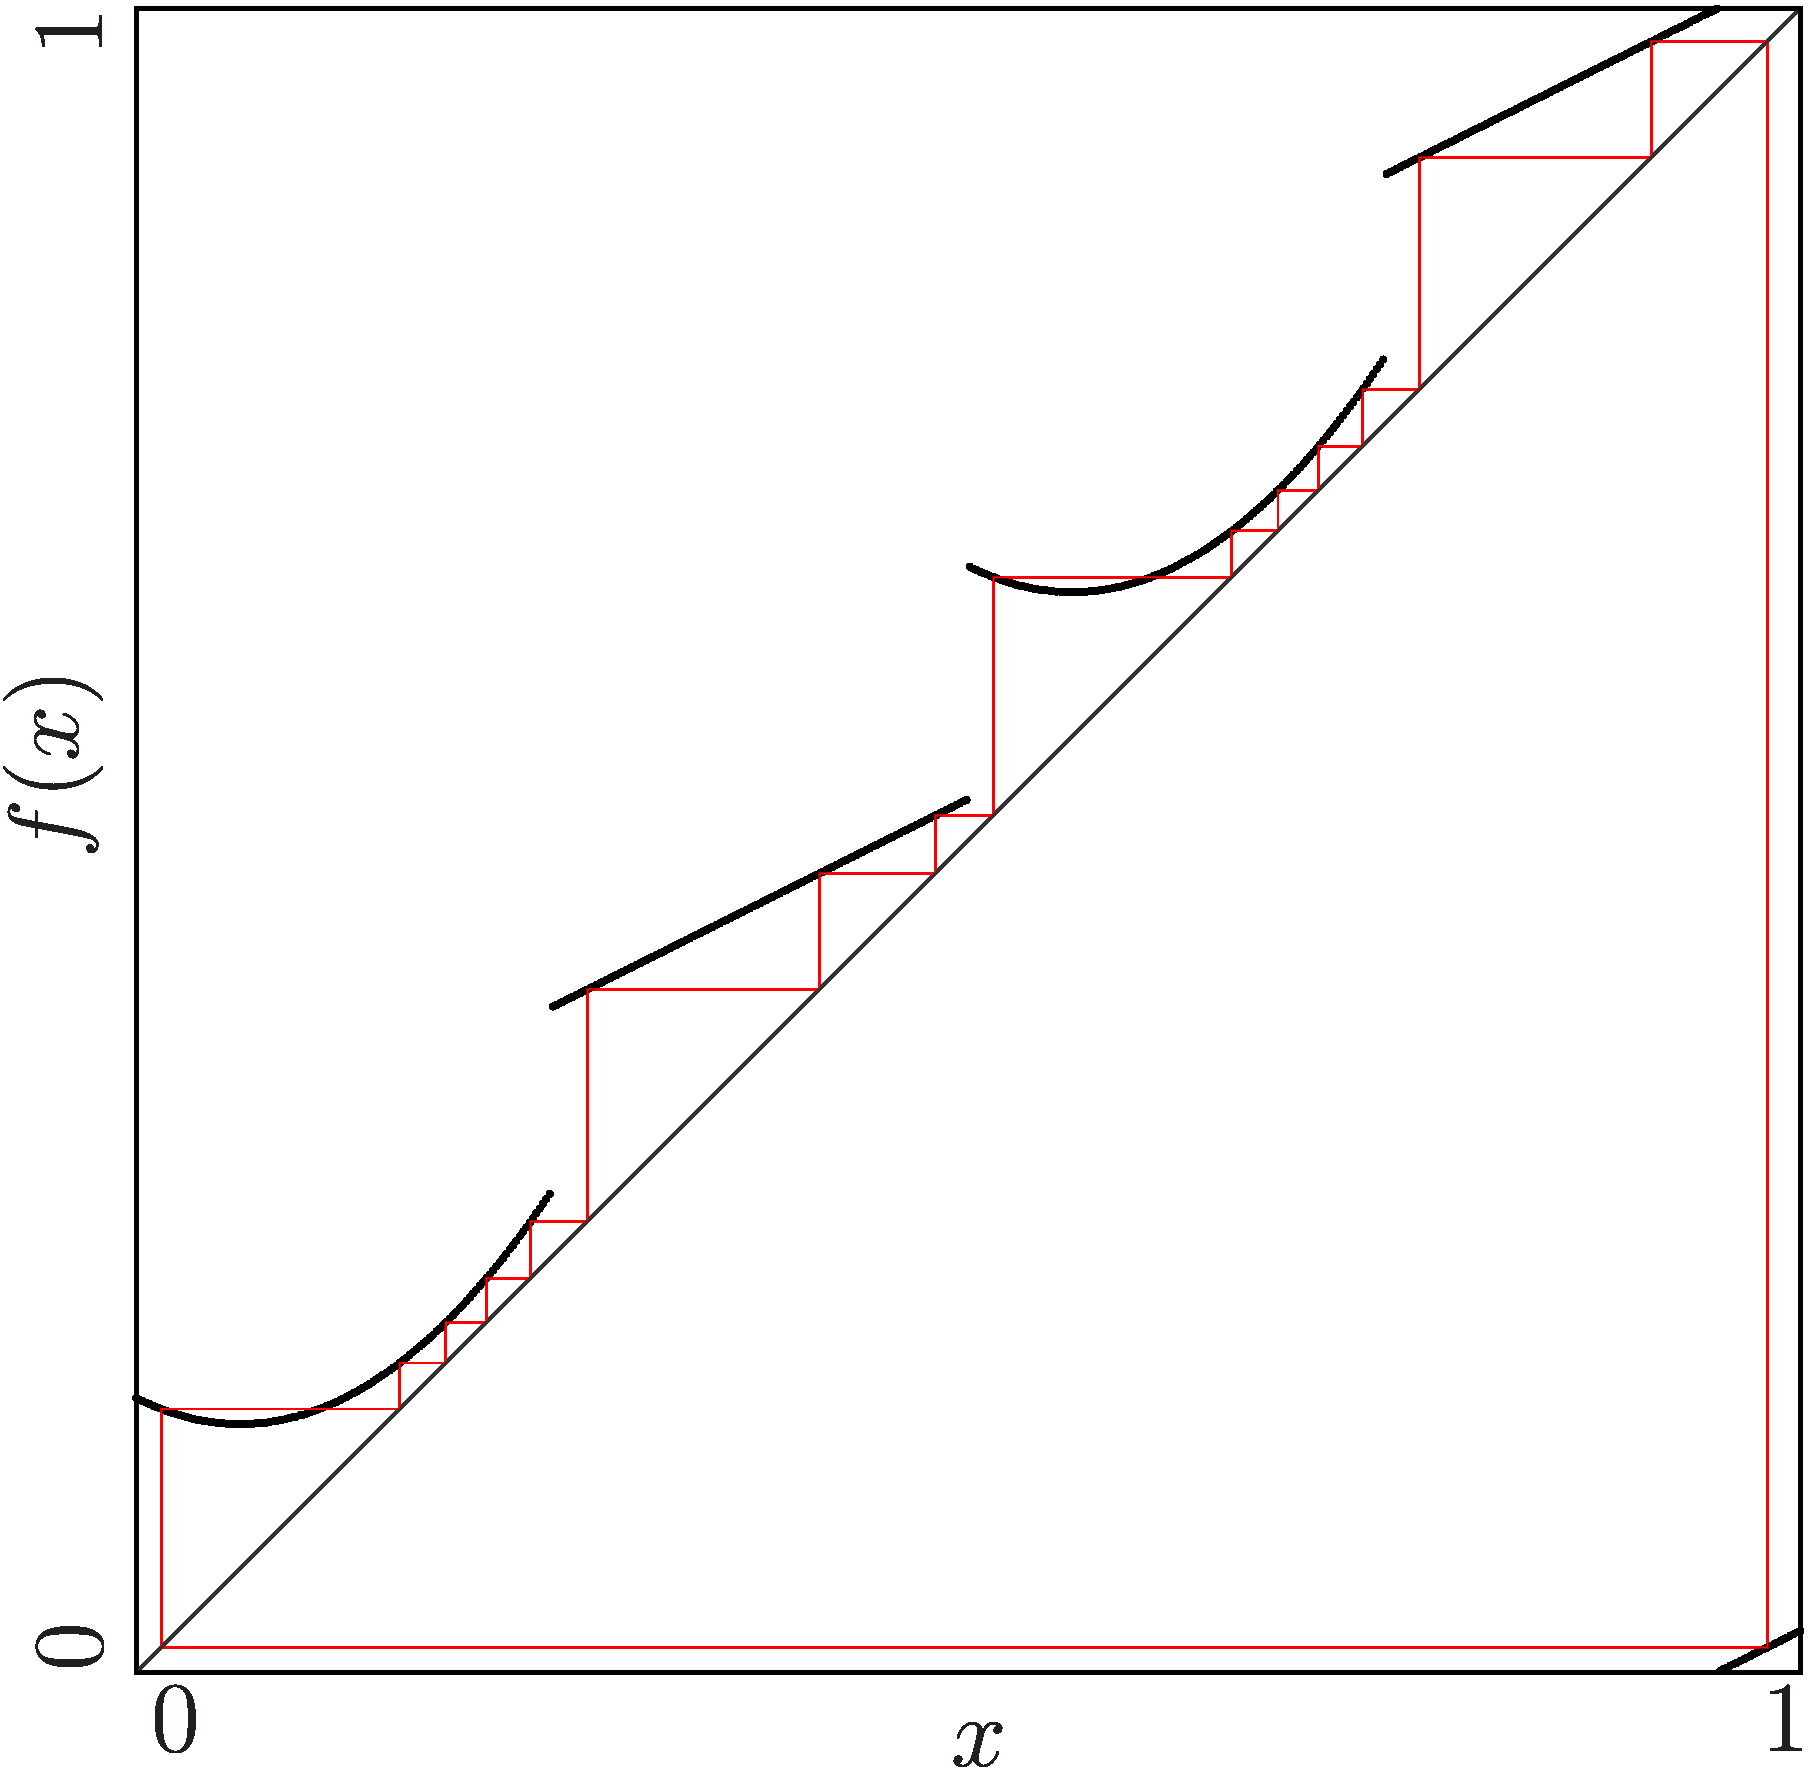
\includegraphics[width=0.3 \textwidth]{Figs/archetypal_model_cycle_e16.png}
			}{$E_{16}:\:\Cycle{\A^5\B^3\C^5\D^3}$}
		\end{figure}
	}
\end{frame}

\begin{frame}{Archetypal Model Equations}
	\vspace{-1.0em}
	\only<1>{
		\begin{align*}
			x_{n+1} = f(x_n) \mod 1
		\end{align*}
		\begin{align*}
			f(x) & = \begin{cases}
				         g(x)                                        & \text{ if } x < \frac{1}{2} \\
				         g\left(x - \frac{1}{2}\right) + \frac{1}{2} & \text{ else}
			         \end{cases}
		\end{align*}
		\begin{align*}
			g(x) & = \begin{cases}
				         g_L(x) = a_L \cdot x^2 + b_L \cdot x + c_L & \text{ if } x < \frac{1}{4} \\
				         g_R(x) = b_R \cdot x + c_R                 & \text{ else}
			         \end{cases}
		\end{align*}
	}
	\only<2>{
		\begin{columns}
			\begin{column}{.7 \textwidth}
				Fixed parameters:
				\begin{align*}
					a_L = 4 \text{ and } b_L = -\tfrac{1}{2}
				\end{align*}
				Variable parameters
				\begin{align*}
					 & c_L, b_R, c_R                                                                                                              \\
					\text{where} \qquad
					 & c_L = \beta,                                                                                                               \\
					 & b_R = -4 \cdot g_R\left(\tfrac{1}{4}\right) + 4 \cdot g_R\left(\tfrac{1}{2}\right),                                        \\
					 & c_R = 2 \cdot g_R\left(\tfrac{1}{4}\right) - 1 \cdot g_R\left(\tfrac{1}{2}\right),                                         \\[1em]
					\text{and} \qquad
					 & g_R\left(\tfrac{1}{4}\right) = \alpha, \text{and } g_R\left(\tfrac{1}{2}\right) = \tfrac{1}{2} + \epsilon \text{ is fixed}
				\end{align*}
			\end{column}
			\begin{column}{.3 \textwidth}
				\begin{figure}
					\centering
					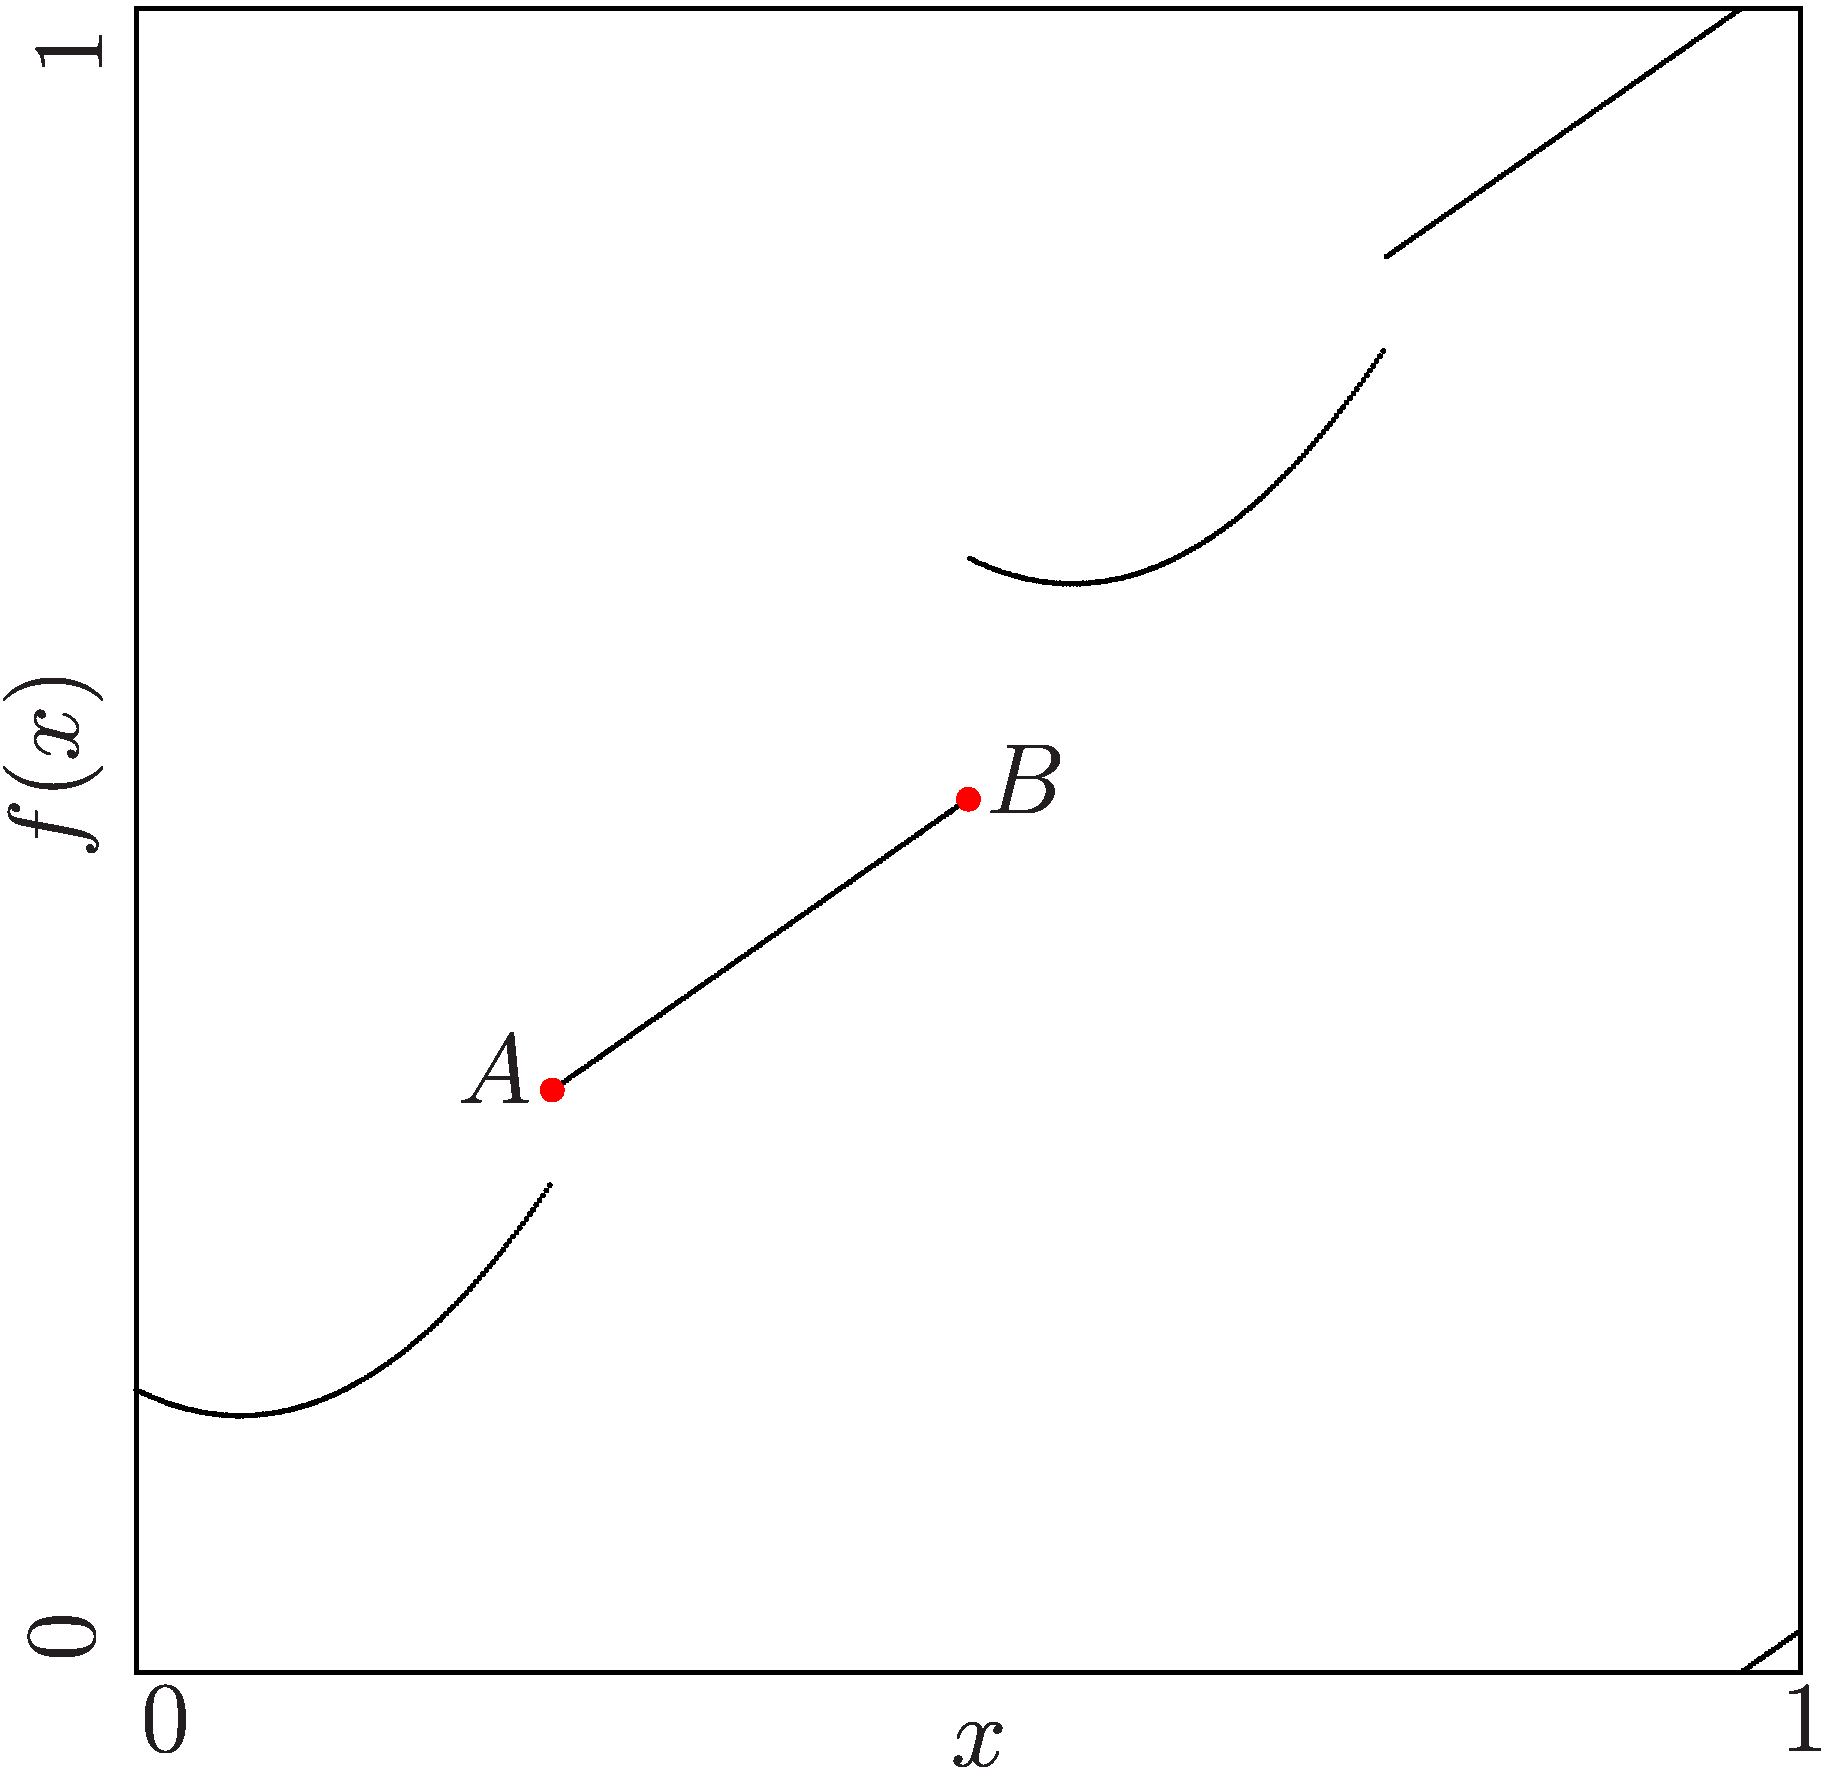
\includegraphics[height=.5 \textheight]{Figs/archetypal_model_parameter_effects_illustration.png}
				\end{figure}
			\end{column}
		\end{columns}
	}
\end{frame}

\begin{frame}{Archetypal Model Results}
	\begin{itemize}
		\item Description of the bifucation structure
		\item Explanation of coexisting cycles via the symmetry
		\item Explanation of double border collisions via the symmetry
		\item Discovery of 4 coexisting cycles not discovered in the original model
		      \begin{itemize}
			      \item Confirmation of 4 coexisting cycles in the original model
		      \end{itemize}
	\end{itemize}
\end{frame}

\begin{frame}{Period-Adding?}
	\vspace{-1em}
	\begin{itemize}
		\item Chains overlap
		\item What happens, when they no longer overlap?
		      \vspace{1em}
		\item Prediction: Period-Adding
		      %\item Turns up often
		      %\item E.g. Edge of main bubble of mandelbrot set
	\end{itemize}
	\begin{figure}
		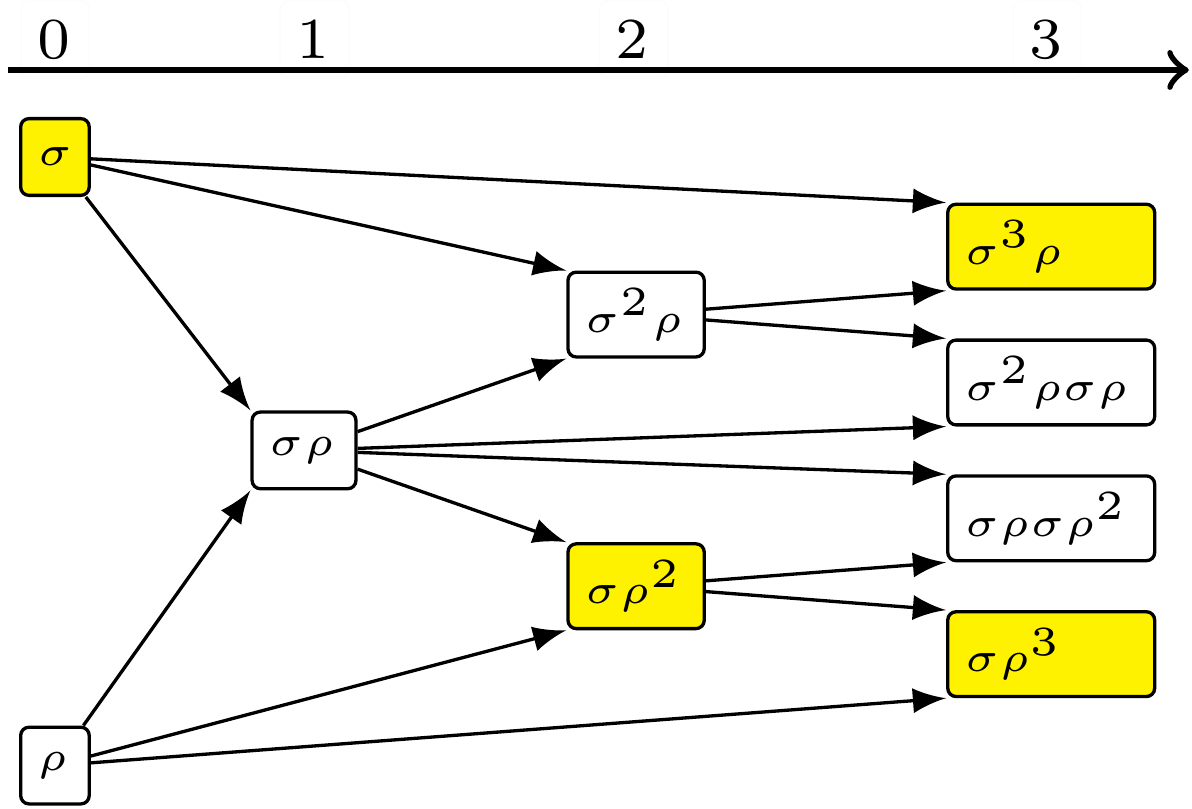
\includegraphics[height=.5 \textheight]{Figs/Trees/ClassicalAdding/adding.png}
	\end{figure}
\end{frame}

\begin{frame}{Archetypal Model with Different Parameters}
	\only<1>{
		\begin{figure}
			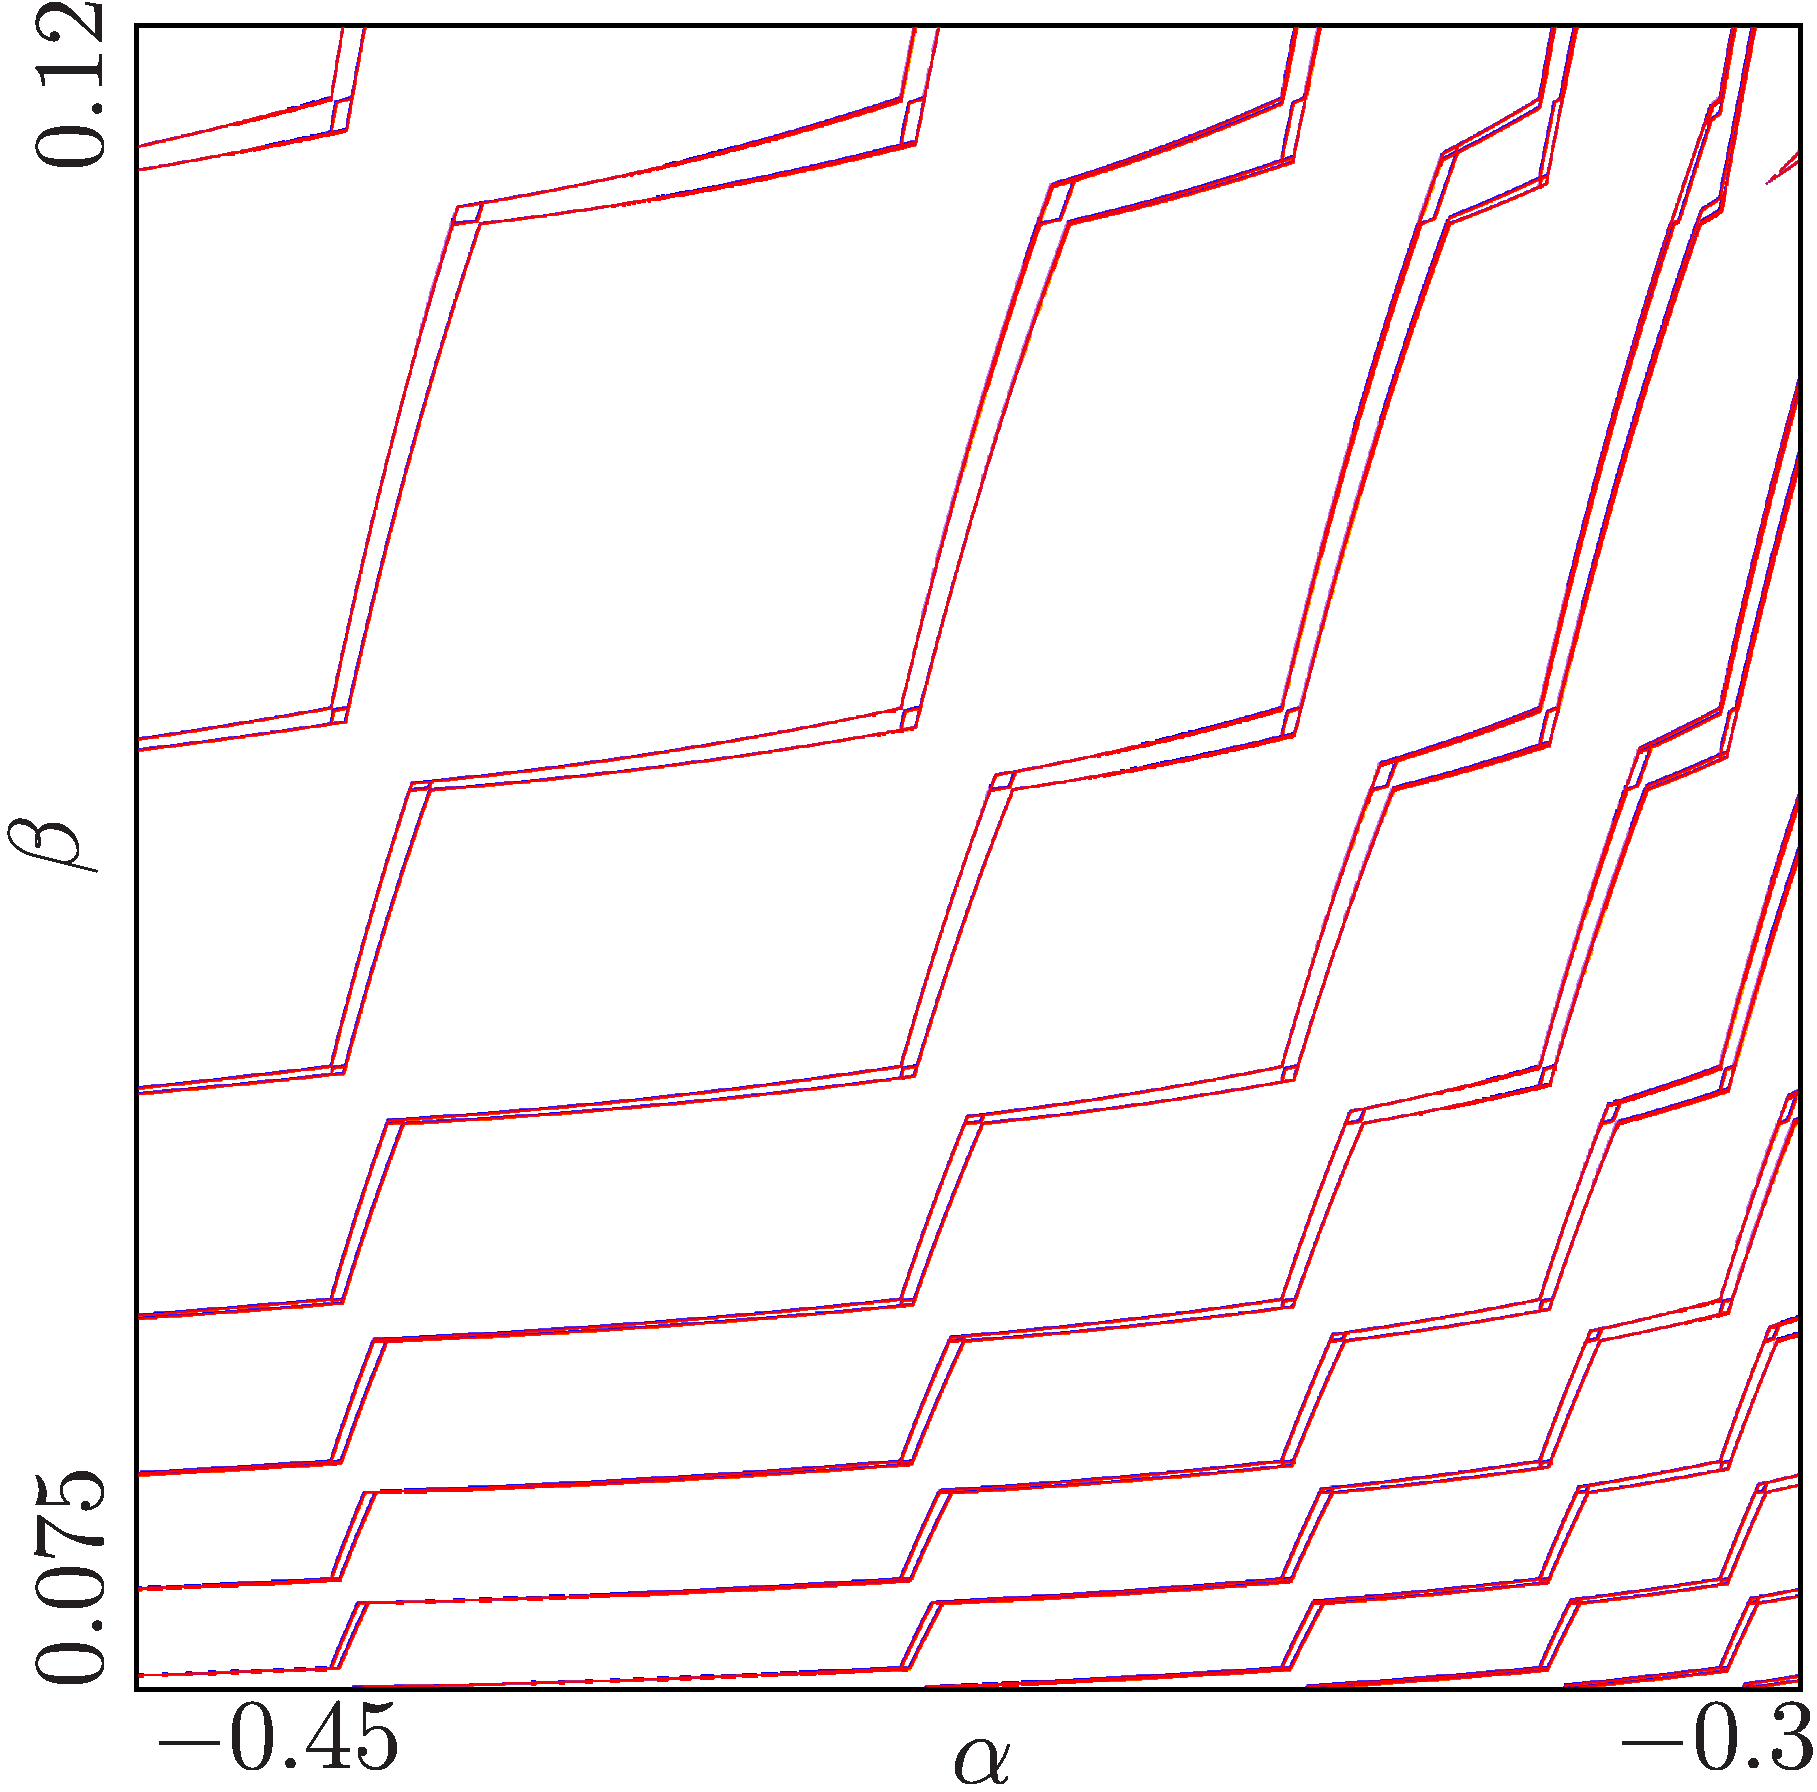
\includegraphics[width=.4 \textwidth]{Figs/archetypal_model_regions_drifting_apart.png}
			\quad
			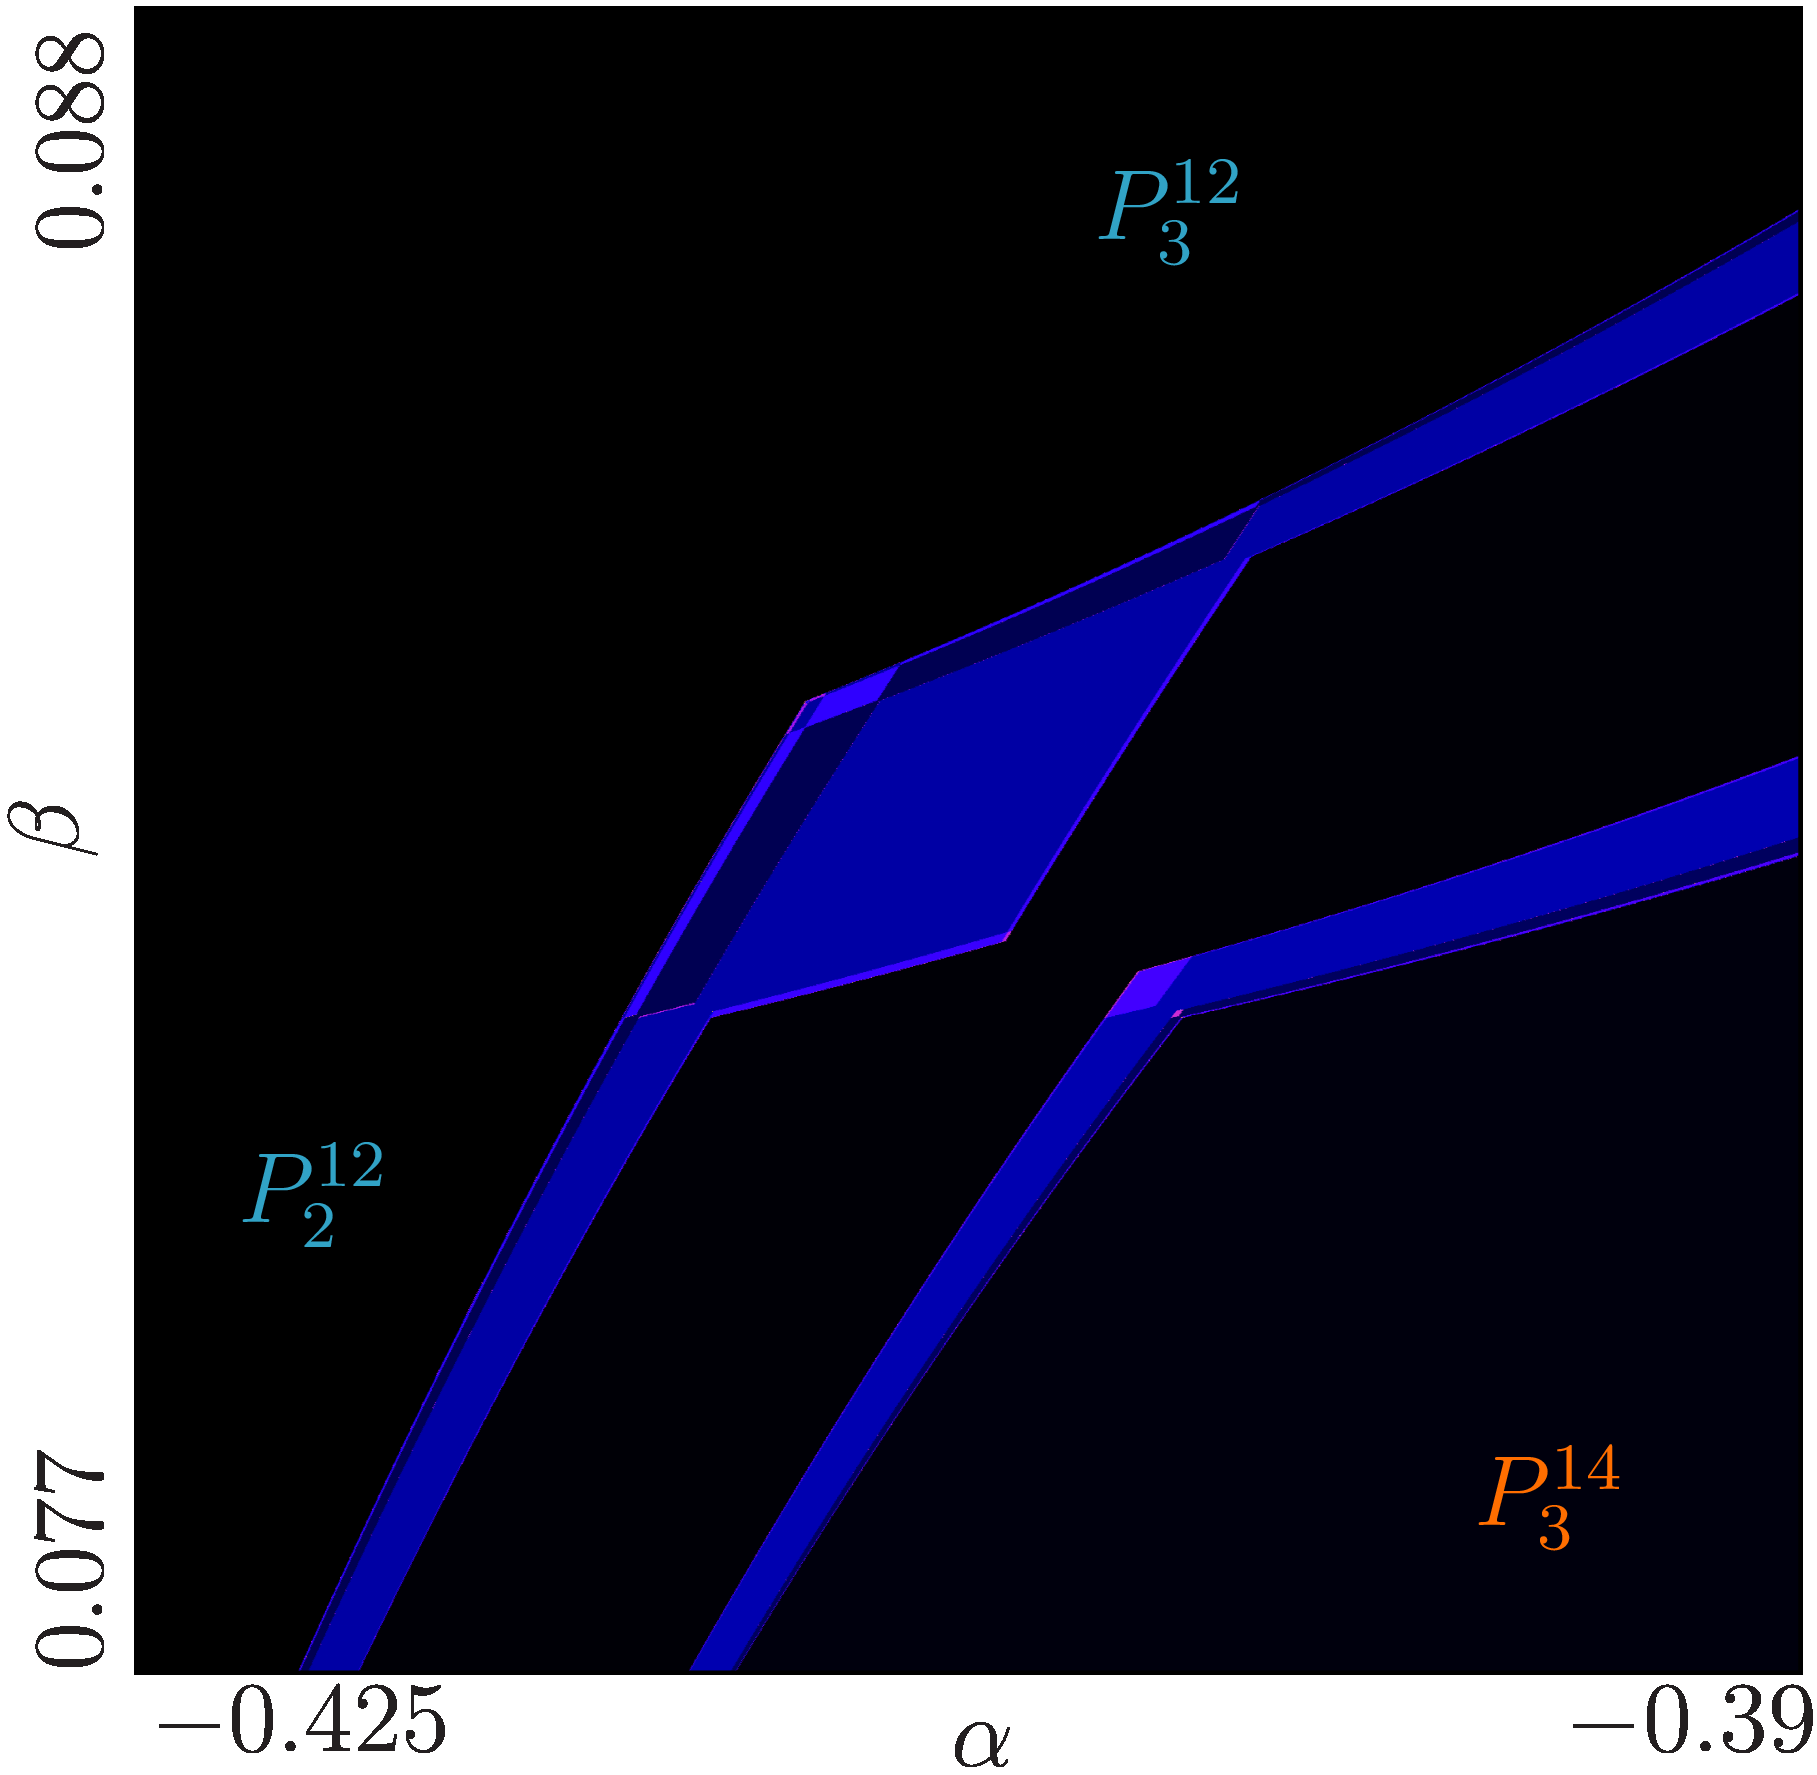
\includegraphics[width=.4 \textwidth]{Figs/archetypal_model_adding_like_period_corner.png}
		\end{figure}
	}
	\only<2>{
		\vspace{-1em}
		\begin{figure}
			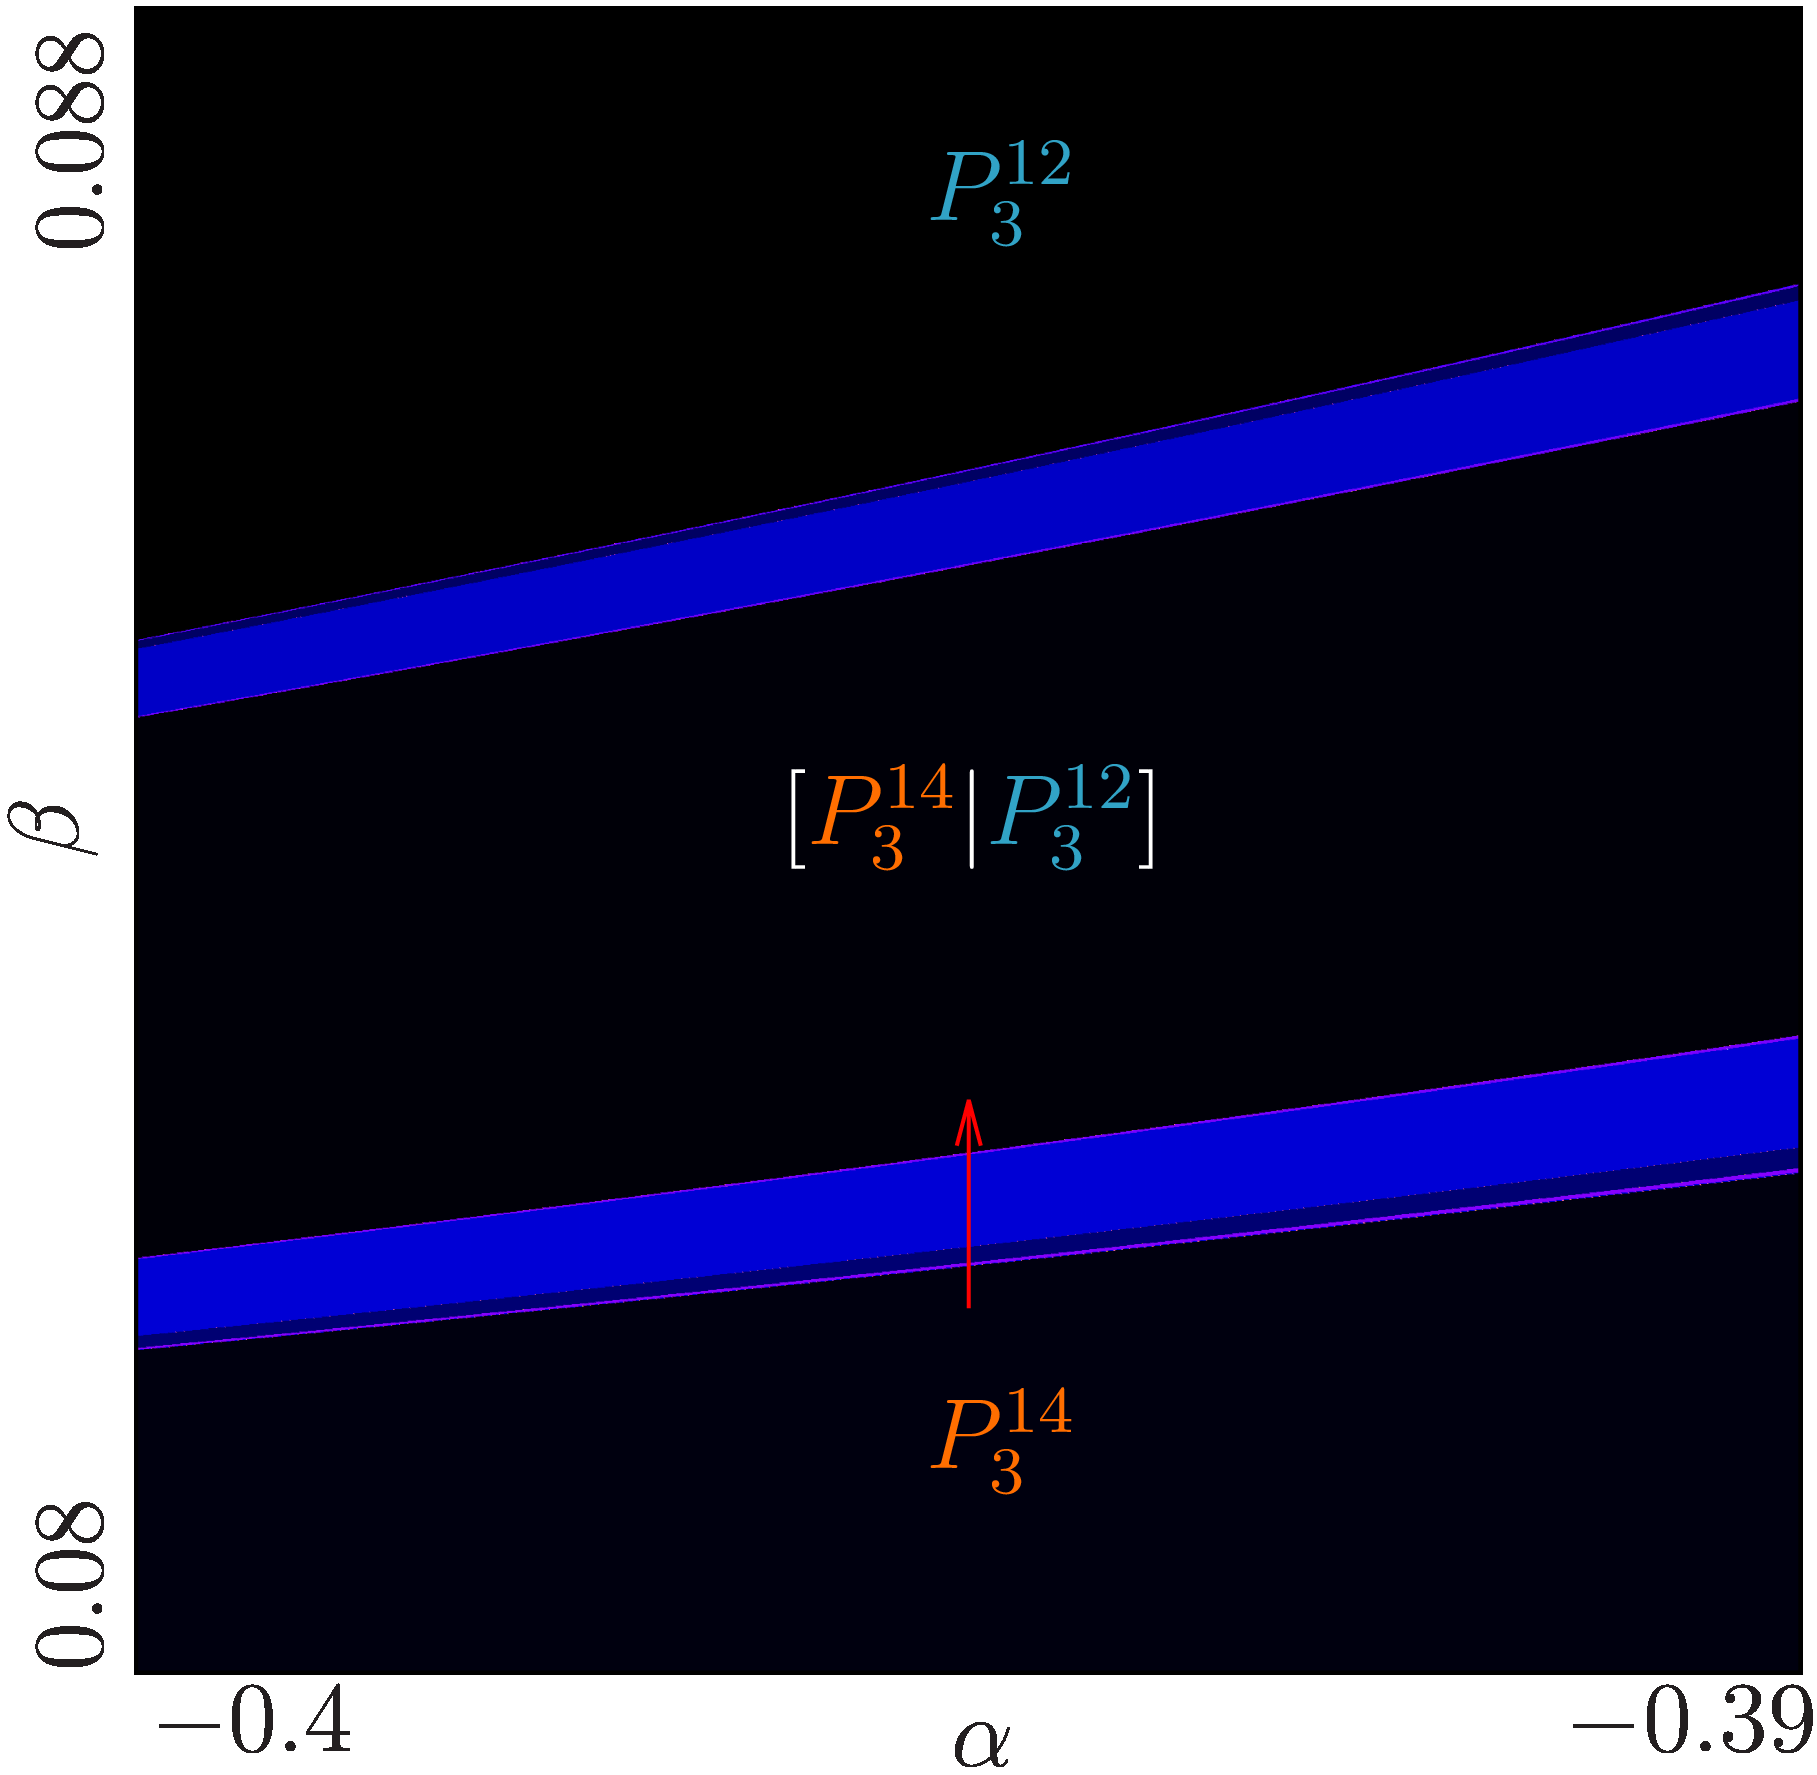
\includegraphics[width=.4 \textwidth]{Figs/archetypal_model_full_add_hor_2D.png}
			\qquad
			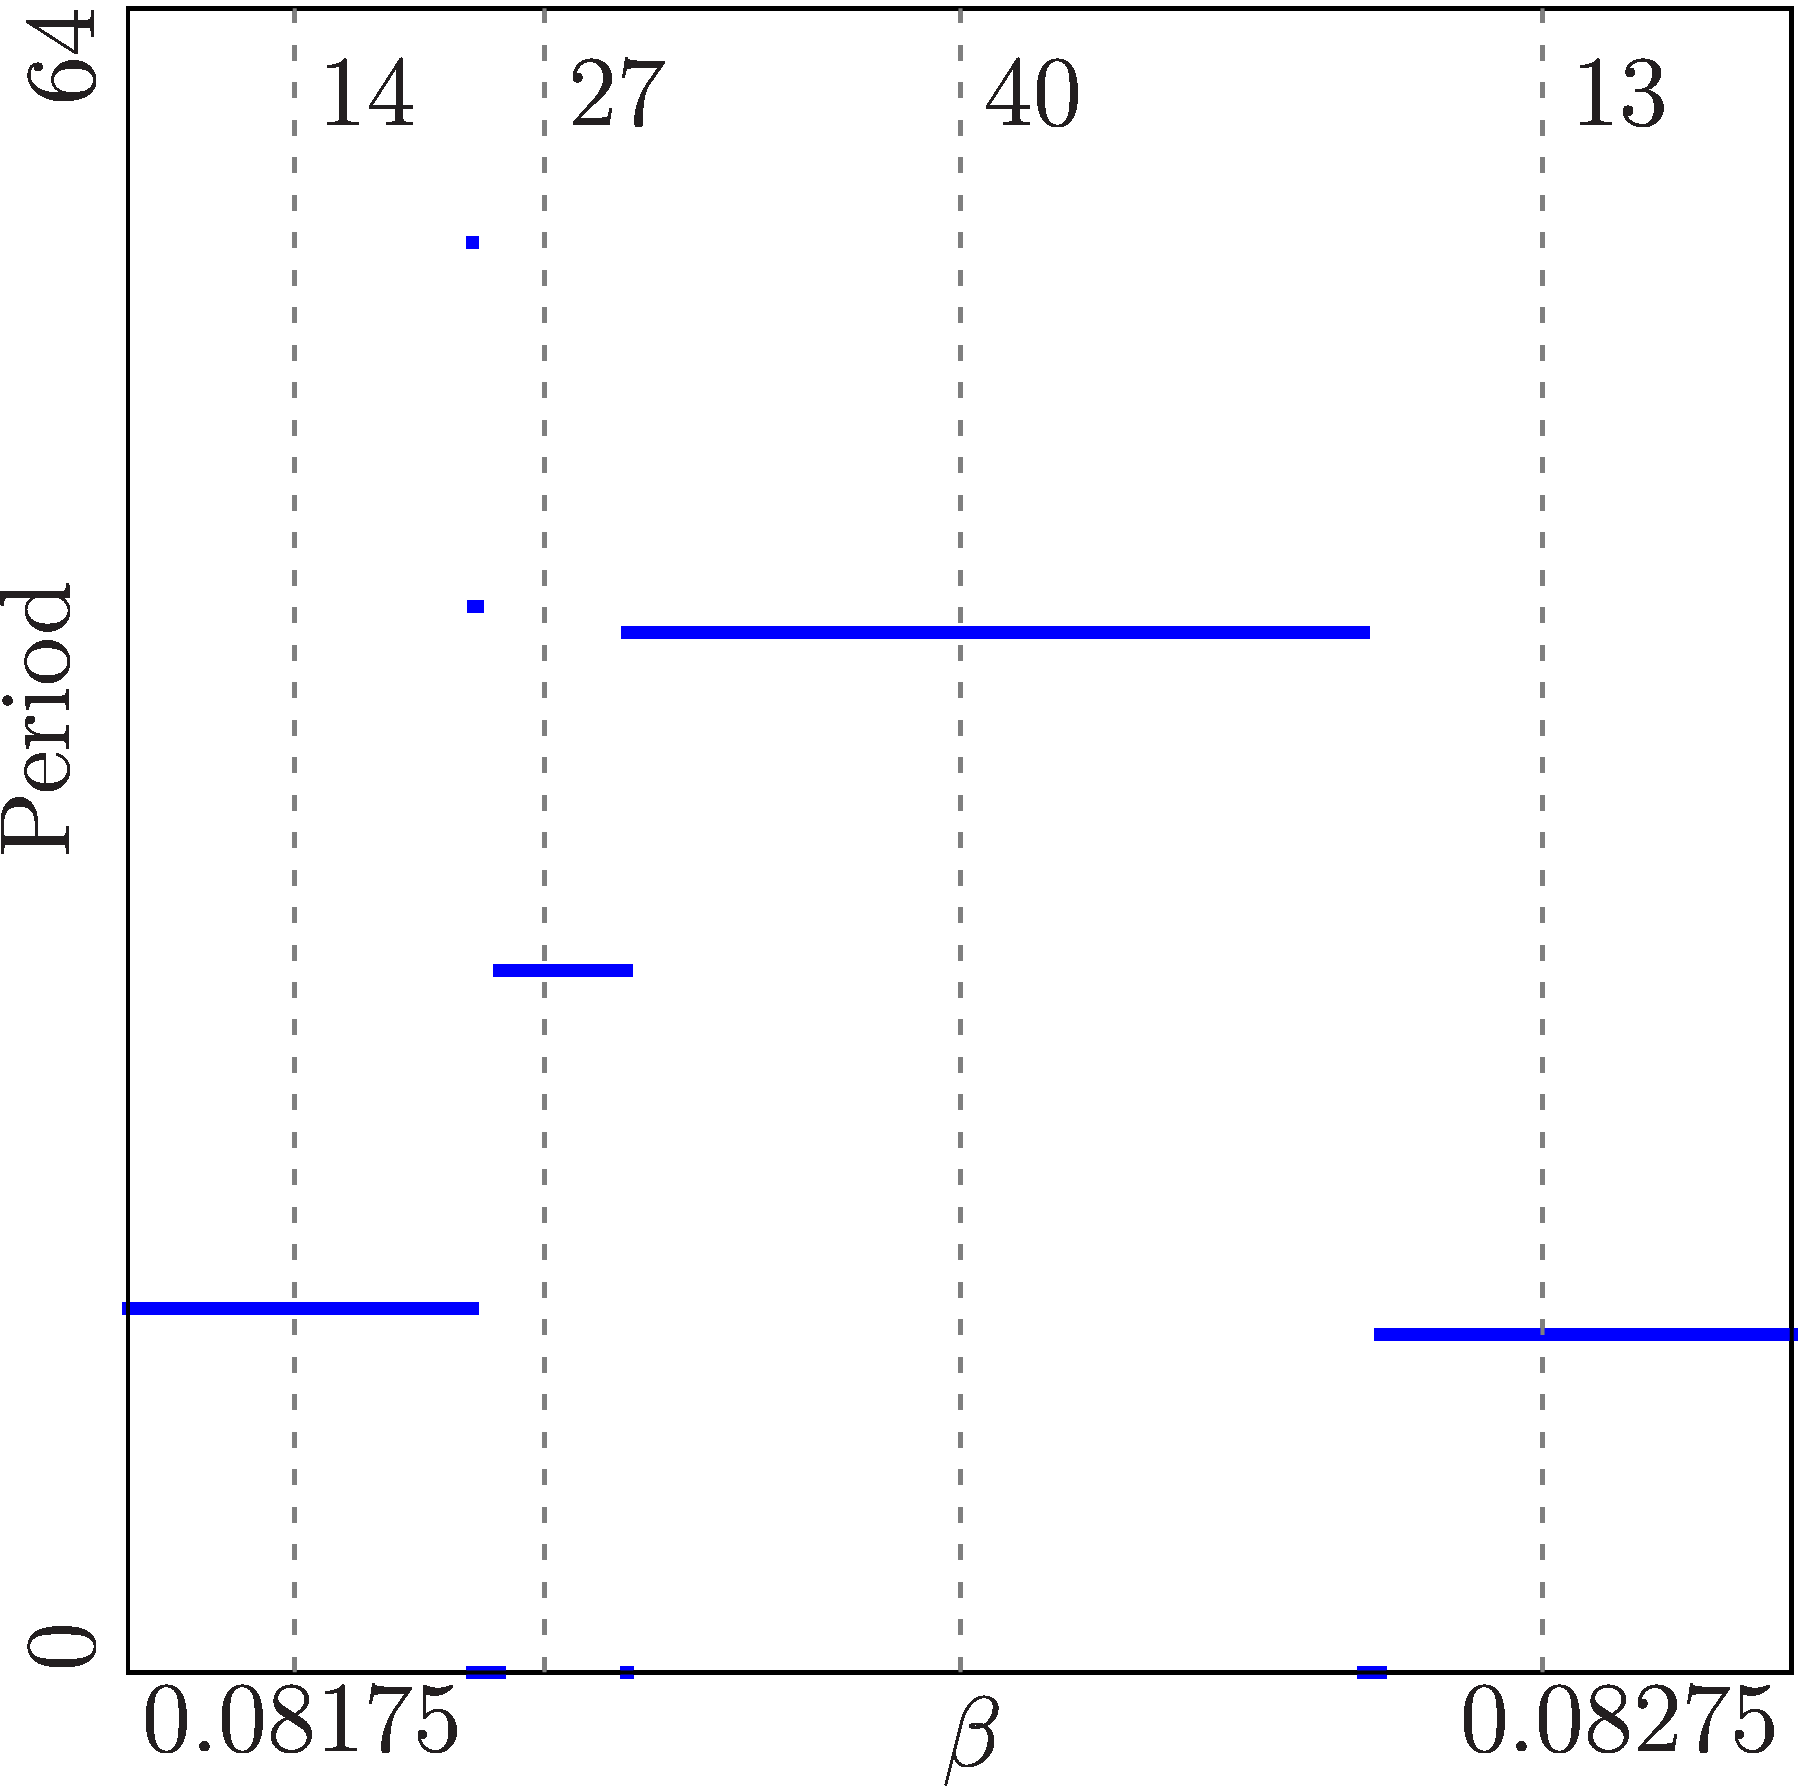
\includegraphics[width=.4 \textwidth]{Figs/archetypal_model_full_add_hor_1D.png}
		\end{figure}
	}
	\only<3>{
		\vspace{-1em}
		\begin{figure}
			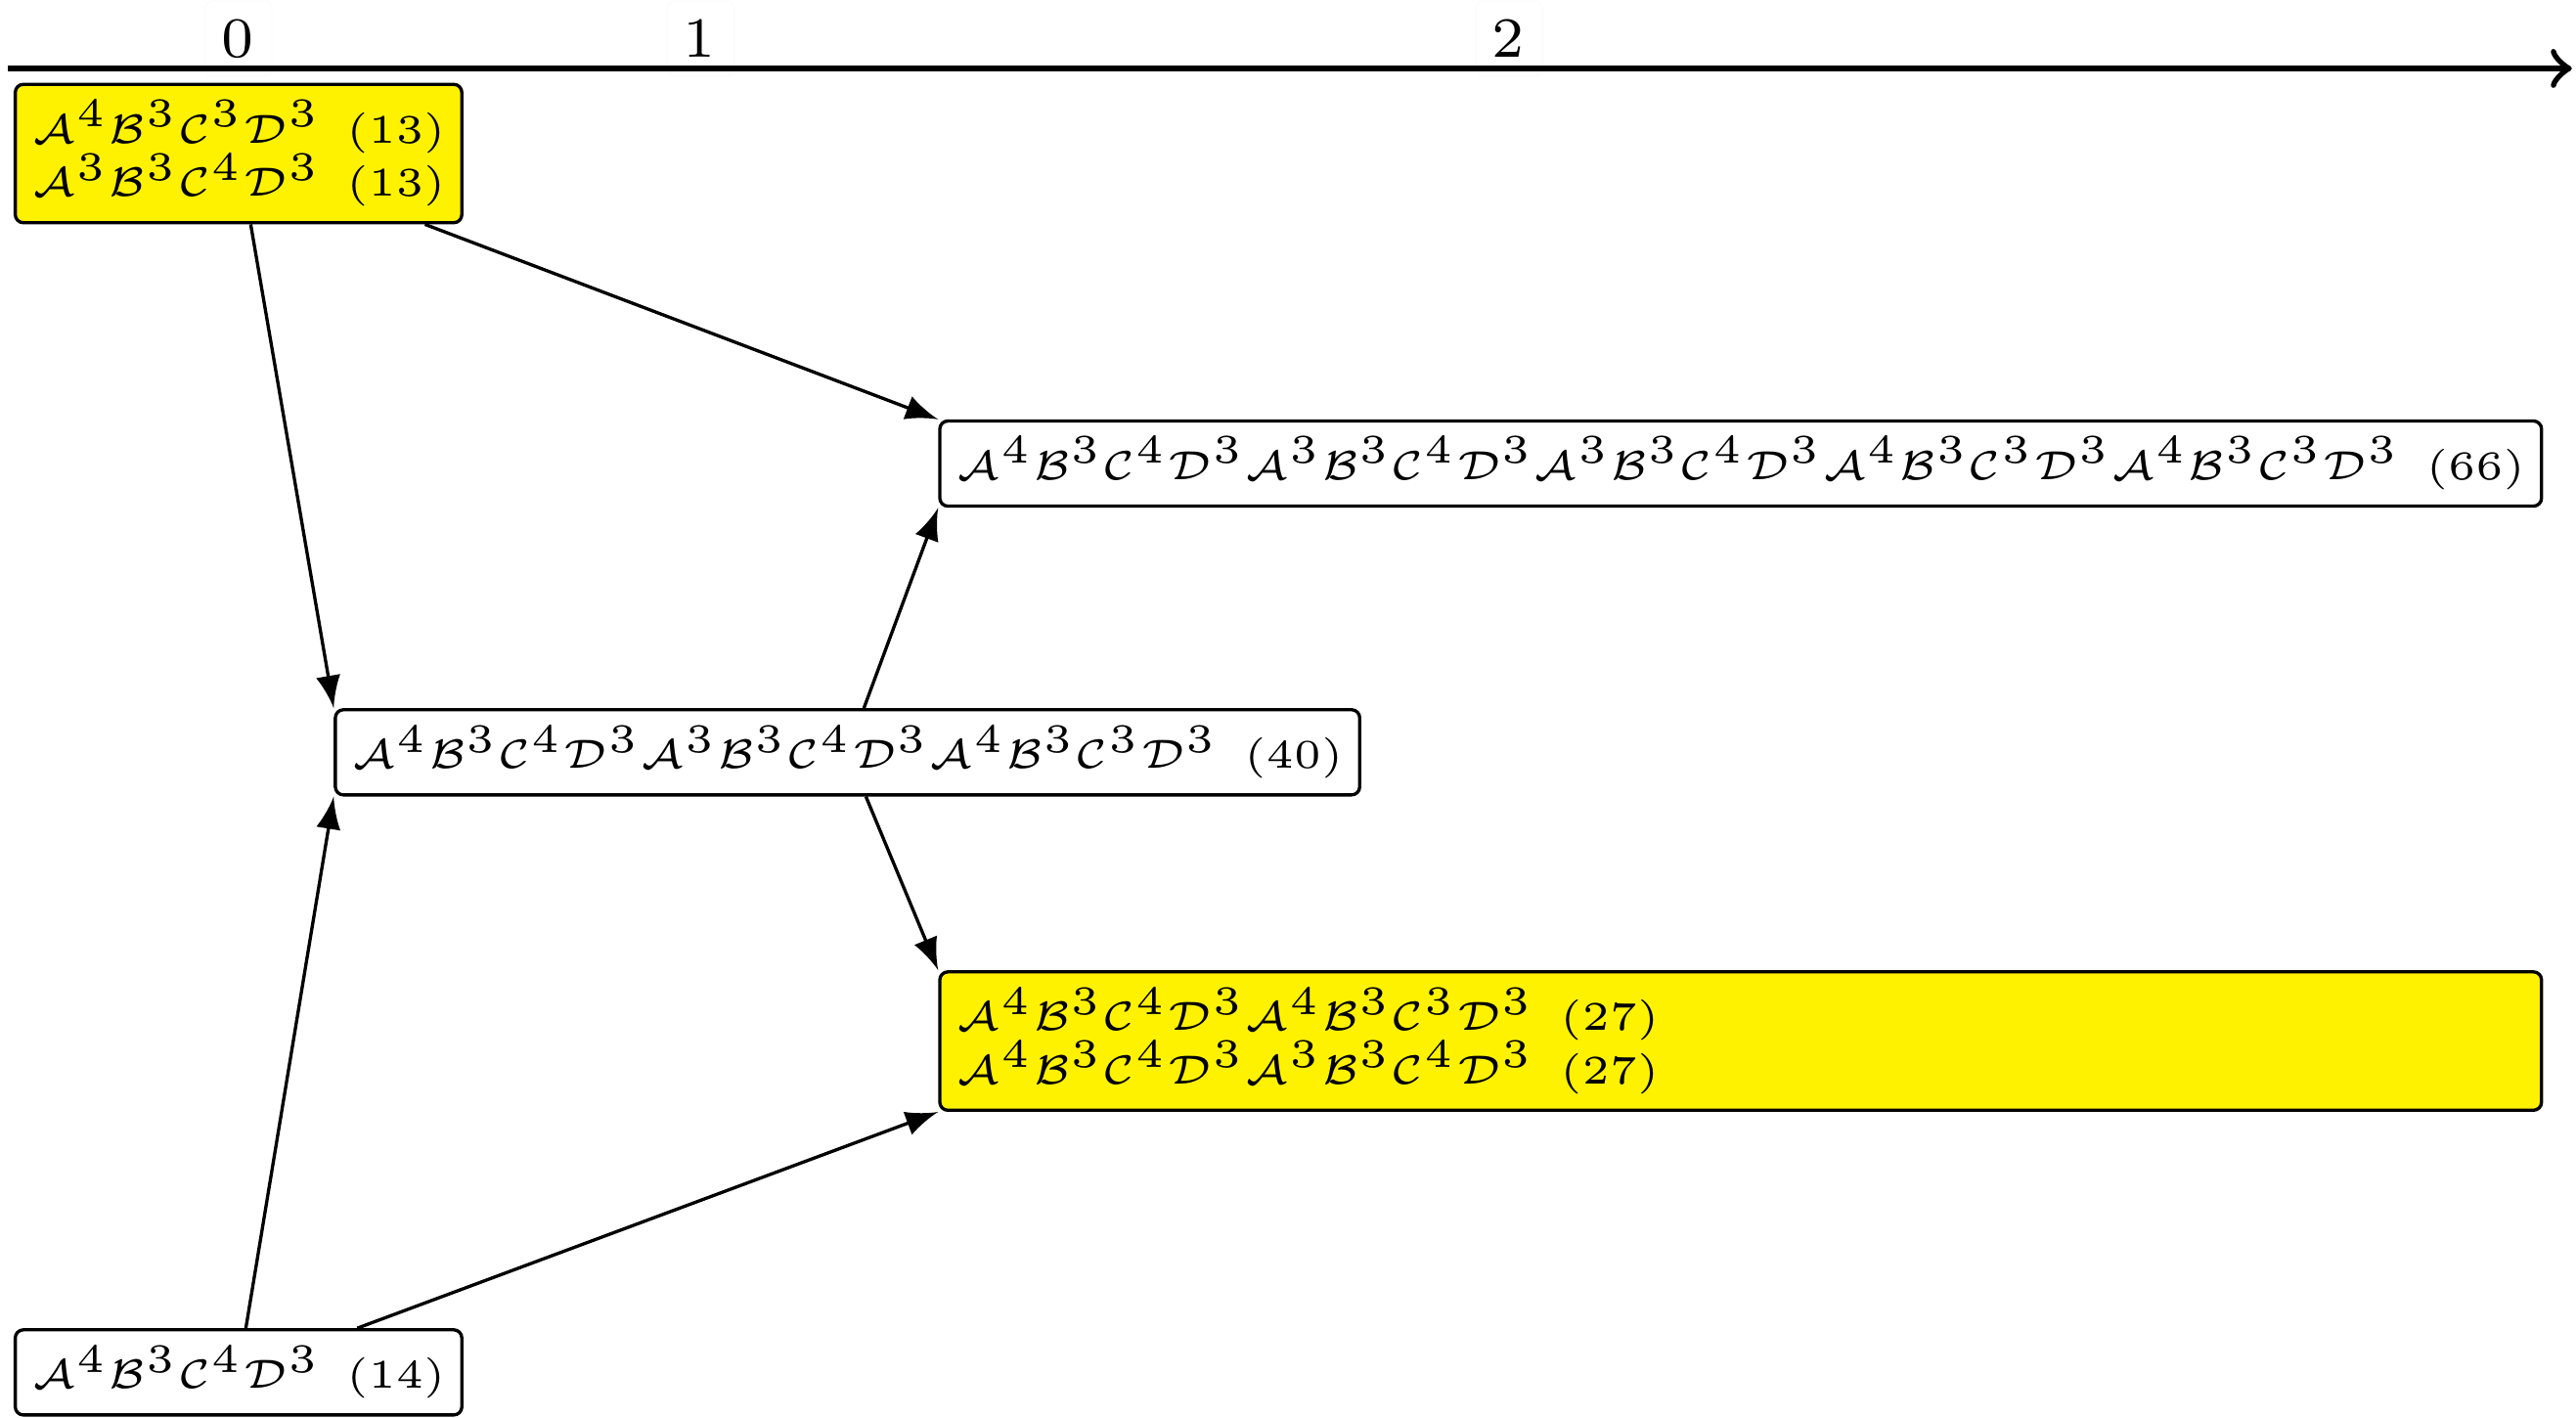
\includegraphics[width=.7 \textwidth]{Figs/Trees/FullArchetypal/adding.png}
		\end{figure}
	}
\end{frame}

\begin{frame}{Halved Model}
	\vspace{-1em}
	\begin{columns}
		\begin{column}{.4 \textwidth}
			\begin{figure}
				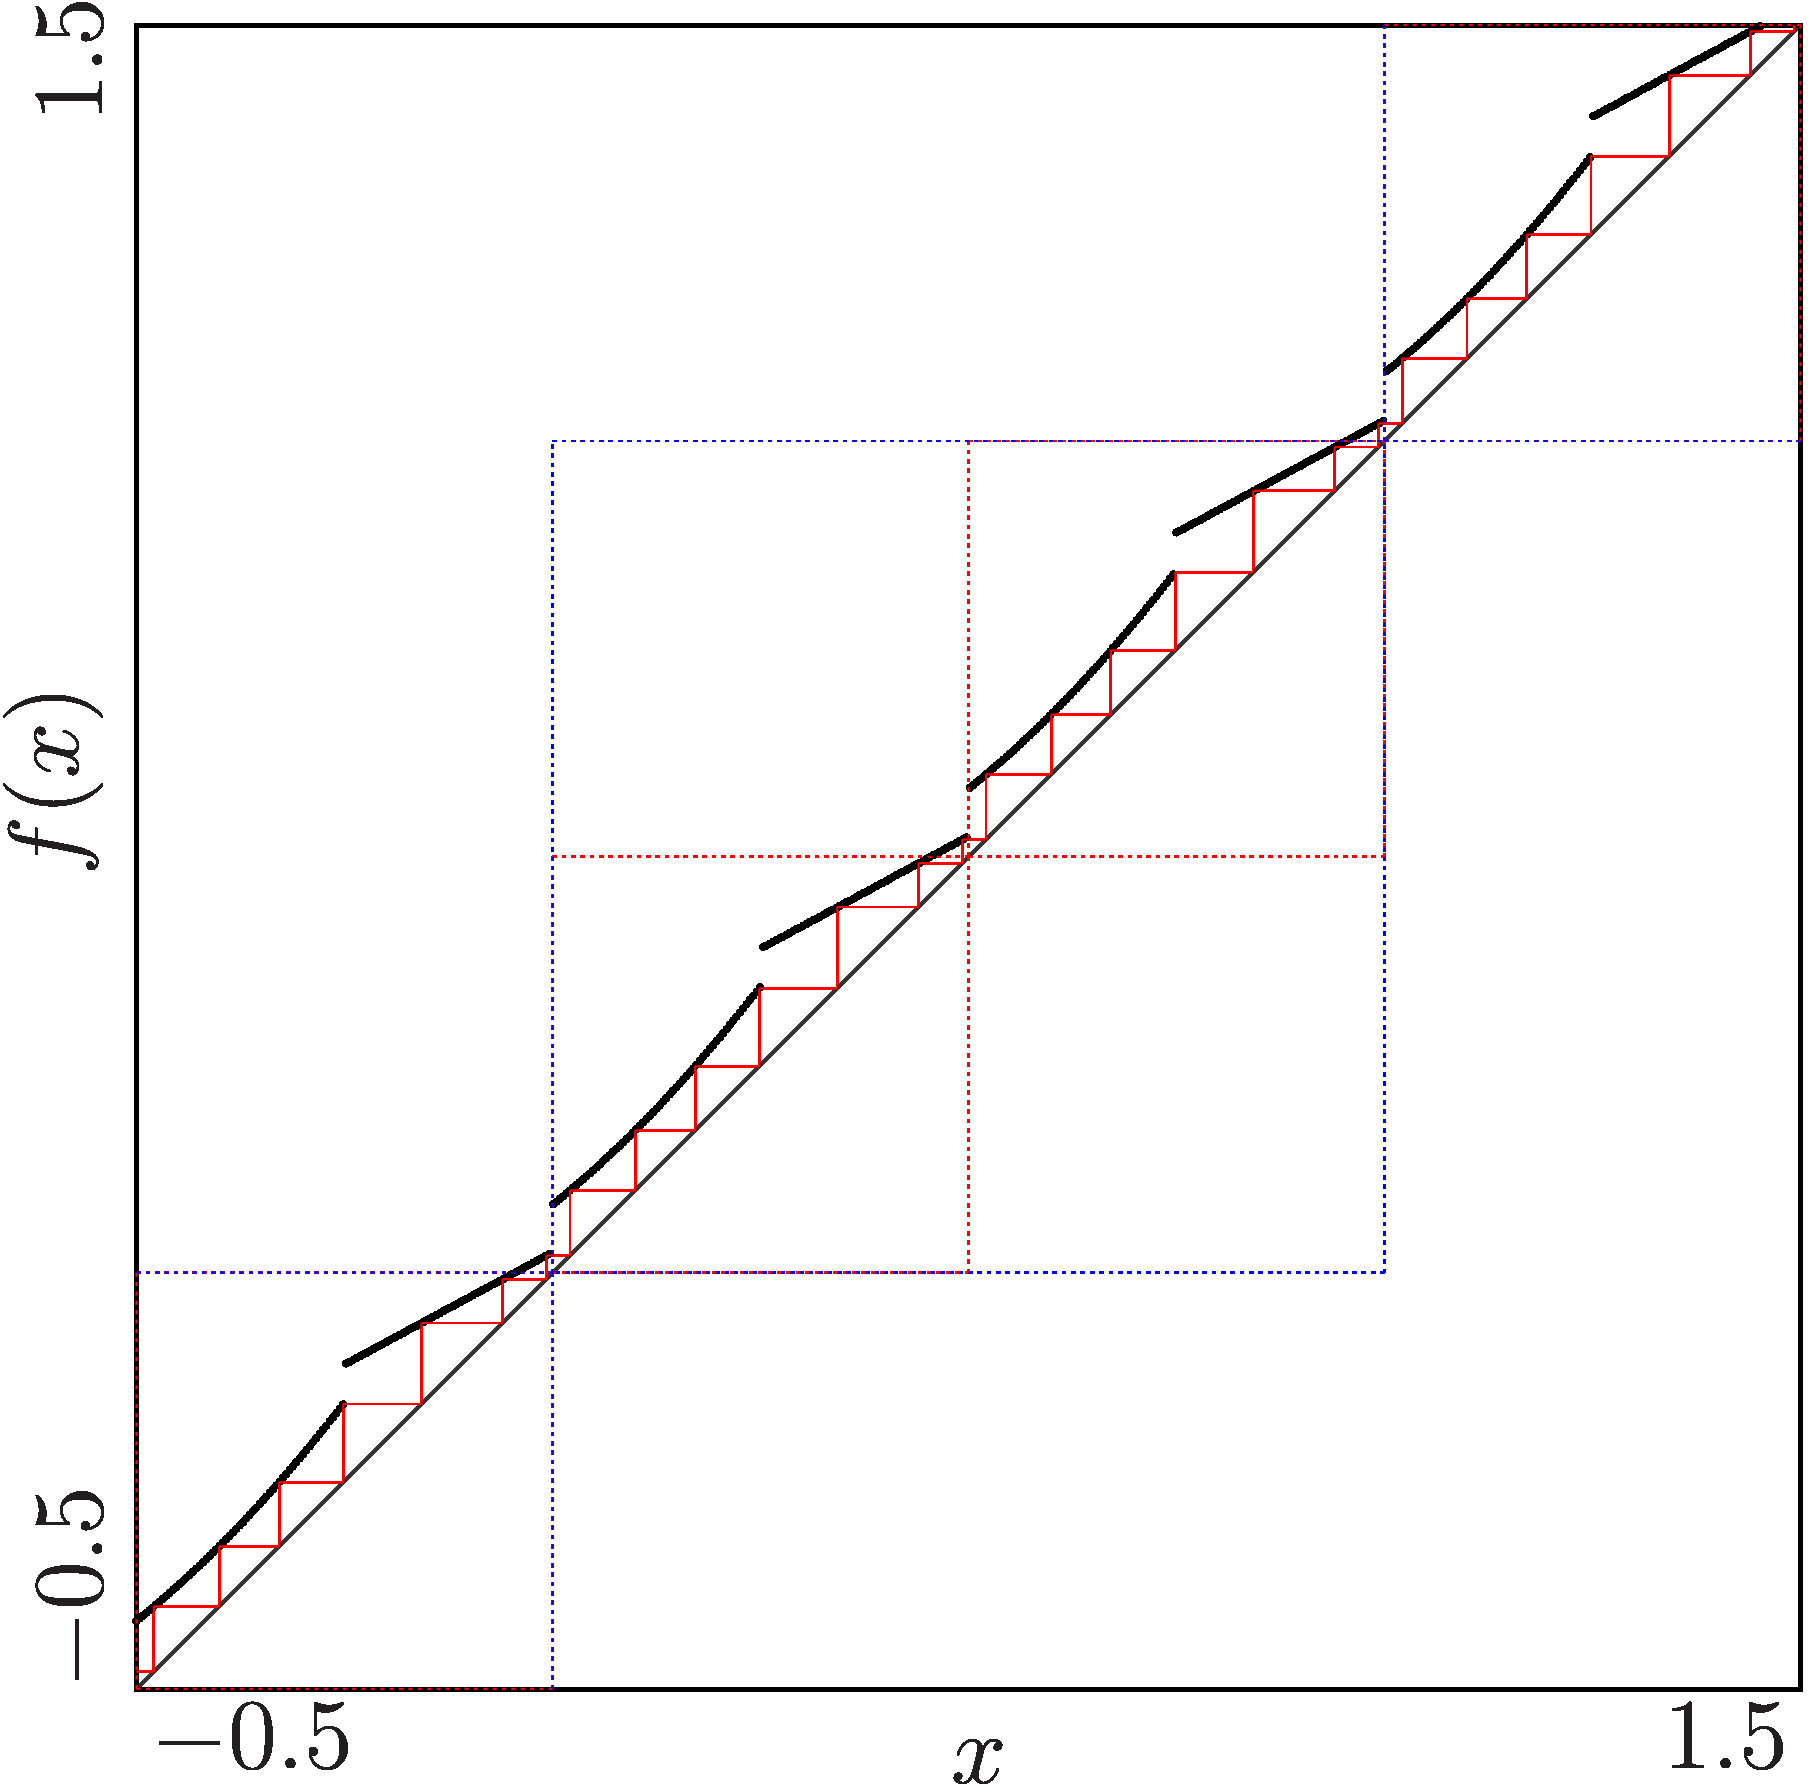
\includegraphics[width=\textwidth]{Figs/archetypal_model_lifted.png}
			\end{figure}
		\end{column}
		\begin{column}{.5 \textwidth}
			\begin{itemize}
				\item Lift the model from $[0, 1)$ to $\mathbb{R}$
				      %\item The lifted model repeats every $1$ step
				      %\item But it even repeats every $\frac{1}{2}$ step because of the built-in symmetry
				\item Drop the model to $[0, \frac{1}{2})$
				\item[$\Rightarrow$] Halved Model
			\end{itemize}
			\begin{align*}
				x    & \mapsto g(x) \mod \frac{1}{2}                                              \\
				g(x) & = \begin{cases}
					         g_L(x) = a_L \cdot x^2 + b_L \cdot x + c_L & \text{ if } x < \frac{1}{4} \\
					         g_R(x) = b_R \cdot x + c_R                 & \text{ else}
				         \end{cases}
			\end{align*}
		\end{column}
	\end{columns}
\end{frame}

\begin{frame}{Period Adding}
	\only<1>{
		\vspace{-1em}
		\begin{figure}
			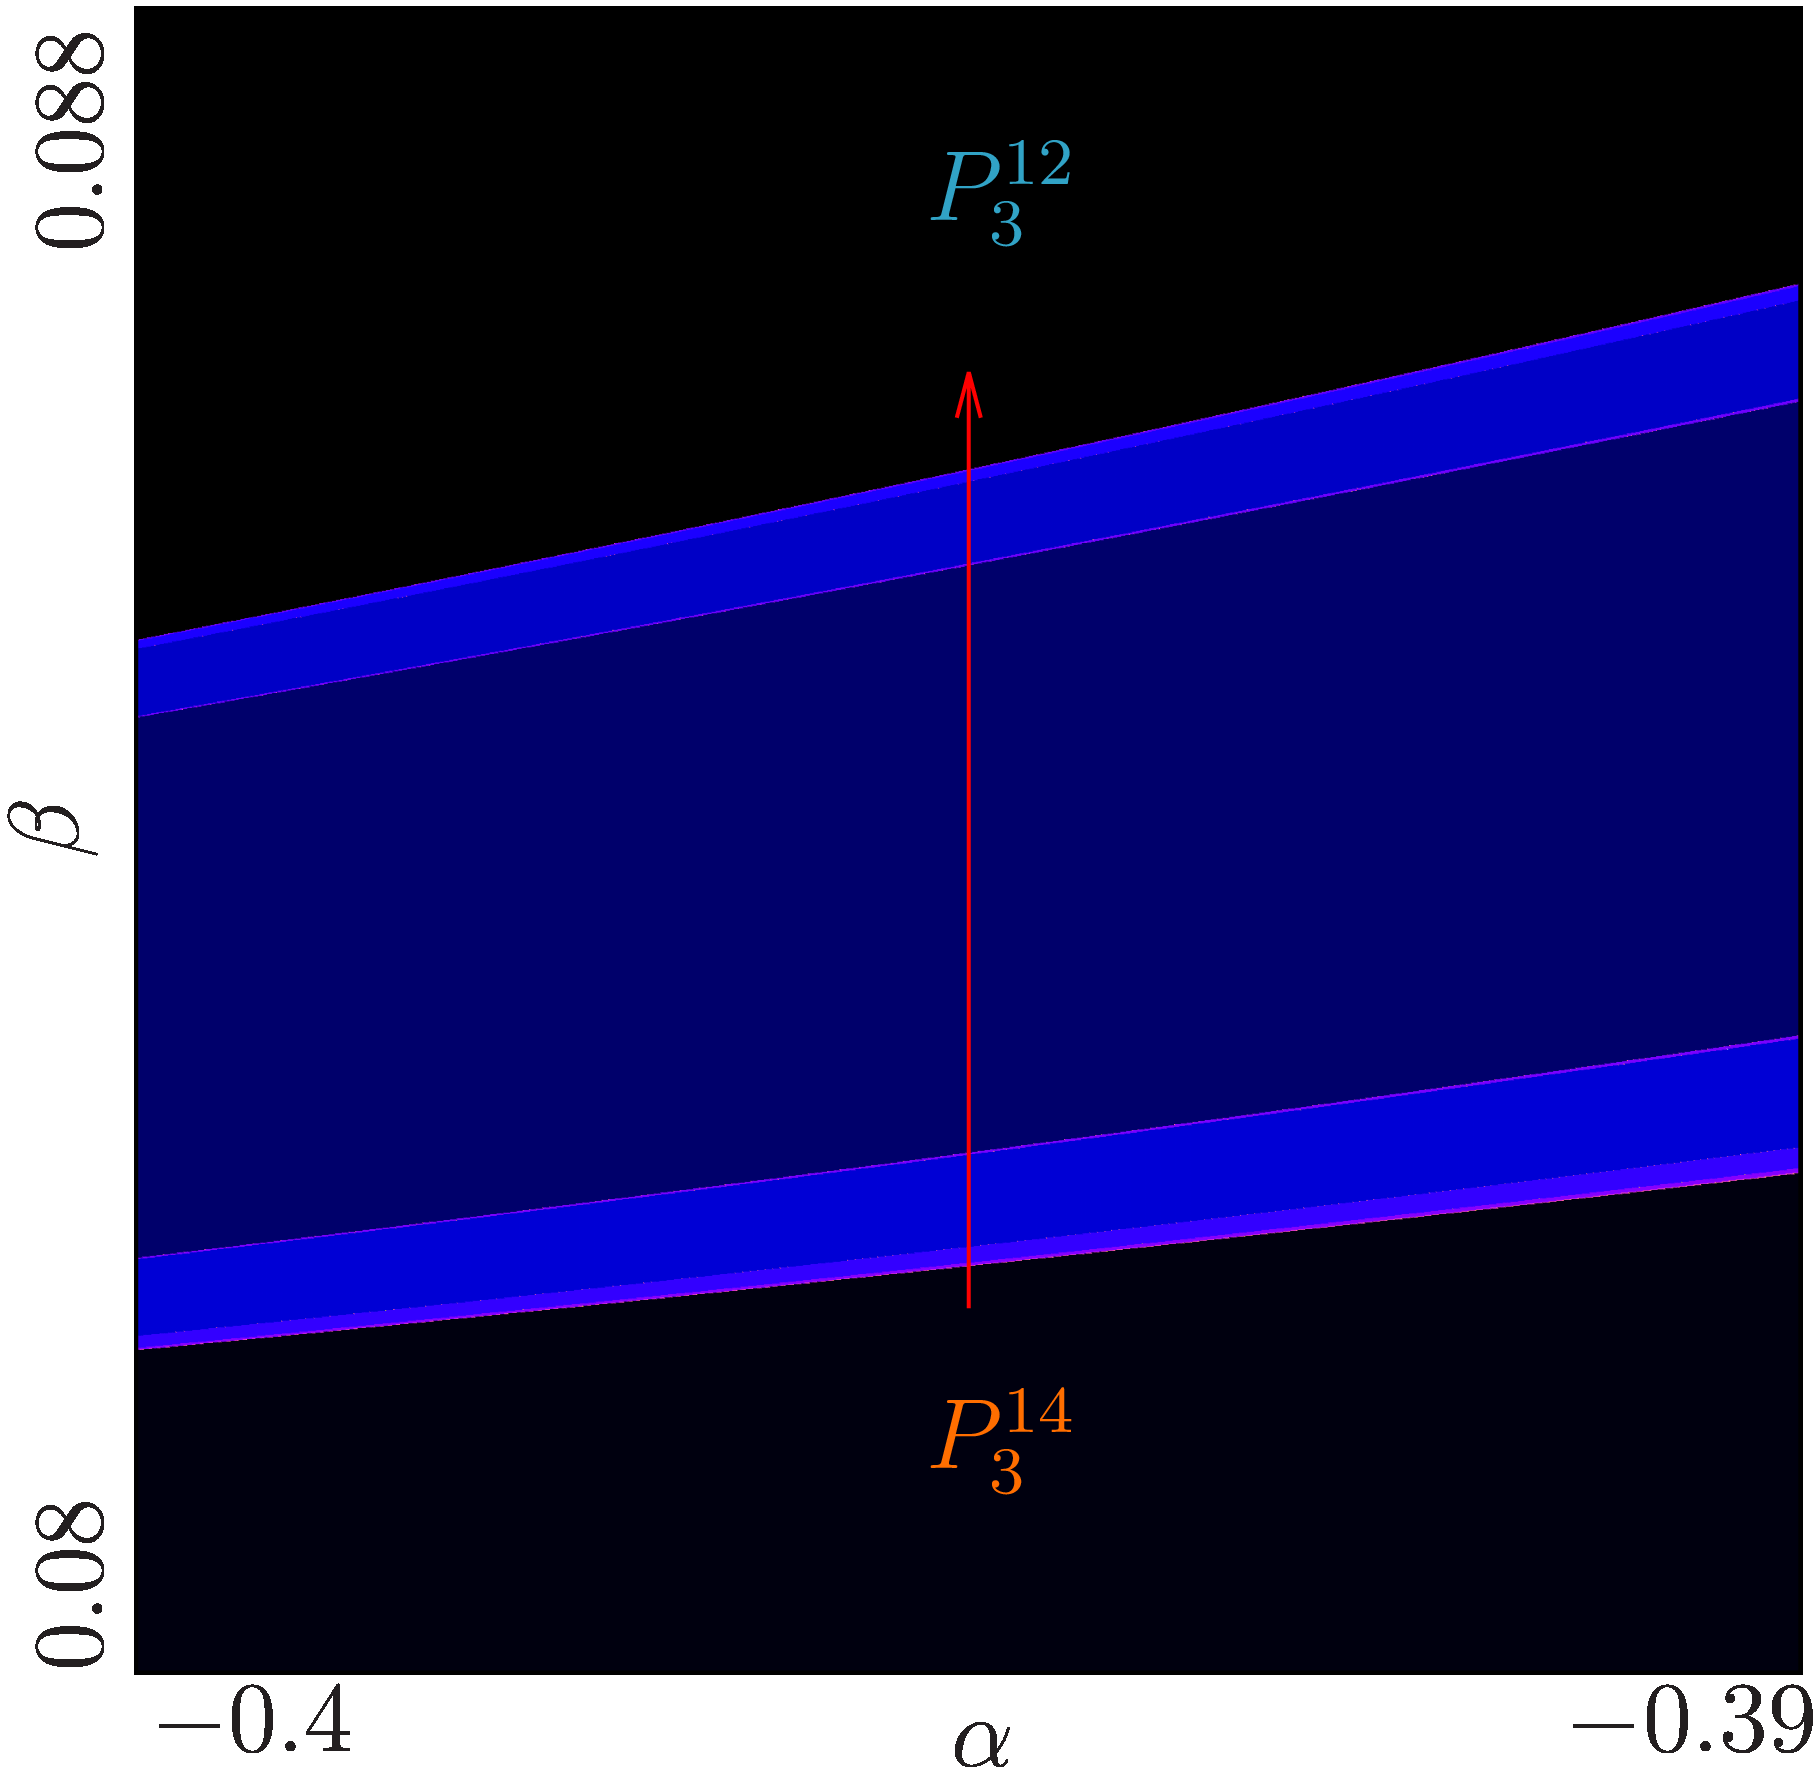
\includegraphics[width=.4 \textwidth]{Figs/archetypal_model_halved_add_hor_2D.png}
			\quad
			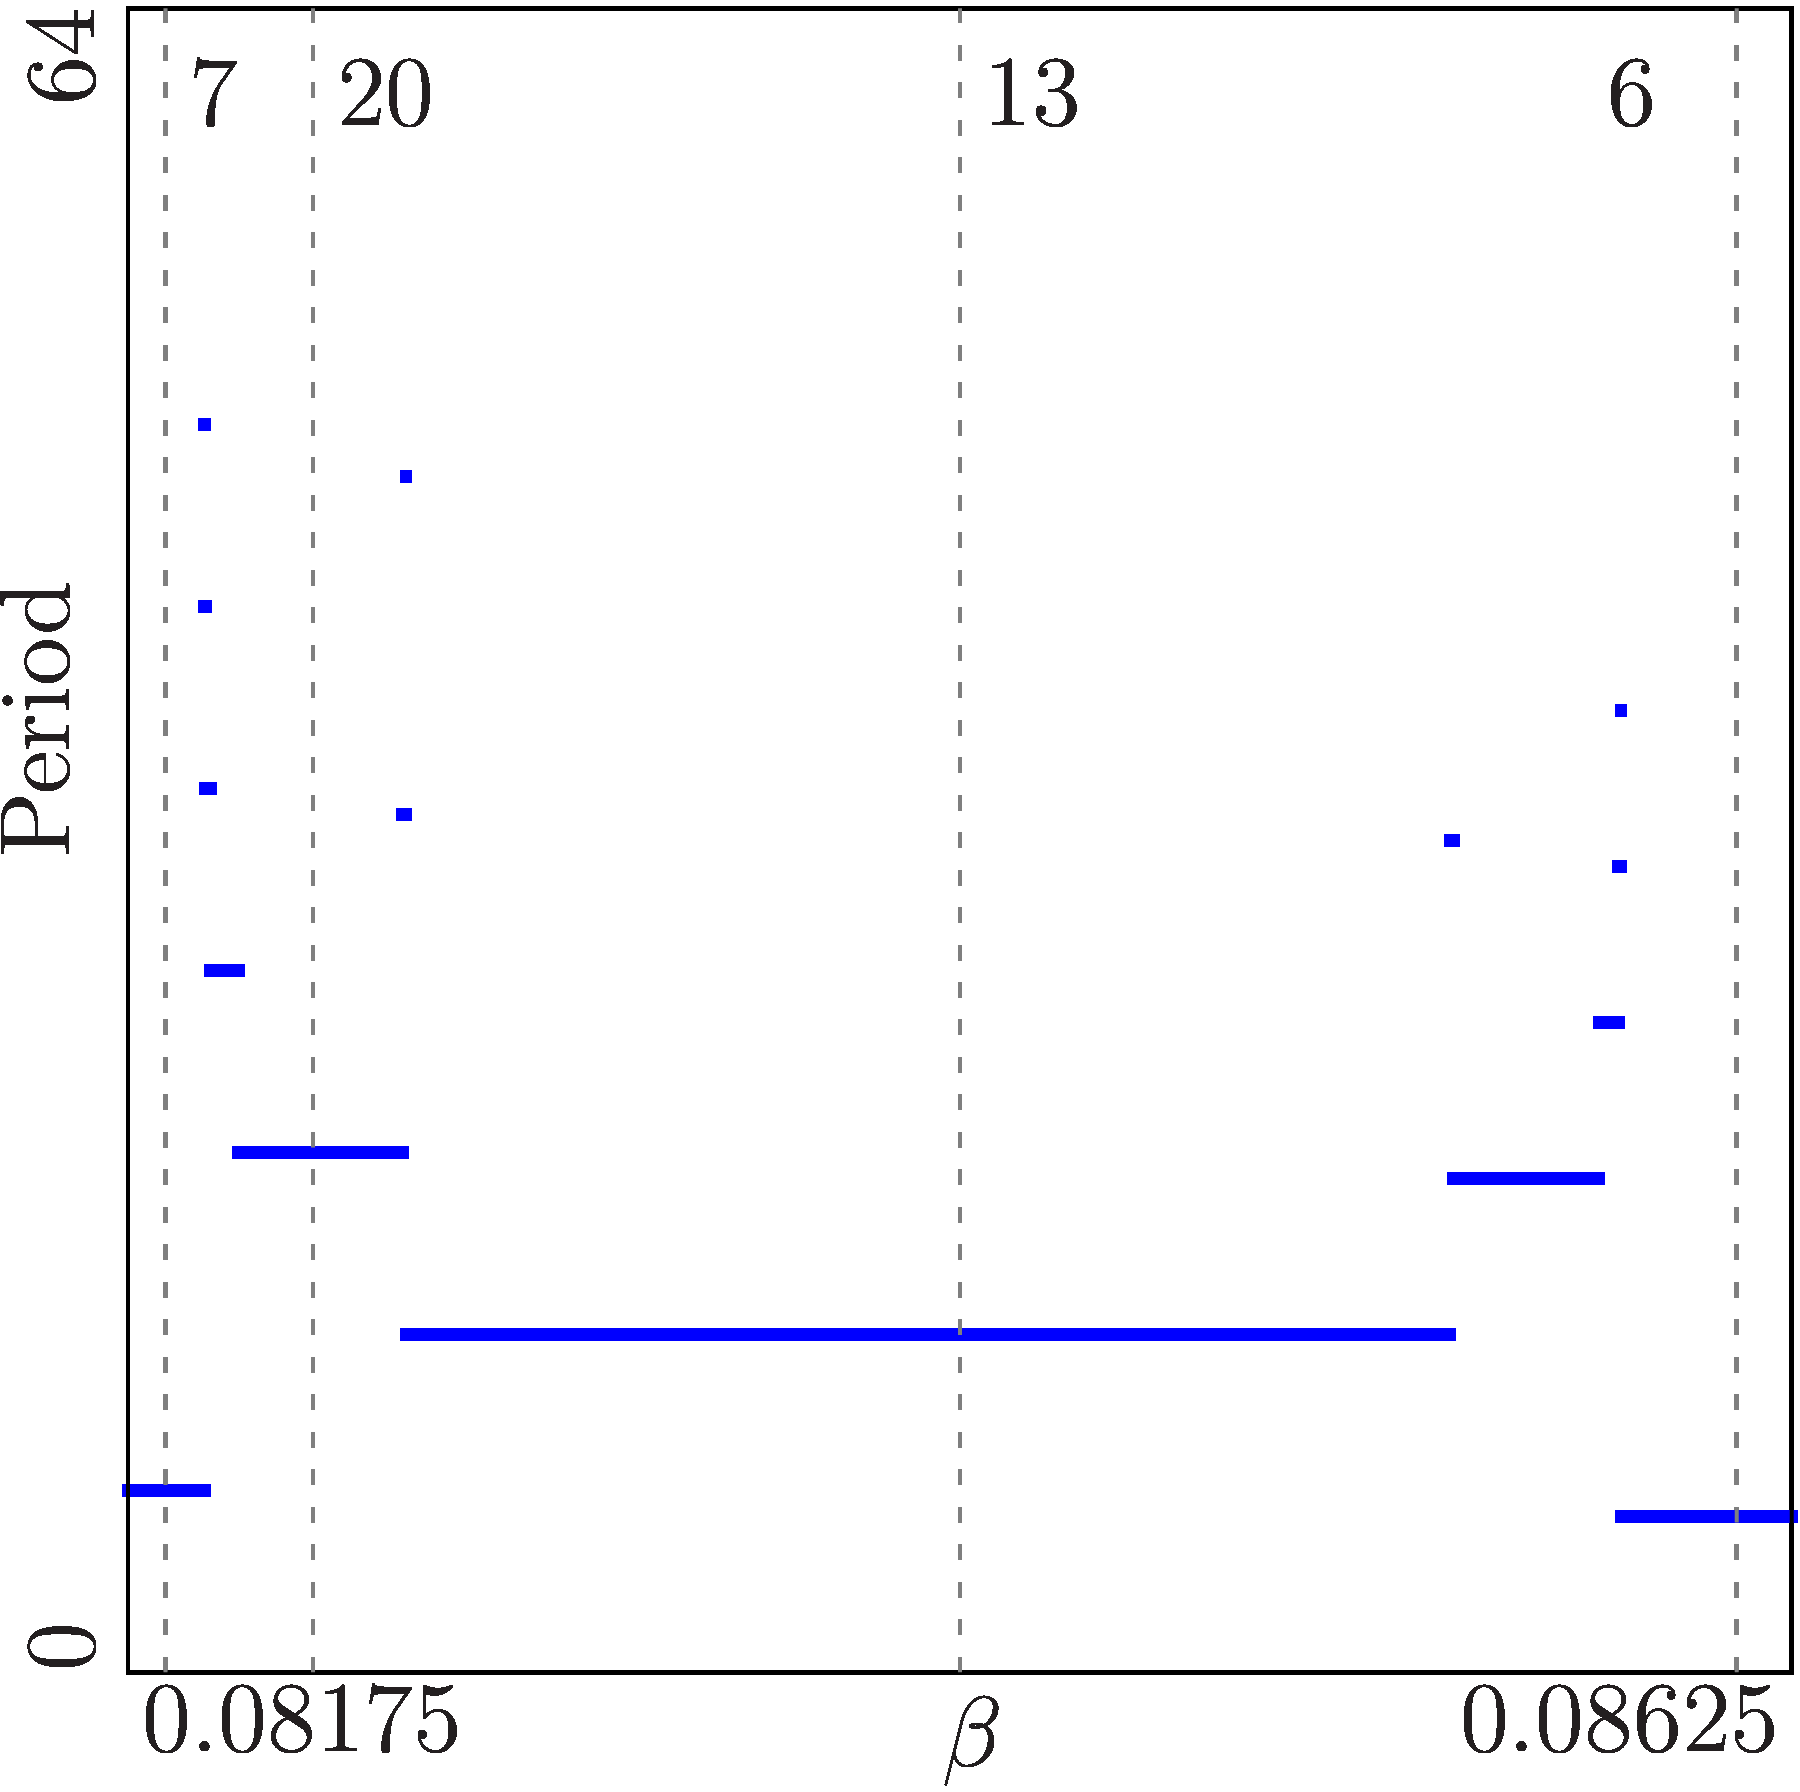
\includegraphics[width=.4 \textwidth]{Figs/archetypal_model_halved_add_hor_1D.png}
		\end{figure}
	}
	\only<2>{
		\vspace{-1em}
		\begin{figure}
			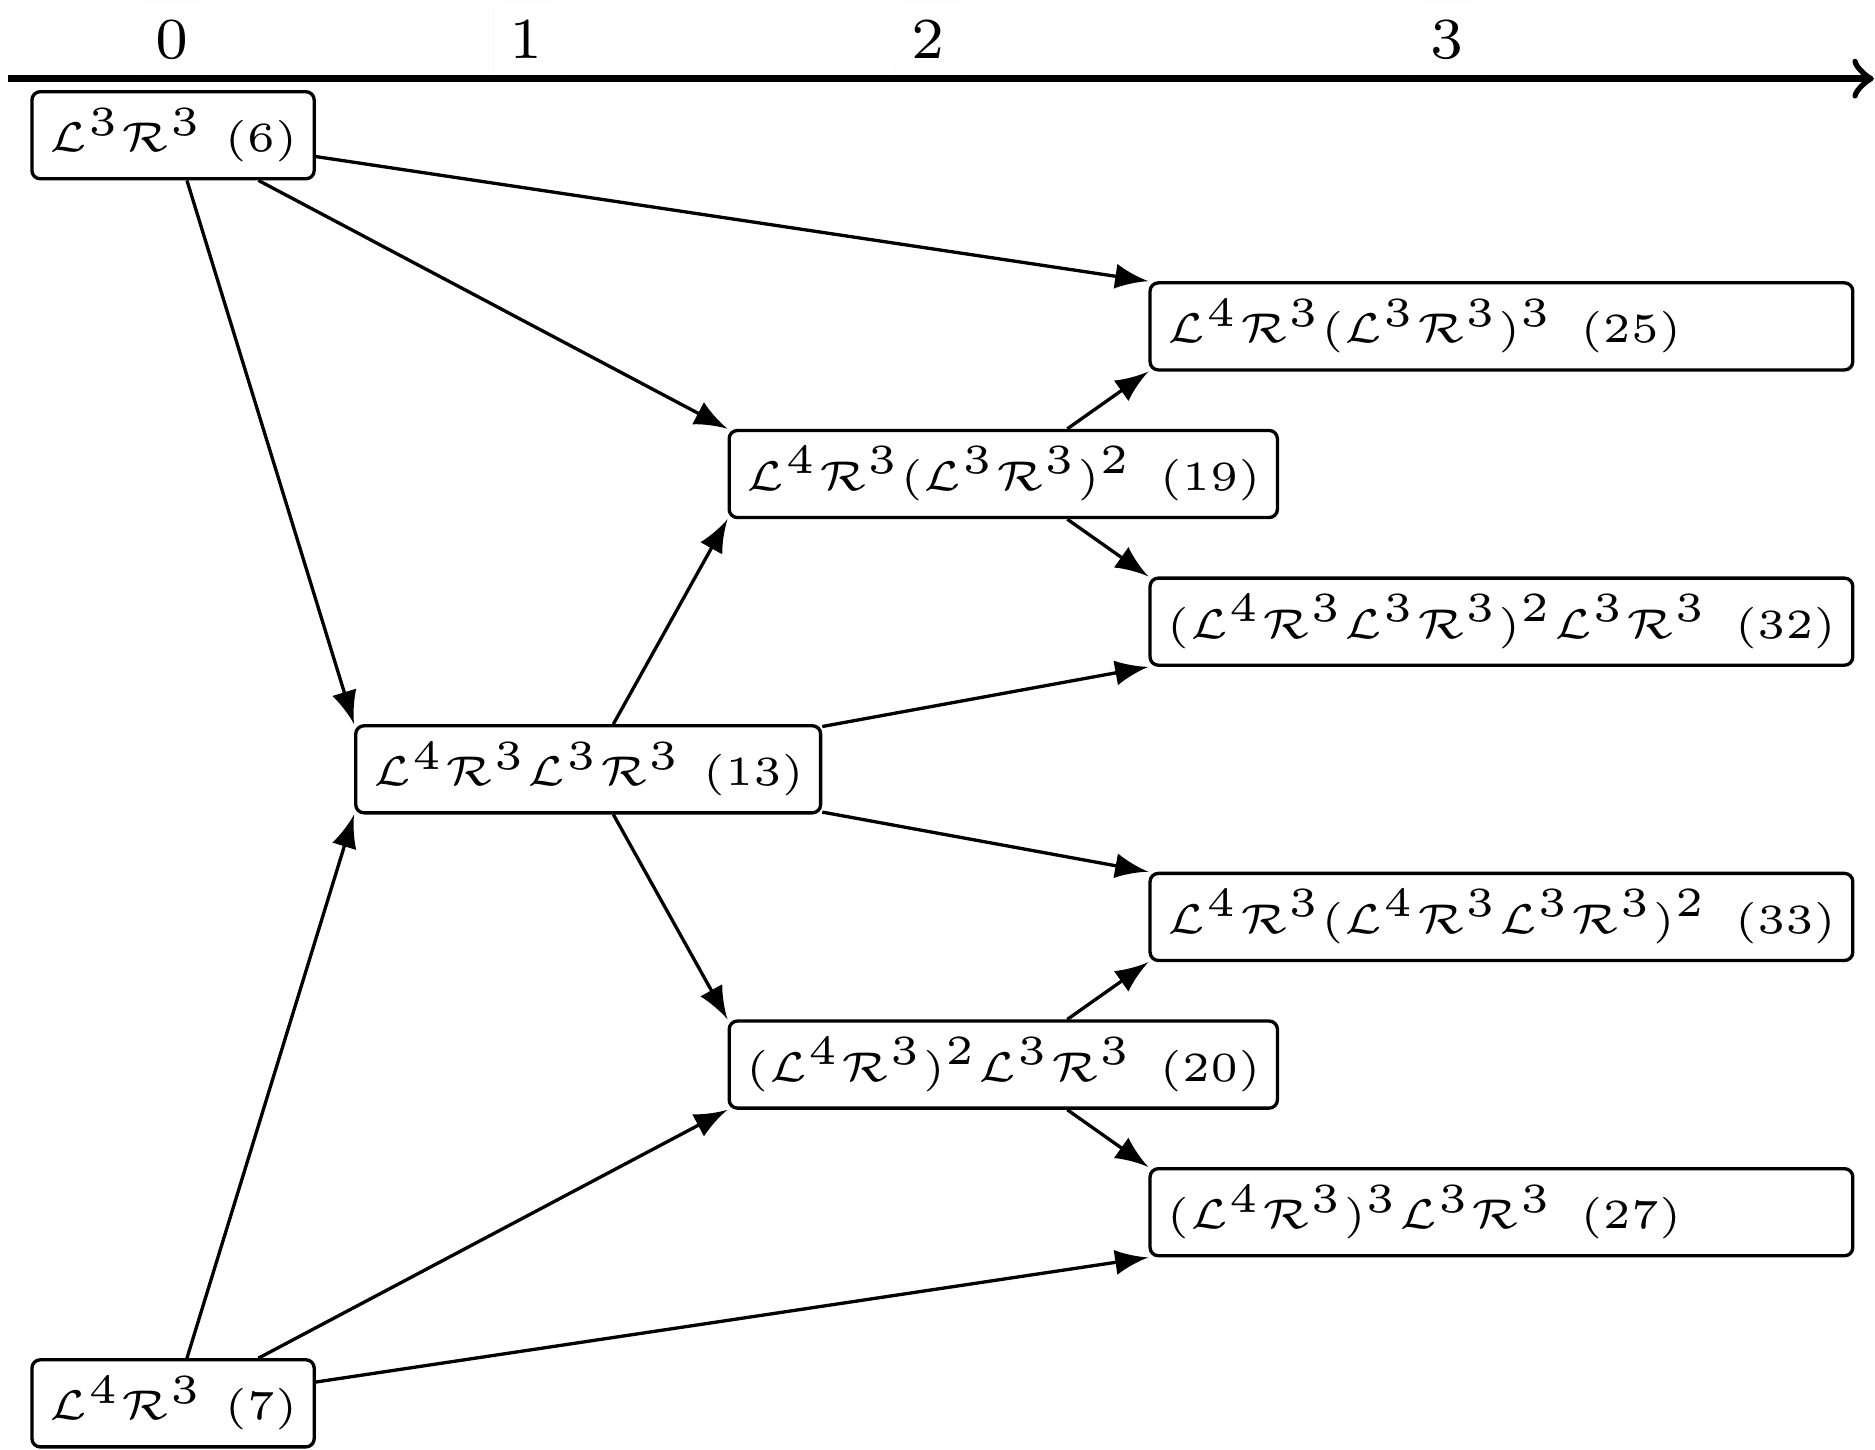
\includegraphics[width=.6 \textwidth]{Figs/Trees/HalvedArchetypal/adding.png}
		\end{figure}
	}
\end{frame}

\begin{frame}{Period Adding Results}
	\vspace{-1em}
	\begin{center}
		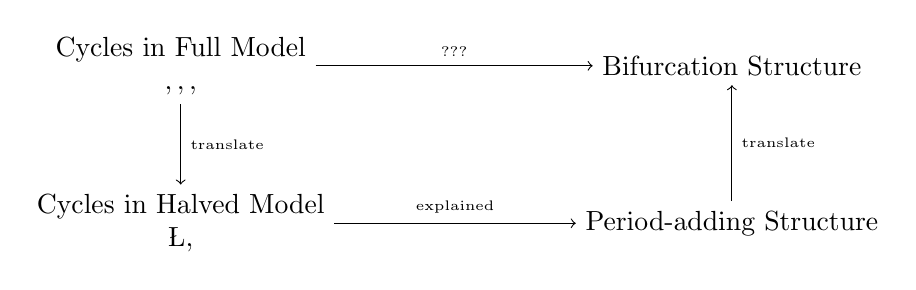
\begin{tikzpicture}[every text node part/.style={align=center}]
			\node (FC) at (0, 2) {Cycles in Full Model \\ $\A, \B, \C, \D$};
			\node (FB) at (7, 2) {Bifurcation Structure};

			\node (HC) at (0, 0) {Cycles in Halved Model \\ $\L, \R$};
			\node (HA) at (7, 0) {Period-adding Structure};

			\draw[->] (FC) -- (HC) node[midway,right] {\tiny translate};
			\draw[->] (HC) -- (HA) node[midway,above] {\tiny explained};
			\draw[->] (HA) -- (FB) node[midway,right] {\tiny translate};
			\draw[->] (FC) -- (FB) node[midway,above] {\tiny ???};
		\end{tikzpicture}
	\end{center}

	\begin{itemize}
		\item Algorithms for translating cycles between both models
		\item Formal description of novel bifurcation structure
		      \begin{itemize}
			      \item When do cycles coexist?
			      \item Symbolic Sequences
			      \item Periods
			      \item Rotation Numbers (here tuples)
		      \end{itemize}
	\end{itemize}
\end{frame}

\begin{frame}{Translation Type A (Symmetric Cycle)}
	\centering
	\begin{tikzpicture}[thick,scale=1, every node/.style={font=\huge}]
		\path[draw=none] (0,0) -- (12,2);
		%
		\coordinate (a) at (6, 0);
		\coordinate (b) at (6, -2);
		%
		% A1B2C1D2 -> L1R2
		%
		\only<1-4>{
			\node (cycleA) at (a) {$\A^{1}\B^{2}\C^{1}\D^{2}$};
		}
		\only<2>{
			\draw [decorate,decoration={brace,mirror}] (4.3, -0.8) -- (7.7, -0.8);
			\node at (6, -1.5) {4-Syllable};
		}
		\only<3>{
			\node (cycleB) at (b) {$\L^{1}\R^{2}\L^{1}\R^{2}$};
		}
		\only<4>{
			\node (cycleB) at (b) {$\L^{1}\R^{2}$};
		}
		\only<3-4>{
			\draw[->] (cycleA) -- (cycleB) node[midway,right=0.5em,scale=0.5] {$T^{-1}$};
		}
		%
		% L1R2
		%
		\only<5-8>{
			\node (cycleA) at (a) {$\L^{1}\R^{2}$};
		}
		\only<6>{
			\draw [decorate,decoration={brace,mirror}] (5.0, -0.8) -- (7.0, -0.8);
			\node at (6, -1.5) {2-Syllable};
		}
		\only<7-8>{
			\node (cycleB) at (b) {$\A^{1}\B^{2}$};
		}
		\only<8>{
			\node at (8, -2) {???};
		}
		\only<9>{
			\node (cycleA) at (a) {$\L^{1}\R^{2}\L^{1}\R^{2}$};
			\node (cycleB) at (b) {$\A^{1}\B^{2}\C^{3}\D^{4}$};
		}
		\only<7-9>{
			\draw[->] (cycleA) -- (cycleB) node[midway,right=0.5em,scale=0.5] {$T$};
		}
		%
	\end{tikzpicture}
\end{frame}

\begin{frame}{Translation Type B (Asymmetric Cycles)}
	\centering
	\begin{tikzpicture}[thick,scale=1, every node/.style={font=\huge}]
		\path[draw=none] (0,0) -- (12,2);
		%
		\coordinate (a) at (6, 0);
		\coordinate (a_) at (6, -1.5);
		\coordinate (b) at (6, -2);
		\coordinate (c) at (6, -3.5);
		\coordinate (al) at (3, 0);
		\coordinate (ar) at (9, 0);
		\coordinate (bl) at (3, -2);
		\coordinate (br) at (9, -2);
		%
		% A1B2C3D4 -> L1R2L3R4
		%
		\only<1-2>{
			\node (cycleA) at (a) {$\A^{1}\B^{2}\C^{3}\D^{4}$};
		}
		\only<2>{
			\node (cycleB) at (b) {$\L^{1}\R^{2}\L^{3}\R^{4}$};
			\draw[->] (cycleA) -- (cycleB) node[midway,right=0.5em,scale=0.5] {$T^{-1}$};
		}
		%
		\only<3-7>{
			\node (cycleAL) at (al) {$\A^{1}\B^{2}\C^{3}\D^{4}$};
			\node (cycleBL) at (bl) {$\L^{1}\R^{2}\L^{3}\R^{4}$};
			\node (cycleAR) at (ar) {$\A^{3}\B^{4}\C^{1}\D^{2}$};
		}
		\only<3-6>{
			\draw[->] (cycleAL) -- (cycleBL) node[midway,right=0.5em,scale=0.5] {$T^{-1}$};
		}
		\only<4-7>{
			\node (cycleBR) at (br) {$\L^{3}\R^{4}\L^{1}\R^{2}$};
		}
		\only<4-6>{
			\draw[->] (cycleAR) -- (cycleBR) node[midway,right=0.5em,scale=0.5] {$T^{-1}$};
		}
		\only<5>{
			\draw[->] (cycleBL) -- (cycleBR) node[midway,above=0.2em,scale=0.5] {$s_{2}$};
		}
		\only<6-7>{
			\draw[double equal sign distance] (cycleBL) -- (cycleBR) node[midway,above=0.2em,scale=0.5] {$\equiv_{2}$};
		}
		\only<7>{
			\draw[->] (cycleBR) -- (cycleAR) node[midway,right=0.5em,scale=0.5] {$T$};
			\draw[->] (cycleBL) -- (cycleAL) node[midway,right=0.5em,scale=0.5] {$T$};
		}
		%
	\end{tikzpicture}
\end{frame}


\begin{frame}{Coexistence of Cycles}
	\begin{itemize}
		\item Oddly enough, coexistence more natural
		\item Odd number of rotations (in halved model) $\Rightarrow$ No coexistence (in full model)
		      \vspace{1em}
		\item Child of two nodes with coexistence has no coexistence
		\item Child of two nodes with no coexistence has no coexistence
		\item Child of a node with and a node with no coexistence has coexistence
	\end{itemize}

\end{frame}

%%% Local Variables:
%%% mode: latex
%%% TeX-master: "../Vortrag_Frauenhofer_Weik"
%%% End:


\sectionframe{Current Development}
\section{Current}

\begin{frame}{Model in Continuous Time}
	\vspace{-1em}
	\begin{columns}
		\begin{column}{.3 \textwidth}
			\begin{align*}
				\overset{\cdot}{x} & = \lambda (x - 1) \quad & \text{if } & K_{F} = +1 \\
				\overset{\cdot}{x} & = \lambda x       \quad & \text{if } & K_{F} = 0  \\
				\overset{\cdot}{x} & = \lambda (x + 1) \quad & \text{if } & K_{F} = -1
			\end{align*}

			Switching at
			\begin{align*}
				V_{ref} \pm \chi_{c} \\
				V_{ref} \pm \chi_{0}
			\end{align*}
		\end{column}
		\begin{column}{.7 \textwidth}
			\begin{figure}
				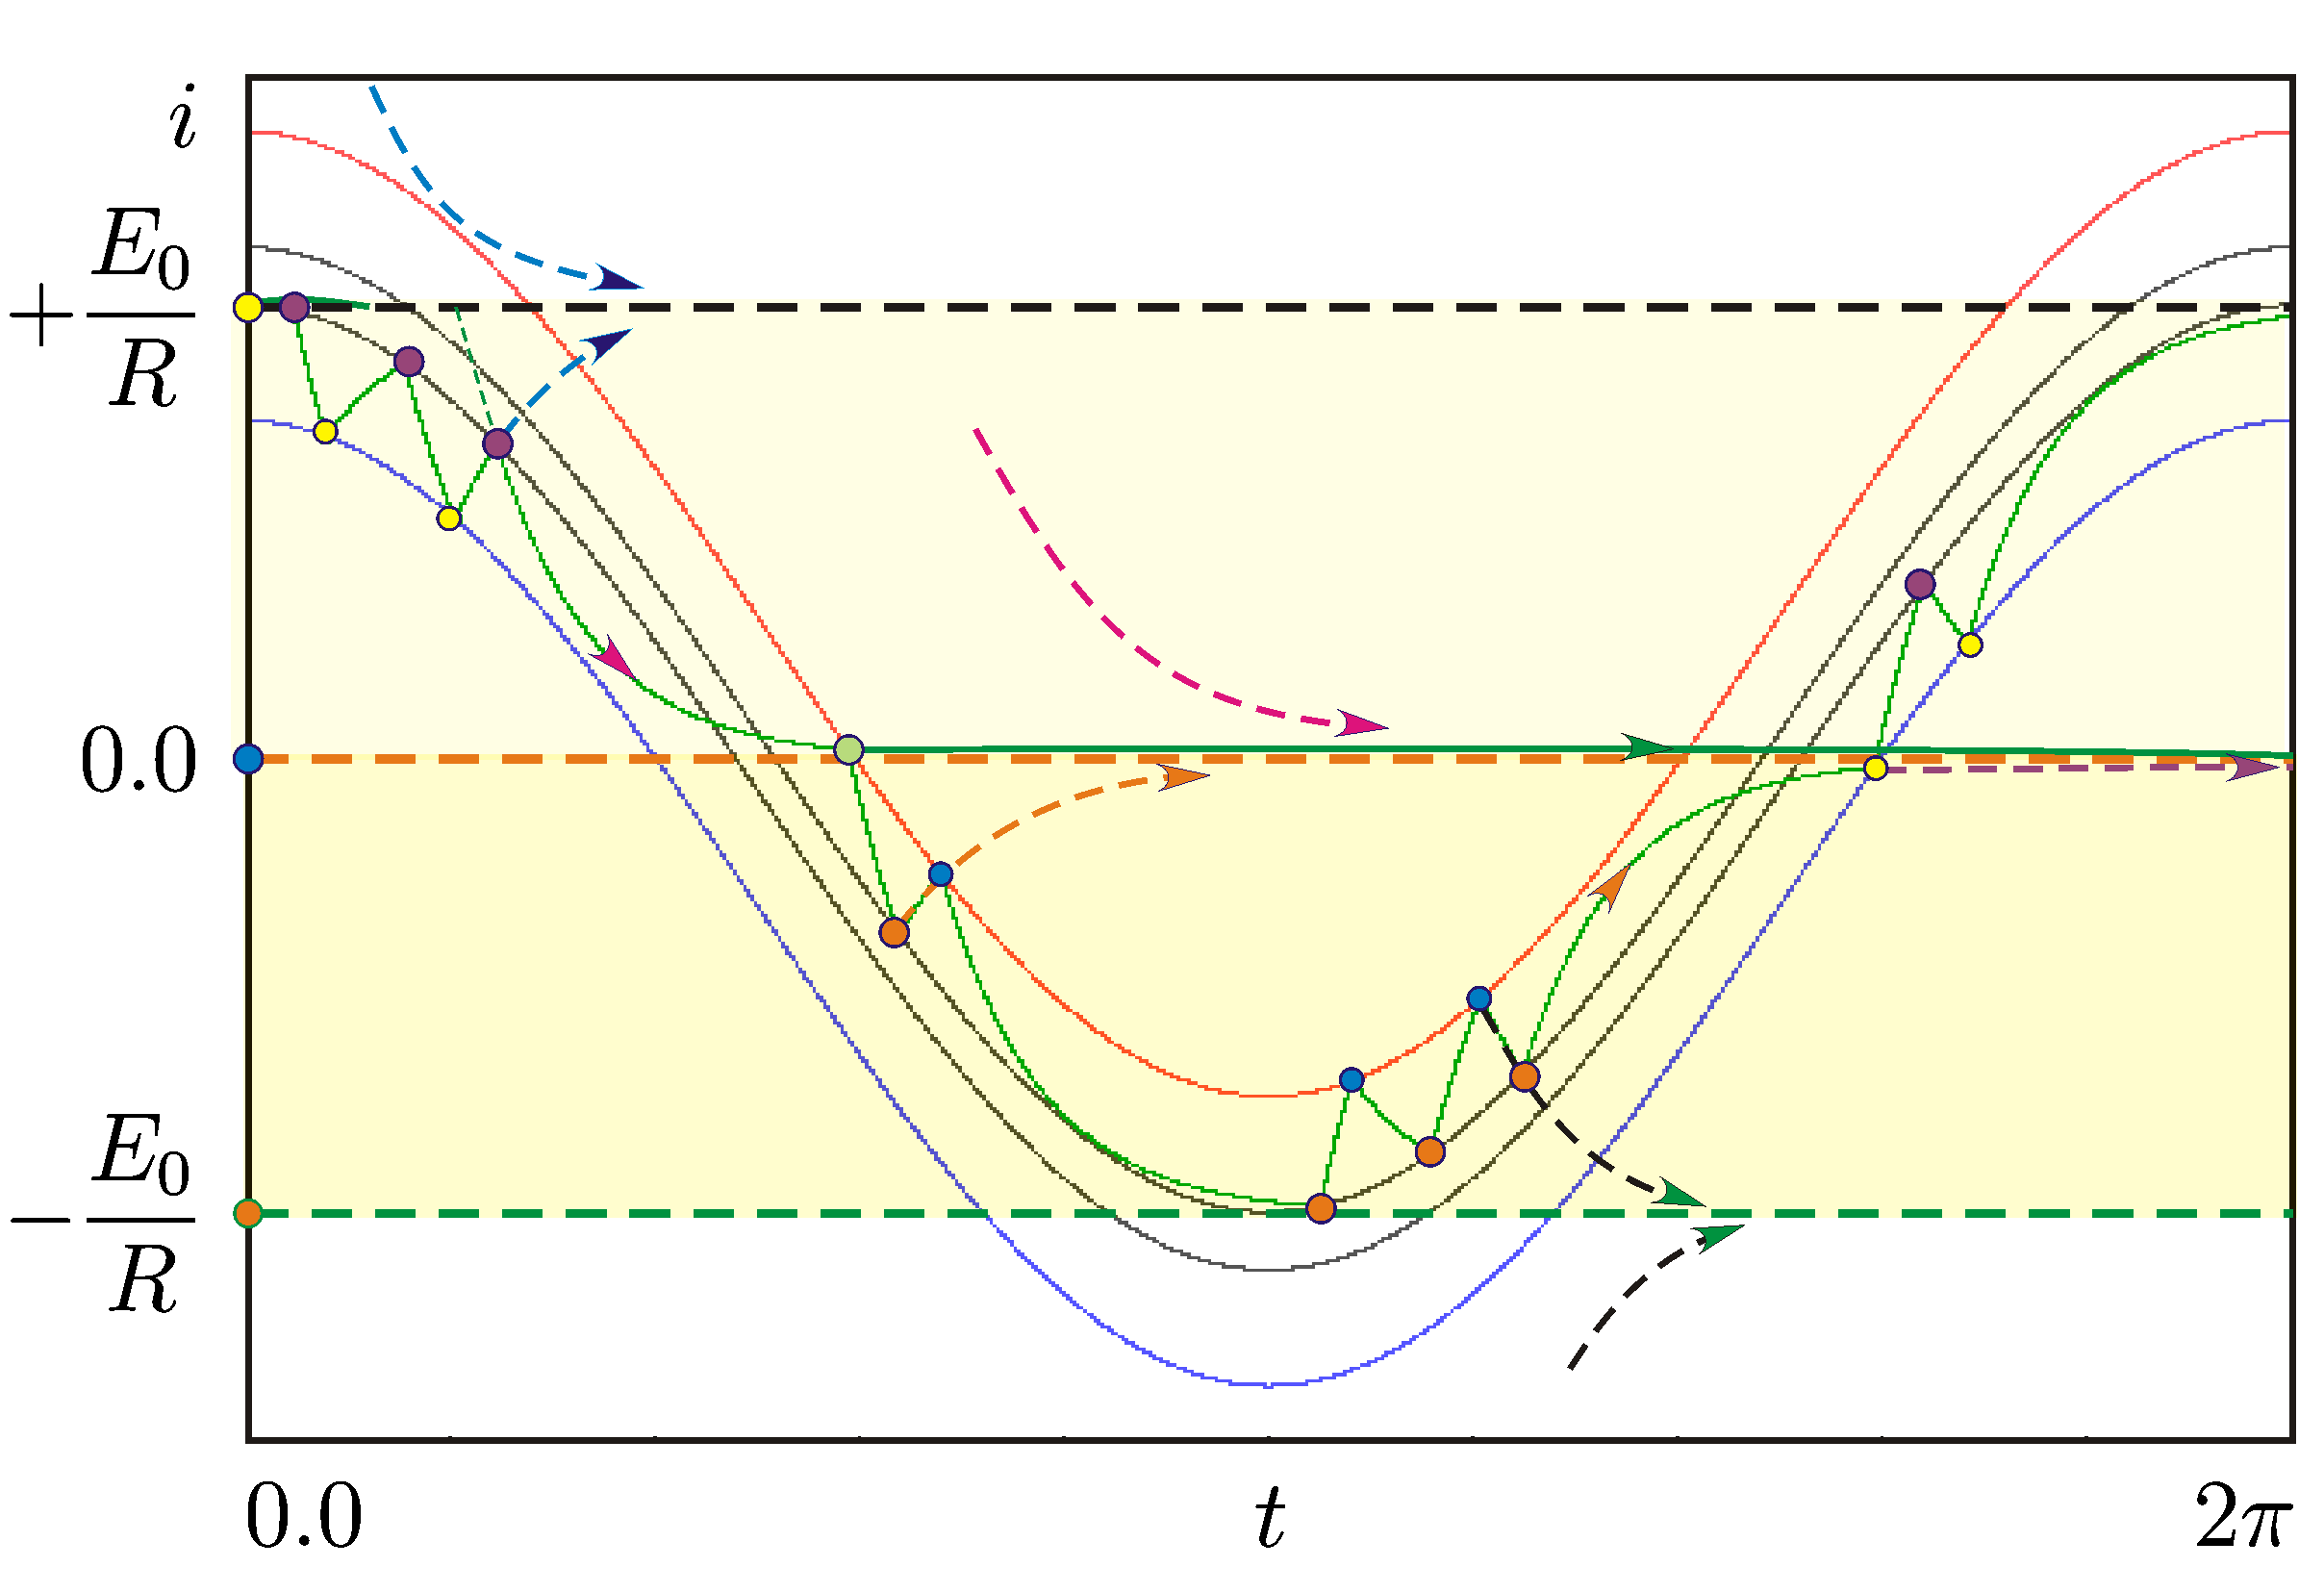
\includegraphics[width=0.7 \textwidth]{Figs/continuous_model.png}
			\end{figure}

			\flushright{[Zhusubaliyev]}
		\end{column}
	\end{columns}
\end{frame}

\begin{frame}{Model in Concrete Time}
	\vspace{-1em}
	\begin{columns}
		\begin{column}{.6 \textwidth}
			\begin{align*}
				(q \cos(\tau) - \chi_{c}) \cdot e^{z^{+}}                      = q \cos(\tau + z^{+}) - \chi_{0}            \\
				(q \cos(\tau + z^{+}) - \chi_{0} - 1) \cdot e^{z_{1}^{+}}      + 1  =                                \qquad \\
				q \cos(\tau + z^{+} + z_{1}^{+}) - \chi_{c}                                                                 \\\\
				(q \cos(\tau) - \chi_{c}) \cdot e^{z_{0}^{+}}                  = q \cos(\tau + z_{0}^{+}) + \chi_{0}        \\
				(q \cos(\tau + z_{0}^{+}) + \chi_{0} + 1) \cdot e^{z_{2}^{+}}  - 1  =                               \qquad  \\
				\hfill q \cos(\tau + z^{+} + z_{2}^{+}) + \chi_{c}
			\end{align*}
		\end{column}
		\begin{column}{.4 \textwidth}
			\begin{figure}
				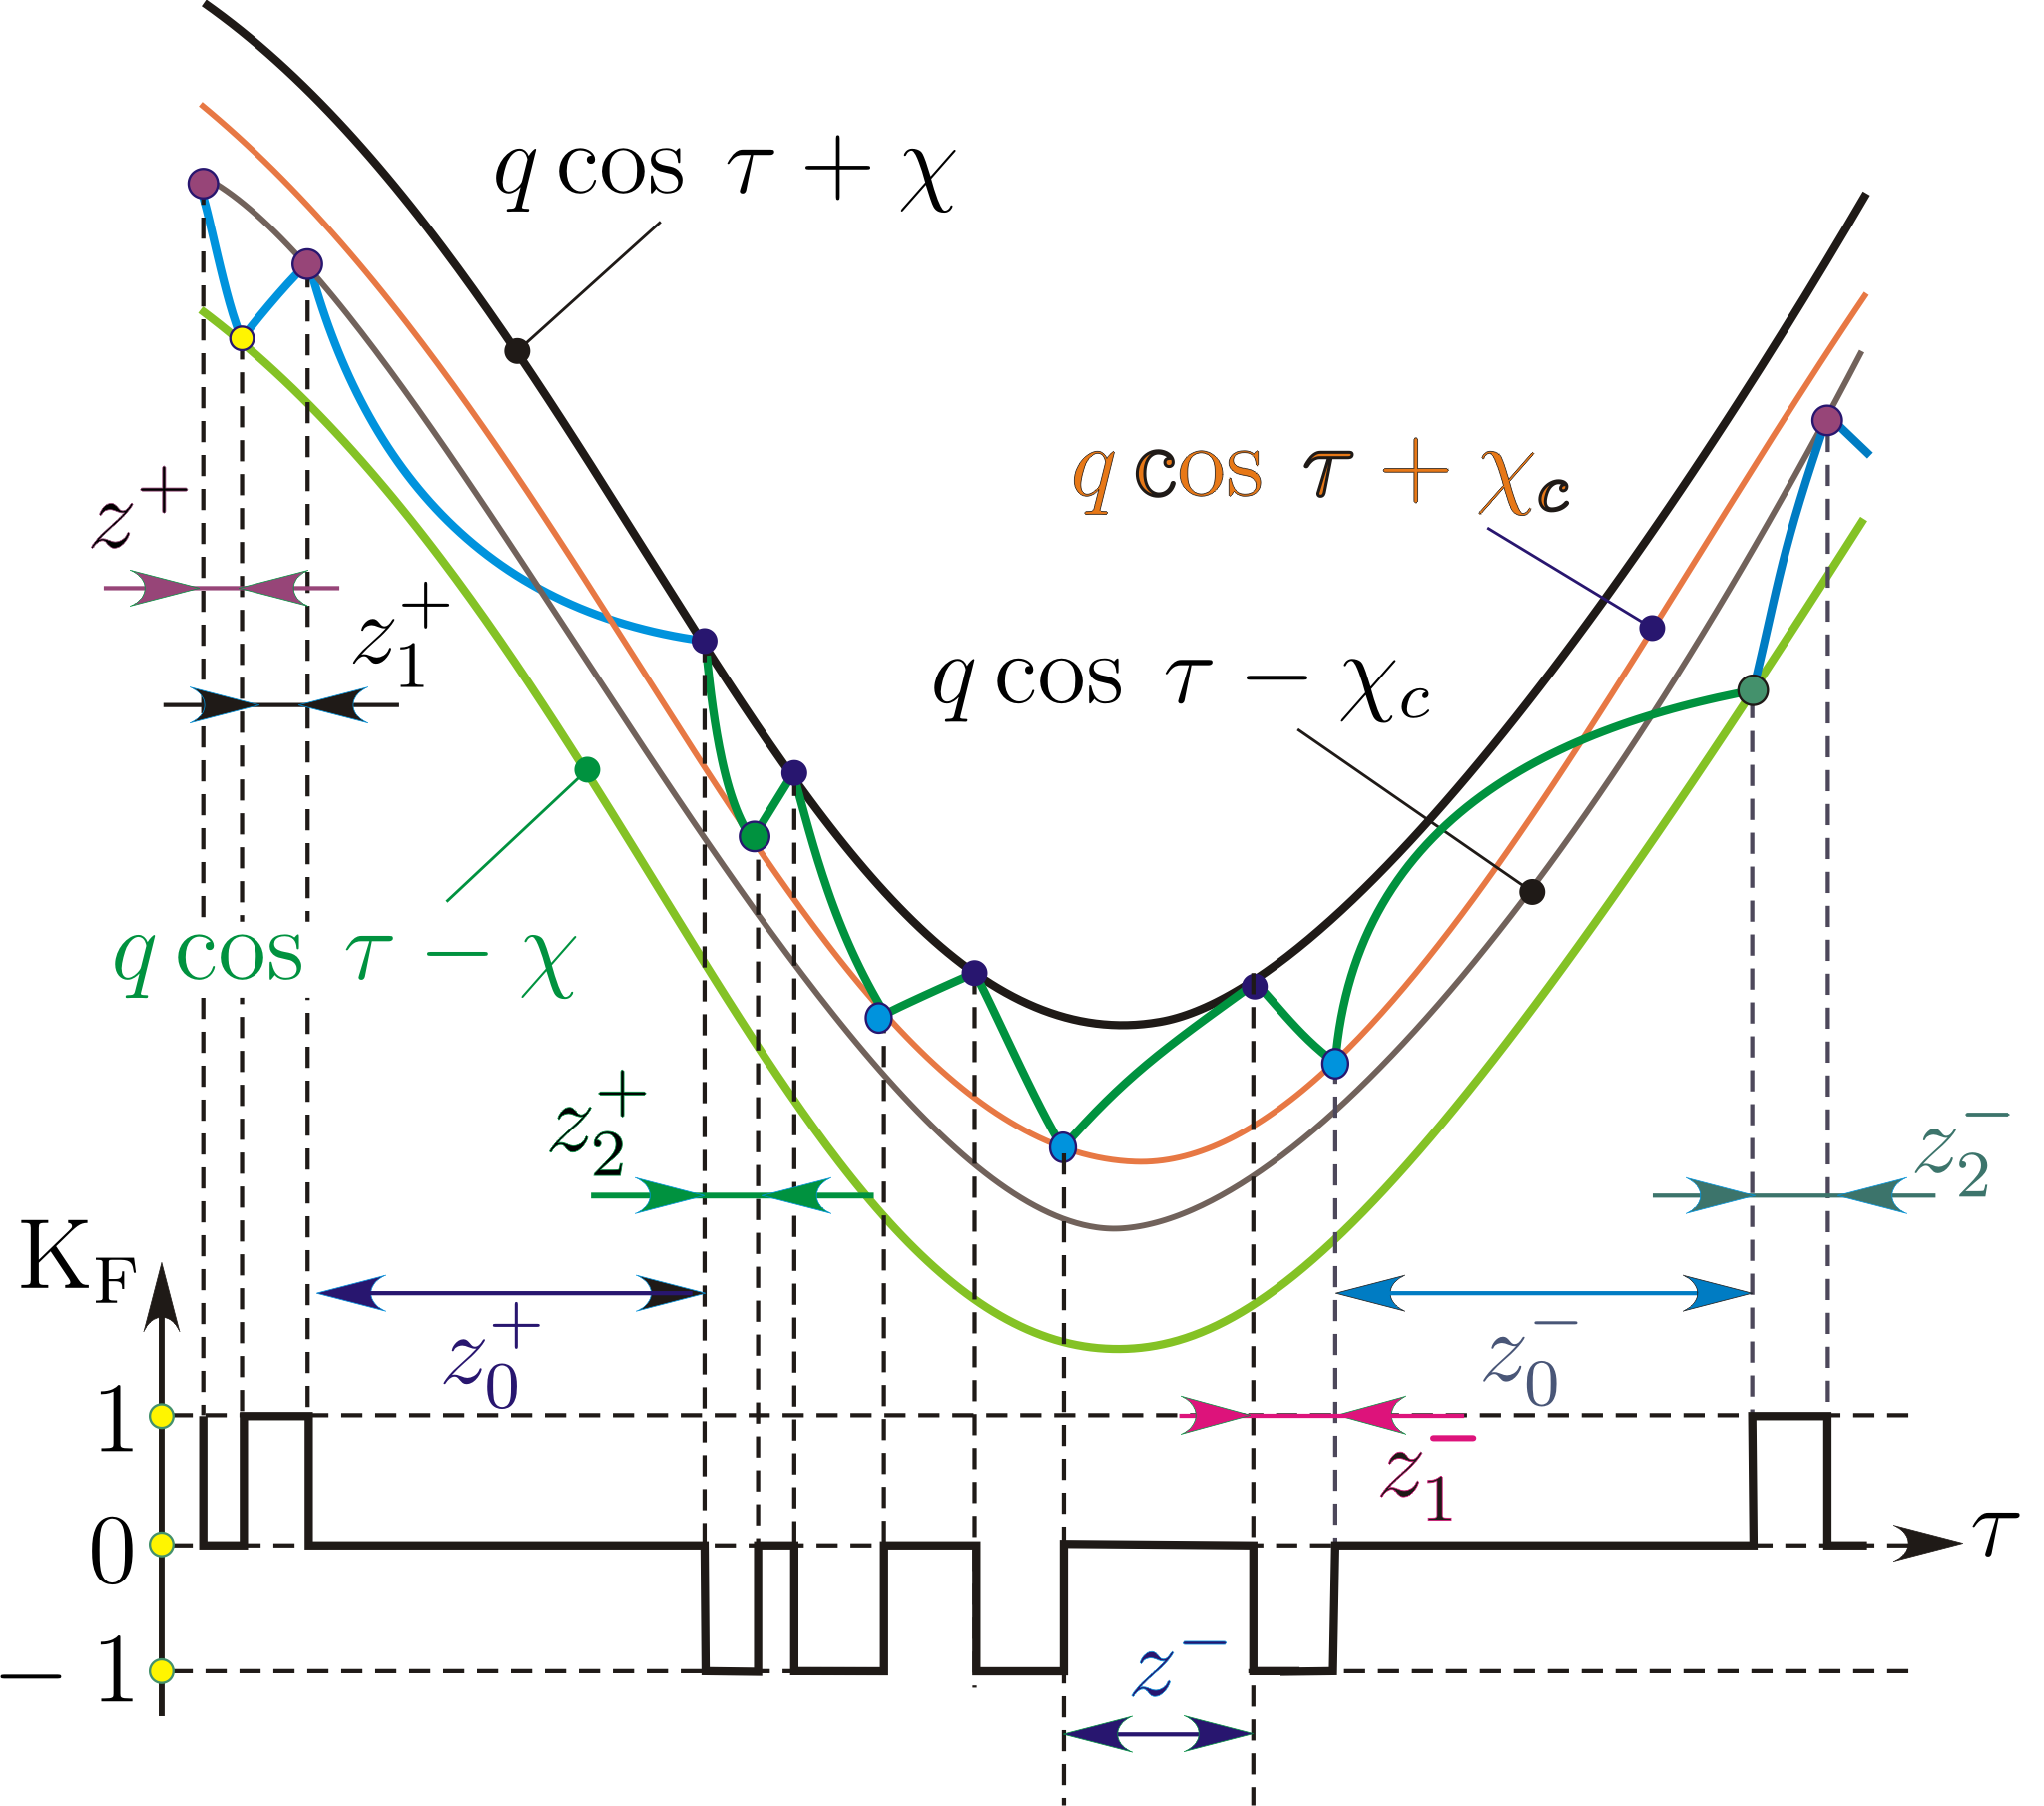
\includegraphics[width=0.9 \textwidth]{Figs/discrete_model_derivation.png}
			\end{figure}
		\end{column}
	\end{columns}

	\flushright{[Avrutin]}
\end{frame}

\begin{frame}{Model in Concrete Time}
	\vspace{-1em}
	\begin{columns}
		\begin{column}{.5 \textwidth}
			\begin{align*}
				\tau \mapsto  \tau + \begin{cases}
					                     z^{+} + z_{1}^{+}     & \text{if } z^{+} \leq z_{0}^{+} \\
					                     z_{0}^{+} + z_{2}^{+} & \text{if } z^{+} > z_{0}^{+}
				                     \end{cases}
			\end{align*}
			\vspace{1em}

			Repeat the whole process to get
			\begin{align*}
				z^{-}, z_{1}^{-}, z_{0}^{-}, \text{ and } z_{2}^{-}
			\end{align*}
		\end{column}
		\begin{column}{.5 \textwidth}
			\begin{figure}
				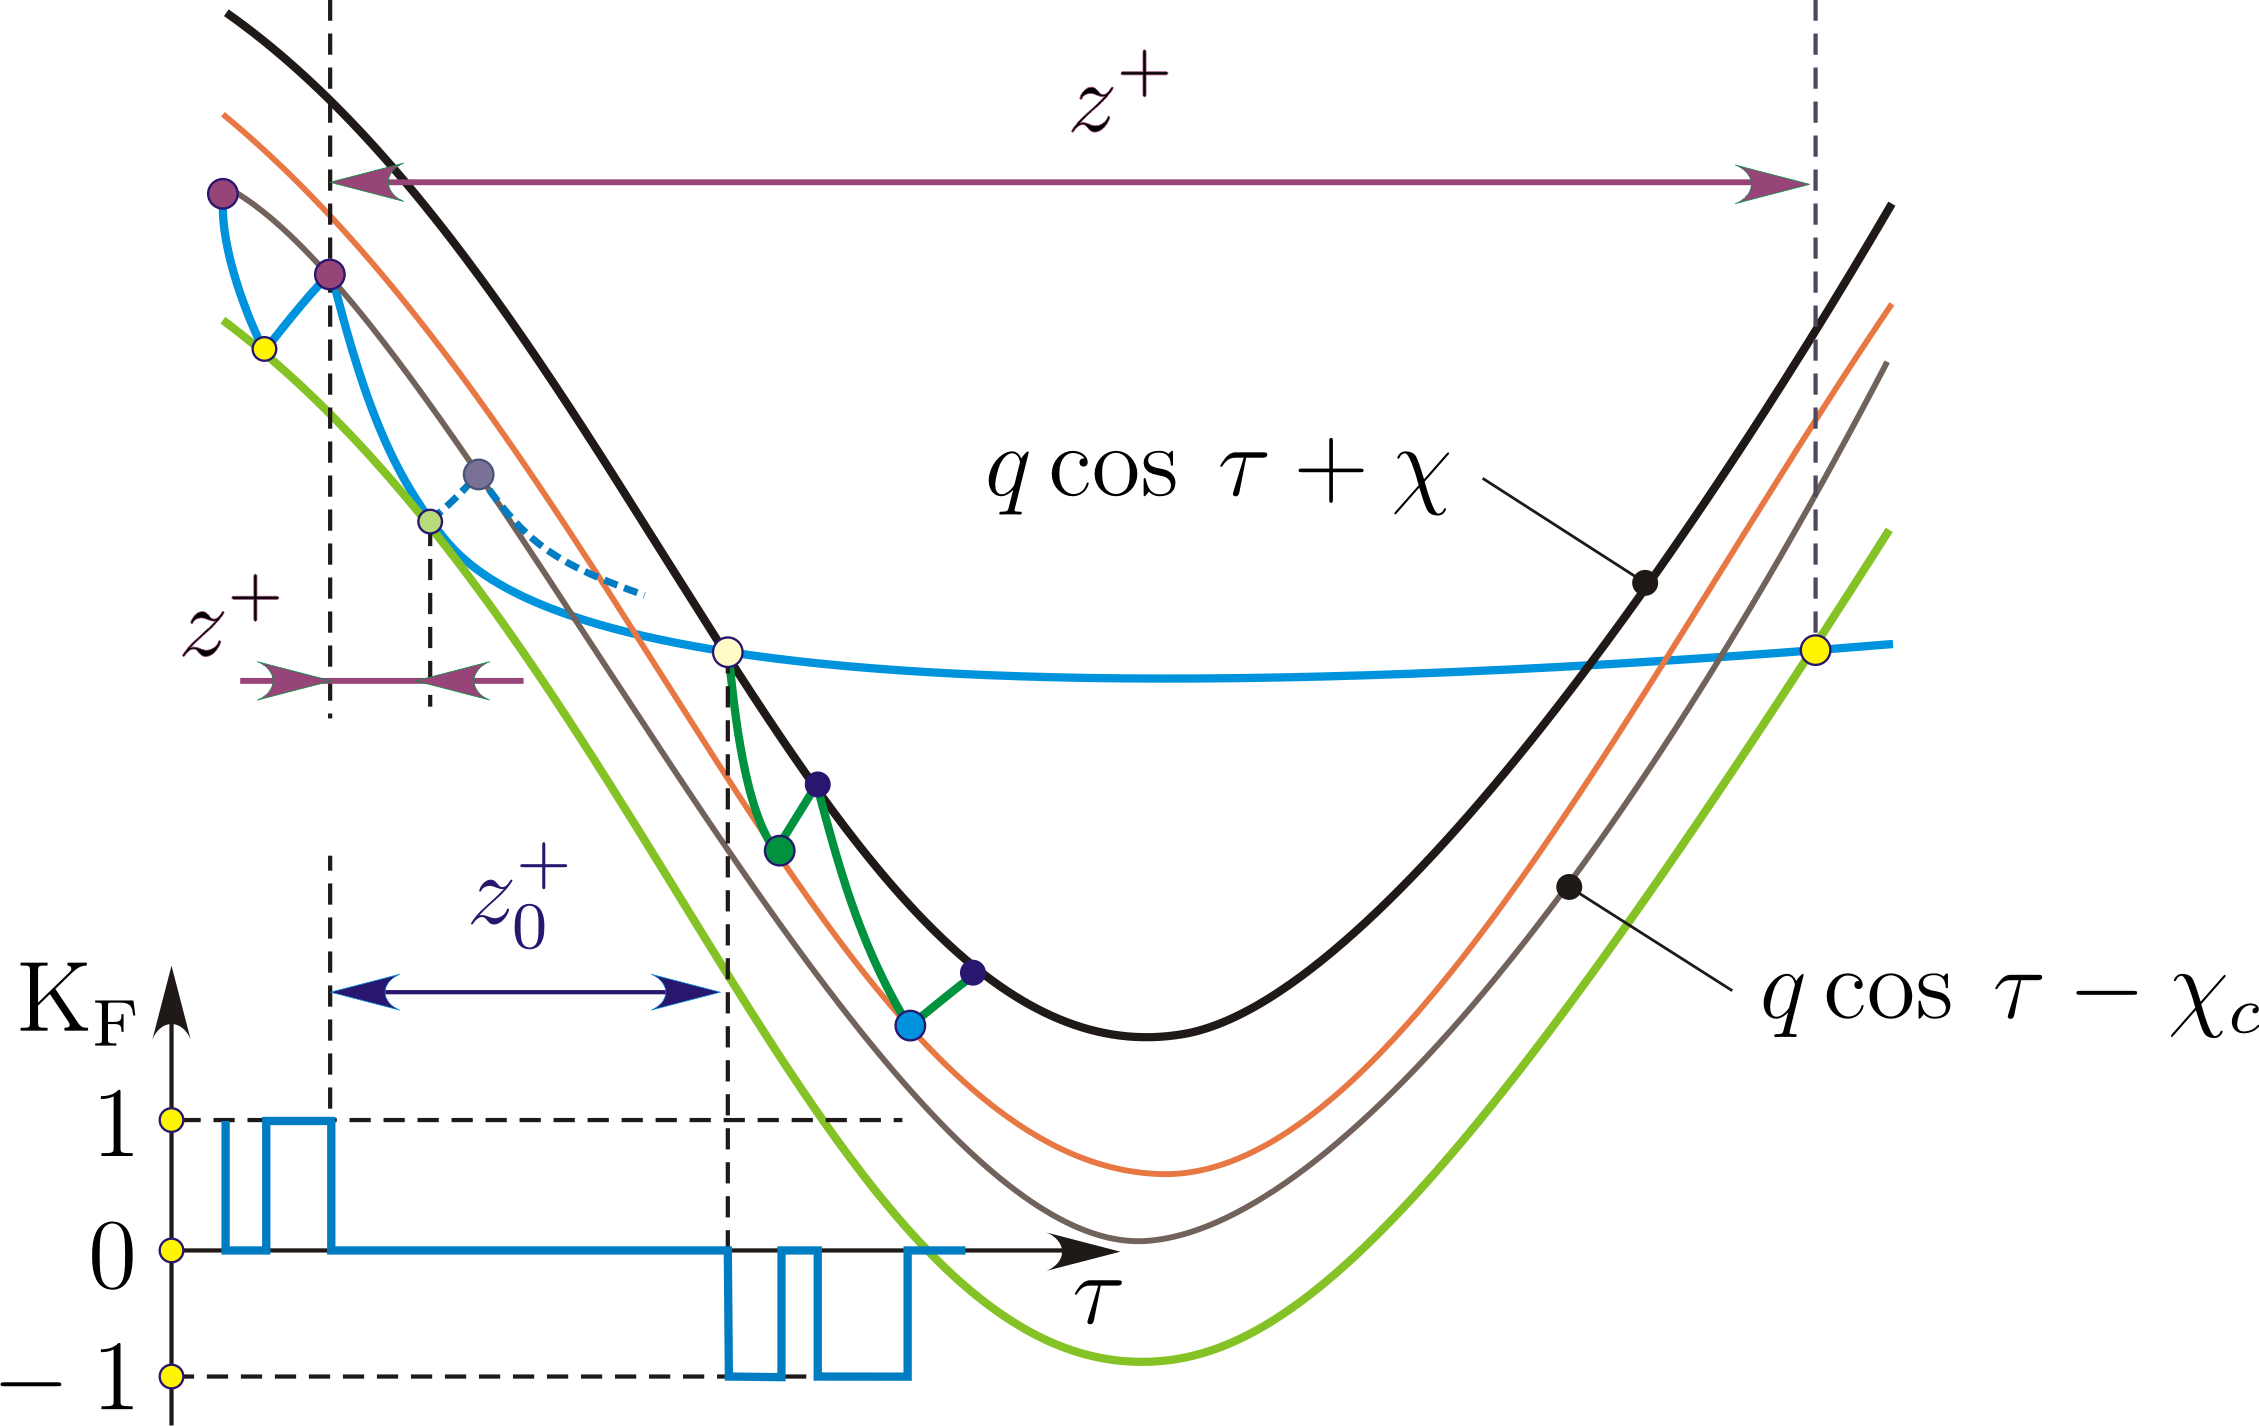
\includegraphics[width=1 \textwidth]{Figs/discrete_model_derivation_cases.png}
			\end{figure}
		\end{column}
	\end{columns}

	\flushright{[Avrutin]}
\end{frame}

%\sectionframe{Original Model}
\section{OG}

\begin{frame}{Model Origin}
	\begin{itemize}
		\item DC/AC power converter with hysteresis control
		\item The converter switches $\Rightarrow$ model is piecewise-smooth
		\item The converter has hysteresis control $\Rightarrow$ model is also discontinuous
		      \pause \vspace{1em}
		\item We focus on the time-discrete model
		\item It maps phase of the last switch $\theta_n$ to the phase of the next switch $\theta_{n+1}$
	\end{itemize}
\end{frame}

\begin{frame}{Model Definition (1/2)}
	\vspace{-2.0em}
	\begin{align*}
		\theta_{n+1} & =  F(\theta_n) \mod 2 \pi
		\\
		F(\theta)    & = \begin{cases}
			                 F_1(\theta) & \text{if } q \cdot \cos(\theta) > 0 \\
			                 F_2(\theta) & \text{if } q \cdot \cos(\theta) < 0
		                 \end{cases}
		\\
		F_1(\theta)  & = \begin{cases}
			                 \theta + z_{L_+} + z_1 & \text{if } z_{L_+} < z_{L_0} \\
			                 \theta + z_{L_0} + z_2 & \text{if } z_{L_+} > z_{L_0}
		                 \end{cases}
		\\
		F_2(\theta)  & = \begin{cases}
			                 \theta + z_{R_+} + z_3 & \text{if } z_{R_+} < z_{R_0} \\
			                 \theta + z_{R_0} + z_4 & \text{if } z_{R_+} > z_{R_0}
		                 \end{cases}
	\end{align*}

	\pause
	\vspace{2em}
	This looks ok, but how are these values defined?
	\begin{align*}
		z_1, z_2, z_3, z_4, z_{L_+}, z_{L_-}, z_{R_+}, \text{ and } z_{R_0}
	\end{align*}
\end{frame}

\begin{frame}{Model Definition (2/2)}
	\vspace{-1em}
	The smallest non-negative solutions to the following implicit equations
	\begin{subequations}
		\begin{align*}
			(q \cdot \cos(\theta) + \mu \cdot \chi) \cdot e^{\lambda \cdot z_{L_+}}
			 & = q \cdot \cos(\theta + z_{L_+}) + \chi                  \\
			(q \cdot \cos(\theta) + \mu \cdot \chi) \cdot e^{\lambda \cdot z_{L_0}}
			 & = q \cdot \cos(\theta + z_{L_0}) - \chi                  \\
			(q \cdot \cos(\theta) - \mu \cdot \chi) \cdot e^{\lambda \cdot z_{R_+}}
			 & = q \cdot \cos(\theta + z_{R_+}) - \chi                  \\
			(q \cdot \cos(\theta) - \mu \cdot \chi) \cdot e^{\lambda \cdot z_{R_0}}
			 & = q \cdot \cos(\theta + z_{R_0}) + \chi
			\\
			(q \cdot \cos(\theta + z_{L_+}) + \chi + 1) \cdot e^{\lambda \cdot z_1} - 1
			 & = q \cdot  \cos(\theta + z_{L_+} + z_1) + \mu \cdot \chi \\
			(q \cdot \cos(\theta + z_{L_0} + z_2) - \chi - 1) \cdot e^{\lambda \cdot z_2} + 1
			 & = q \cdot  \cos(\theta + z_{L_0} + z_2) - \mu \cdot \chi \\
			(q \cdot \cos(\theta + z_{R_+}) + \chi + 1) \cdot e^{\lambda \cdot z_3} - 1
			 & = q \cdot  \cos(\theta + z_{L_+} + z_1) + \mu \cdot \chi \\
			(q \cdot \cos(\theta + z_{R_0} + z_4) - \chi - 1) \cdot e^{\lambda \cdot z_4} + 1
			 & = q \cdot  \cos(\theta + z_{R_0} + z_2) - \mu \cdot \chi
		\end{align*}
	\end{subequations}
	\begin{flushright}
		Definition from \cite{akyuz2022}
	\end{flushright}
\end{frame}

\begin{frame}{Unusual Bifurcation Structure}
	\begin{figure}
		\only<1>{
			\includegraphics[width=0.45 \textwidth]{../Figures/2/2.3/result.png}
		}
		\only<2>{
			\stackunder[5pt]{
				\includegraphics[width=0.3 \textwidth]{../Figures/2/2.4a/result.png}
			}{$A:\:\A^3\B^3\C^3\D^3$}
			\stackunder[5pt]{
				\includegraphics[width=0.3 \textwidth]{../Figures/2/2.4b/result.png}
			}{$B:\:\A^3\B^3\C^2\D^4,\:\A^2\B^4\C^3\D^3$}
			\stackunder[5pt]{
				\includegraphics[width=0.3 \textwidth]{../Figures/2/2.4c/result.png}
			}{$C:\:\A^2\B^4\C^2\D^4$}
		}
	\end{figure}
	\pause
	\vspace{1em}
	Symmetry $F(\theta + \pi) = F(\theta) + \pi \mod 2\pi$ \hfill \cite{akyuz2022}
\end{frame}

%\sectionframe{Archetypal Model}
\section{Archetypal}

\begin{frame}{Approach}
	\vspace{-1em}
	Construct an archetypal model with similar characteristics
	\pause
	\begin{itemize}
		\item Symmetry $F(\theta + \pi) = F(\theta) + \pi \mod 2\pi$ \hfill \cite{akyuz2022} \pause
		\item Model branches $f_\A$ and $f_\C$ quadratic
		\item Model branches $f_\B$ and $f_\D$ simplified as linear \pause
		\item $E_0$: The values at the left border of branches $F_{\B}$ and $F_{\D}$ move down
		\item $\chi_0$: Branches $F_{\A}$ and $F_{\C}$ move up
	\end{itemize}

	\begin{figure}
		\stackunder[5pt]{
			\includegraphics[width=0.2 \textwidth]{../Figures/5/5.4a/illustration.png}
		}{Effect of $E_0$}
		\stackunder[5pt]{
			\includegraphics[width=0.2 \textwidth]{../Figures/5/5.4b/illustration.png}
		}{Effect of $\chi_0$}
		\only<3->{
			\stackunder[5pt]{
				\includegraphics[width=0.2 \textwidth]{../Figures/5/5.13a/illustration.png}
			}{Effect of $\alpha$}
			\stackunder[5pt]{
				\includegraphics[width=0.2 \textwidth]{../Figures/5/5.13b/illustration.png}
			}{Effect of $\beta$}
		}
	\end{figure}
\end{frame}

\begin{frame}{Archetypal Model Dynamics}
	\only<1>{
		\begin{figure}
			\stackunder[5pt]{
				\includegraphics[width=0.3 \textwidth]{99_Yunus/2D_Period_Zoomed/result.png}
			}{Original model}
			\qquad
			\stackunder[5pt]{
				\includegraphics[width=0.3 \textwidth]{../Figures/6/6.1a/result.png}
			}{Archetypal model}
		\end{figure}
	}
	\only<2>{
		\begin{columns}
			\begin{column}{.9 \textwidth}
				\begin{figure}
					\centering
					\stackunder[5pt]{
						\includegraphics[height=0.45\textheight]{../Figures/6/6.2c/result.png}
					}{$C_{16}:\:\Cycle{\A^6\B^2\C^6\D^2}$}
					\stackunder[5pt]{
						\includegraphics[height=0.45\textheight]{../Figures/6/6.2d/result.png}
					}{$D_{16}:\:\Cycle{\A^6\B^2\C^5\D^3},\Cycle{\A^5\B^3\C^6\D^2}$}
					\stackunder[5pt]{
						\includegraphics[height=0.45\textheight]{../Figures/6/6.2e/result.png}
					}{$E_{16}:\:\Cycle{\A^5\B^3\C^5\D^3}$}
				\end{figure}
			\end{column}
			\begin{column}{.2 \textwidth}
				\vspace{-4em}
				\begin{center}
					\hspace{-2em}
					\includegraphics[height=0.3 \textheight]{../Figures/6/6.1a/result.png}
				\end{center}
			\end{column}
		\end{columns}
	}
\end{frame}

\begin{frame}{Definition of the Archetypal Model (1/2)}
	\vspace{-1.0em}
	\begin{align*}
		x_{n+1} = f(x_n) \mod 1
	\end{align*}
	\begin{align*}
		f(x) & = \begin{cases}
			         g(x)                                        & \text{ if } x < \frac{1}{2} \\
			         g\left(x - \frac{1}{2}\right) + \frac{1}{2} & \text{ else}
		         \end{cases}
	\end{align*}
	\begin{align*}
		g(x) & = \begin{cases}
			         g_L(x) = a_L \cdot x^2 + b_L \cdot x + c_L & \text{ if } x < \frac{1}{4} \\
			         g_R(x) = b_R \cdot x + c_R                 & \text{ else}
		         \end{cases}
	\end{align*}
\end{frame}

\begin{frame}{Definition of the Archetypal Model (2/2)}
	\vspace{-1em}
	\begin{columns}
		\begin{column}{.7 \textwidth}
			Fixed parameters:
			\begin{align*}
				a_L = 4 \text{ and } b_L = -\tfrac{1}{2}
			\end{align*}
			Variable parameters
			\begin{align*}
				 & c_L, b_R, c_R                                                                                                              \\
				\text{where} \qquad
				 & c_L = \beta,                                                                                                               \\
				 & b_R = -4 \cdot g_R\left(\tfrac{1}{4}\right) + 4 \cdot g_R\left(\tfrac{1}{2}\right),                                        \\
				 & c_R = 2 \cdot g_R\left(\tfrac{1}{4}\right) - 1 \cdot g_R\left(\tfrac{1}{2}\right),                                         \\[1em]
				\text{and} \qquad
				 & g_R\left(\tfrac{1}{4}\right) = \alpha, \text{and } g_R\left(\tfrac{1}{2}\right) = \tfrac{1}{2} + \epsilon \text{ is fixed}
			\end{align*}
		\end{column}
		\begin{column}{.3 \textwidth}
			\begin{figure}
				\centering
				\includegraphics[height=.5 \textheight]{60_MinimalRepr/ParameterEffects/AB/illustration.png}
				%\caption*{Illustration of the parameters $A$ and $B$}
			\end{figure}
		\end{column}
	\end{columns}
\end{frame}

\begin{frame}{Bifurcation Analysis}
	\begin{columns}
		\begin{column}{.5 \textwidth}
			\only<1>{
				At the boundaries of the ``type B'' parameter region with the cycles $\Cycle{\A^5\B^3\C^4\D^4}$ and $\Cycle{\A^4\B^4\C^5\D^3}$
			}
			\only<2->{
				\begin{itemize}
					\item Only border collision bifurcations
					\item Symmetry $\Rightarrow$ All collisions double
					\item At border at $x$ and $x + \frac{1}{2} \mod 1$
				\end{itemize}
				\vspace{1em}
				\begin{itemize}
					\item ``Type A'': cycle collides with two borders at once (unusual)
					\item ``Type B'': each of the coexisting cycles collides with one border
				\end{itemize}
			}
		\end{column}
		\begin{column}{.5 \textwidth}
			\vspace{-3em}
			\begin{figure}
				\centering
				\only<1>{
					\subfloat{ \includegraphics[height=.7 \textheight]{../Figures/6/6.3b/result.png} }
				}
				\only<2->{
					\vspace{-2.5em}
					\subfloat{ \includegraphics[height=.2 \textheight]{../Figures/6/6.3b/result.png} }
				}
				\only<2>{
					\begin{minipage}{.4 \textwidth}
						\centering
						\vspace{-3em}
						$F_{16}^\uparrow$
					\end{minipage}
					\\
					\subfloat{\includegraphics[height=.7 \textheight]{../Figures/6/6.4/result.png}}
				}
				\only<3>{
					\begin{minipage}{.4 \textwidth}
						\centering
						\vspace{-3em}
						$F_{16}^\downarrow$
					\end{minipage}
					\\
					\subfloat{\includegraphics[height=.7 \textheight]{../Figures/6/6.5/result.png}}
				}
				\only<4>{
					\begin{minipage}{.4 \textwidth}
						\centering
						\vspace{-3em}
						$F_{16}^\leftarrow$
					\end{minipage}
					\\
					\subfloat{\includegraphics[height=.7 \textheight]{../Figures/6/6.6/result.png}}
				}
				\only<5>{
					\begin{minipage}{.4 \textwidth}
						\centering
						\vspace{-3em}
						$F_{16}^\rightarrow$
					\end{minipage}
					\\
					\subfloat{\includegraphics[height=.7 \textheight]{../Figures/6/6.7/result.png}}
				}
			\end{figure}
		\end{column}
	\end{columns}
\end{frame}

\begin{frame}{Overlapping Parameter Regions}
	\vspace{-1em}
	\begin{columns}
		\begin{column}{.5 \textwidth}
			Coexistence scenarios:
			\begin{itemize}
				%\item 1: ``Type A'' ($L$)
				\item 2: Two different ``Type A'' \\ ($M, N, O,$ and $P$)
				      %\item 2: ``Type B'' pair ($Q$)
				\item 3: ``Type B'' pair and ``Type A'' \\ ($R, S, T,$ and $U$)
				\item 4: ``Type B'' pair \\ and two different ``Type A'' \\ ($V, W, X,$ and $Y$)
			\end{itemize}

			\vspace{.5em}
			The coexistence of 4 cycles was overlooked in the original model!
		\end{column}
		\begin{column}{.5 \textwidth}
			\vspace{-5em}
			\begin{figure}
				\centering
				\only<1>{
					\vspace{-.5em}
					\subfloat{ \includegraphics[height=0.5 \textheight]{../Figures/6/6.8a/result.png} }
					\\[.1em]
					\hspace{1em}
					\subfloat{ \includegraphics[height=0.5 \textheight]{../Figures/6/6.8b/result.png} }
				}
				\only<2->{
					\subfloat{ \includegraphics[height=0.2 \textheight]{60_MinimalRepr/2D_Regions_E/result.png} }
					\subfloat{ \includegraphics[height=0.2 \textheight]{60_MinimalRepr/2D_Regions_F/result.png} }
					\\
				}
				\only<2>{
					\stackunder[4pt]{
						\includegraphics[height=.7 \textheight]{60_MinimalRepr/Cobweb_M/Manual/result.png}
					}{At the point $M$}
				}
				\only<3>{
					\stackunder[4pt]{
						\includegraphics[height=.7 \textheight]{60_MinimalRepr/Cobweb_U/Manual/result.png}
					}{At the point $U$}
				}
				\only<4>{
					\stackunder[5pt]{
						\includegraphics[height=.7 \textheight]{60_MinimalRepr/Cobweb_X/Manual/result.png}
					}{At the point $X$}
				}
				\only<5>{
					\stackunder[4pt]{
						\includegraphics[width=.7 \textheight]{../Figures/6/6.11b/result.png}
					}{Four coexisting cycles in the original model}
				}
			\end{figure}
		\end{column}
	\end{columns}
\end{frame}

\begin{frame}{Development and Application of the Archetypal Model}
	\vspace{-1em}
	We confirmed that the archetypal map approach works
	\vspace{1em}
	\pause
	\begin{itemize}
		\item Model function shape similar to the original model
		      \begin{itemize}
			      \item Symmetry: $f\left(x + \frac{1}{2}\right) = f(x) + \frac{1}{2}$ for $x \in \left[0, \frac{1}{2}\right)$
			      \item Branches $f_\A, f_\C$ quadratic with local minima (necessary for ``type B'' cycles, proven)
			      \item Branches $f_\B, f_\D$ can be linear
		      \end{itemize}
		      \pause
		\item Parameter effects similar to the original model
		      \begin{itemize}
			      \item $\alpha$ for the values at the left borders of $f_\B$ and $f_\D$
			      \item $\beta$ for the offset of $f_\A$ and $f_\C$
		      \end{itemize}
		      \pause
		\item Description and explanation of the period-incrementing structure
		      \begin{itemize}
			      \item Chain of alternating ``type A'' and ``type B'' parameter regions with the same period
			      \item All border collision bifurcations double (because of the symmetry)
			      \item Coexistence of up to four cycles
		      \end{itemize}
	\end{itemize}
\end{frame}

%\sectionframe{Period-adding-like Structures in the Archetypal Model}
\section{Period-adding-like}

\begin{frame}{Configuration Changes}
	\vspace{-1em}
	\begin{figure}
		\includegraphics[width=.3 \textwidth]{60_MinimalRepr/Cobweb_E16/result.png}
		\quad
		\includegraphics[width=.3 \textwidth]{62_MinimalRepr_Adding/Cob_1_ZCorn/result.png}
	\end{figure}
	\vspace{1em}
	Got rid of the local minima on branches $f_\A$ and $f_\C$
\end{frame}

\begin{frame}{Period-adding-like Structures in the Archetypal Model}
	\begin{figure}
		\includegraphics[width=.4 \textwidth]{62_MinimalRepr_Adding/2D_Regions_1/Manual/result.png}
		\quad
		\includegraphics[width=.4 \textwidth]{62_MinimalRepr_Adding/2D_Period_add_zoom/result.png}
	\end{figure}
\end{frame}

%\begin{frame}{Changes to the Bifurcation Structure}
%	\begin{itemize}
%		\item ``Type B'' parameter regions disappeared
%		\item ``Type A'' parameter regions of the same chains start overlapping
%		      \pause
%		\item New space in-between chains
%	\end{itemize}
%\end{frame}

\begin{frame}{Describing the Period-adding-like Structures}
	\vspace{-1em}
	\begin{figure}
		\only<1>{
			\includegraphics[width=.4 \textwidth]{62_MinimalRepr_Adding/2D_Period_add_zoom_hor/result.png}
			\qquad
			\includegraphics[width=.4 \textwidth]{../Figures/7/7.12b/result.png}
		}
		\only<2>{
			\includegraphics[width=.7 \textwidth]{../Figures/7/7.13/adding.png}
		}
	\end{figure}
\end{frame}

\begin{frame}{Result of Describing the Structures}
	This is not period-adding
	\begin{itemize}
		\item Periods don't add
		\item Symbolic sequences don't concatenate
	\end{itemize}
	\vspace{1em}
	But it is similar
\end{frame}

%\sectionframe{The Halved Archetypal Model}
\section{Halved}

\begin{frame}{Lifting the Model}
	\vspace{-1em}
	\begin{columns}
		\begin{column}{.4 \textwidth}
			\begin{figure}
				\includegraphics[width=\textwidth]{63_MinimalRepr_Adding_Halved/Cob_Vis_s/Manual/result.png}
			\end{figure}
		\end{column}
		\begin{column}{.5 \textwidth}
			\pause
			\begin{itemize}
				\item Lift the model from $[0, 1)$ to $\mathbb{R}$ \pause
				\item The lifted model repeats every $1$ step \pause
				\item But it even repeats every $\frac{1}{2}$ step because of the built-in symmetry \pause
				\item Drop the model to $[0, \frac{1}{2})$ \pause
			\end{itemize}
			\begin{align*}
				x    & \mapsto g(x) \mod \frac{1}{2}                                              \\
				g(x) & = \begin{cases}
					         g_L(x) = a_L \cdot x^2 + b_L \cdot x + c_L & \text{ if } x < \frac{1}{4} \\
					         g_R(x) = b_R \cdot x + c_R                 & \text{ else}
				         \end{cases}
			\end{align*}
		\end{column}
	\end{columns}
\end{frame}

\begin{frame}{Period-adding in the Halved Archetypal Model (1/2)}
	\vspace{-1em}
	\begin{figure}
		\only<1>{
			\includegraphics[width=.4 \textwidth]{63_MinimalRepr_Adding_Halved/2D_Period_add_zoom_hor/result.png}
			\quad
			\includegraphics[width=.4 \textwidth]{../Figures/7/7.19b/result.png}
		}
		\only<2>{
			\includegraphics[width=.6 \textwidth]{../Figures/7/7.20/adding.png}
		}
	\end{figure}
\end{frame}

\begin{frame}{Period-adding in the Halved Archetypal Model (2/2)}
	This is period-adding
	\begin{itemize}
		\item Periods add up
		\item Symbolic sequences concatenate
	\end{itemize}
	\pause
	\vspace{1em}
	\begin{center}
		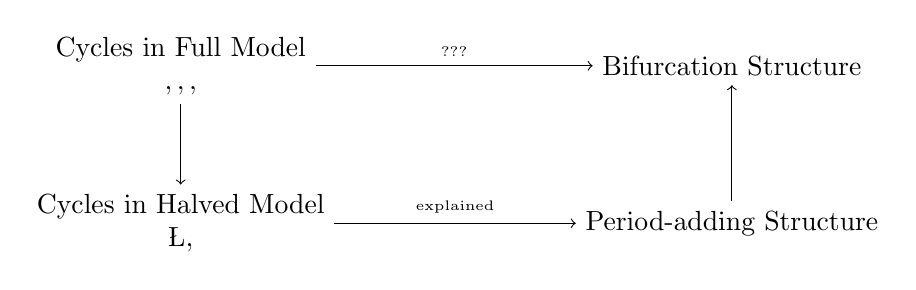
\begin{tikzpicture}[every text node part/.style={align=center}]
			\node (FC) at (0, 2) {Cycles in Full Model \\ $\A, \B, \C, \D$};
			\node (FB) at (7, 2) {Bifurcation Structure};

			\node (HC) at (0, 0) {Cycles in Halved Model \\ $\L, \R$};
			\node (HA) at (7, 0) {Period-adding Structure};

			\draw[->] (FC) -- (HC);
			\draw[->] (HC) -- (HA) node[midway,above] {\tiny explained};
			\draw[->] (HA) -- (FB);
			\draw[->] (FC) -- (FB) node[midway,above] {\tiny ???};
		\end{tikzpicture}
	\end{center}
\end{frame}

\begin{frame}{Some Definitions}
	\vspace{-1em}
	\begin{definition}[Syllables]
		A syllable is a subsequence of maximal length consisting of only one symbol. \\[1em]
		A 2-syllable is a pair of syllables next to each other.
		A 4-syllable is a quadrupel of syllables next to each other.
	\end{definition}
	\pause
	Example: $\L^4\R^3\L^3\R^3$ has the syllables $\L^4$, $\L^3$, and $\R^3$ twice.
	\vspace{1em}
	\begin{itemize}
		\pause
		\item One rotation in the halved model corresponds to one 2-syllable
		\item One rotation in the full model corresponds to one 4-syllable
	\end{itemize}
\end{frame}

\begin{frame}{Translating Symbolic Sequences (1/2)}
	\vspace{-1em}
	\begin{definition}[Translating 4-syllables]
		The function $t$ translates one 4-syllable from the halved model to one 4-syllable in the full model.
		\begin{align*}
			t: \L^a\R^b\L^c\R^d \mapsto \A^a\B^b\C^c\D^d
		\end{align*}
	\end{definition}

	\pause
	From the ad-hoc method:
	\begin{itemize}
		\item We can only translate 4-syllables (two rotations in the halved model) at a time
		\item Especially: We cannot translate a 2-syllable alone
	\end{itemize}
	\pause
	\vspace{1em}
	Number of 2-syllables is odd in the halved model $\Rightarrow$ Wrap around once
\end{frame}

\begin{frame}{Translating Symbolic Sequences (2/2)}
	\begin{itemize}
		\item Start at every 2-syllable of the original symbolic sequence
		\item Omit equivalent resulting symbolic sequences
		      \pause \vspace{2em}
		\item Only the first two 2-syllables matter
		\item Number of 2-syllables is odd $\Rightarrow$ Both results are equivalent
	\end{itemize}
\end{frame}

\begin{frame}{The First Consequences}
	\vspace{3em}
	\begin{theorem}[Periods and Coexistence in the Full Model]
		An $n$-cycle in the halved model manifests as
		\begin{itemize}
			\item a single $2n$-cycle in the full model if it has an odd number of 2-syllables
			\item two coexisting $n$-cycles in the full model if it has an even number of 2-syllables
		\end{itemize}
	\end{theorem}
	%	\pause
	%	Examples:
	%	\begin{itemize}
	%		\item $\L^4\R^3$ (Period 7) manifests as a single cycle $\A^4\B^3\C^4\D^3$ (Period 14)
	%		\item $\L^4\R^3\L^3\R^3$ (Period 13) manifests as two cycles
	%		      \begin{itemize}
	%			      \item $\A^4\B^3\C^3\D^3$ (Period 13) and
	%			      \item $\A^3\B^3\C^4\D^3$ (Period 13)
	%		      \end{itemize}
	%	\end{itemize}
\end{frame}

\begin{frame}{The First Consequences}
	\vspace{2em}
	\begin{theorem}[Coexistence in Child Nodes]
		A node in the Farey-tree is associated
		\begin{itemize}
			\item with a single cycle if
			      \begin{itemize}
				      \item one parent node is associated with 2 coexisting cycles and the other parent node is associated with a single cycle.
			      \end{itemize}
			      \pause
			\item with two coexisting cycles if
			      \begin{itemize}
				      \item both parent nodes are associated with single cycles, or
				      \item both parent nodes are associated with two coexisting cycles each.
			      \end{itemize}
		\end{itemize}
	\end{theorem}
	\pause
	\vspace{1em}
	The third case does not appear in our adding structures (proven in report)
	\begin{tikzpicture}[remember picture,overlay]
		\node[xshift=-11em,yshift=-7.1em] at (current page.north east) {\includegraphics[height=.5 \textheight]{../../Report/Figures/FareyTrees/Minrep_Adding_larger_Full_3/adding.png}};
	\end{tikzpicture}
\end{frame}

\begin{frame}{Explanation of the Period-adding-like Structures}
	\begin{itemize}
		\item Unusual bifurcation structures similar to period-adding structures
		      \pause
		\item Idea: Halved archetypal model
		      \begin{itemize}
			      \item Identified trivial translation from full $\to$ halved
			      \item Identified standard period-adding rules for the structures in the halved model
			      \item Constructed the translation halved $\to$ full
		      \end{itemize}
		      \pause
		\item Explained Period-adding-like structures
		      \begin{itemize}
			      \item Derived rules for periods
			      \item Derived rules for coexistence
			      \item Derived further rules omitted here for brevity
			            %      \begin{itemize}
			            %          \item Combining symbolic sequences
			            %          \item Rotation-tuples
			            %          \item Monotonicity of rotation-tuples
			            %      \end{itemize}
		      \end{itemize}
	\end{itemize}
\end{frame}

%\sectionframe{Conclusion}
\section{Conclusion}

\begin{frame}{Conclusion}
	\begin{itemize}
		\item Confirmed applicability of archetypal map approach
		      \pause
		\item Constructed an archetypal model for the unusual period-incrementing structure
		      \begin{itemize}
			      \item Discovered conditions for the period-incrementing structure
			      \item Investigated border collision bifurcations --- all double
			      \item Found coexistence of up to four cycles
		      \end{itemize}
		      \pause
		\item Period-adding-like structures
		      \begin{itemize}
			      \item Discovered and described an unknown bifurcation structure
			      \item Constructed the halved archetypal model
			      \item Explained the period-adding-like structures with the help of the halved model
		      \end{itemize}
	\end{itemize}
\end{frame}


\thanksframe

%%% Local Variables:
%%% TeX-master: "../Vortrag_Frauenhofer_Weik"
%%% End:
